\chapter{Computational Study: Optical Properties, Thermophysical Fitting,
  and Ablation Threshold Estimation}
\label{ch:computational-study}

\section{Introduction}
\label{sec:ch3-intro}

Chapter~\ref{ch:numerical-methods} established the high-fidelity
numerical solver used throughout the thesis. The present chapter closes
the data-generation side of the retained scope: it documents how
temperature-dependent optical properties, thermophysical constitutive
laws, volumetric source terms, and threshold-search procedures are
assembled into a unified computational pipeline for femtosecond
laser--metal interaction studies. These components provide physically
consistent simulations and threshold labels for the surrogate-modelling
analysis of Chapter~\ref{ch:regression} \cite{Song_2023,Forster_2021,He_2024}.

Sections~\ref{sec:ch3-optical}--\ref{sec:ch3-ablation} proceed in the
same order as the simulation workflow. Section~\ref{sec:ch3-optical}
introduces the temperature-dependent optical models used to evaluate
reflectivity and ballistic-corrected absorption. Section~\ref{sec:ch3-fitting}
then presents the data-driven fitting of the electron heat capacity and
electron--phonon coupling factor. Section~\ref{sec:ch3-heatsource}
connects these constitutive ingredients to the volumetric source model
used in the threshold calculations, and
Section~\ref{sec:ch3-ablation} formulates the certified threshold-search
algorithm together with representative 1D and 2D results. Gold and nickel
serve as the primary illustrative materials, while silver, copper, iron,
and titanium enter the fitting and threshold tables. Unless stated
otherwise, the operating wavelength is fixed at
\(\lambda = \SI{1026}{nm}\).

\section{Temperature-dependent optical models}
\label{sec:ch3-optical}

\subsection{Drude and Lorentz--Drude models}
\label{sec:ch3-optical-drude}

The complex dielectric response is computed from the Lorentz--Drude
formulation introduced in \S\ref{sec:ch1-absorption} through
\eqref{eq:ch1-lorentz-drude}. In this decomposition, the Drude
contribution \(\epsilon_D\) represents the free-electron intraband
response, whereas the Lorentz sum \(\epsilon_L\) captures interband
resonances. The Lorentz--Drude model therefore uses
\(\epsilon = \epsilon_D + \epsilon_L\), while the Drude-only model
retains \(\epsilon = \epsilon_D\) as a reduced approximation
\cite{Tsibidis_2018}.

The temperature dependence enters through the Drude damping rate,
\(\Gamma_0(T_e, T_l)\), introduced in \eqref{eq:ch1-drude-damping}.
We follow the simple Drude model's convention of letting \(\epsilon_\infty \equiv 1\) in the optical model of \eqref{eq:ch1-lorentz-drude}.

Once \(\epsilon = \epsilon_1 + i \epsilon_2\) is obtained, the normal
refractive index and extinction coefficient are computed by \eqref{eq:ch1-coeffs_refractive_index}.

The resulting normal-incidence reflectivity \(R\) and absorption
coefficient \(\alpha\) follow the expressions already defined in
\S\ref{sec:ch1-absorption}; the ballistic-corrected attenuation used in
the heat-source construction is then obtained from
\eqref{eq:ch1-alpha-prime}. Consequently, the optical model feeds the
source term only through the pair
\((R(\lambda, T_e, T_l), \alpha'(\lambda, T_e, T_l))\), without any need
to re-derive the volumetric source itself.

\subsection{Optical properties of gold at \texorpdfstring{\(\SI{1026}{nm}\)}{1026 nm}}
\label{sec:ch3-optical-au}

Table~\ref{tab:ch3-au-optical} summarises the gold parameters inherited
from the Lorentz--Drude model and the room-temperature optical values at
the operating wavelength. The small discrepancy between the full
Lorentz--Drude and Drude-only predictions at \(\SI{1026}{nm}\) indicates
that the interband correction is already weak in the near infrared, even
though it remains visible at shorter wavelengths.

\begin{table}[htbp]
    \centering
    \caption{Optical model parameters and room-temperature properties for Au at \(\lambda = \SI{1026}{nm}\), following \cite{Tsibidis_2018,Lin_2008,Chen_2010}.}
    \label{tab:ch3-au-optical}
    \begin{tabular}{@{}ll@{}}
        \toprule
        \rowcolor{gray!20}
        \textbf{Parameter}                                & \textbf{Value}                             \\
        \midrule
        Plasma frequency                                  & \(\num{1.37e16}\,\si{\radian\per\second}\) \\
        Number of Lorentz oscillators                     & 6                                          \\
        Oscillator strengths                              & \(0.76, 0.024, 0.01, 0.071, 0.601, 4.384\) \\
        Damping coefficients                              & \(0.053, 0.241, 0.345\)\,eV                \\
        Resonance frequencies                             & \(0.000, 0.415, 0.830\)\,eV                \\
        \(R_{\mathrm{LD}}\)                               & 0.966                                      \\
        \(R_{\mathrm{D}}\)                                & 0.980                                      \\
        \(\Delta R\)                                      & \(-0.014\)                                 \\
        \(\alpha_{\mathrm{LD}}\)                          & \(\SI{75.550}{\per\micro\metre}\)          \\
        \(\alpha_{\mathrm{D}}\)                           & \(\SI{78.717}{\per\micro\metre}\)          \\
        \(\Delta \alpha\)                                 & \(-\SI{3.166}{\per\micro\metre}\)          \\
        \(\delta_{\mathrm{LD}} = 1/\alpha_{\mathrm{LD}}\) & \(\SI{13.236}{nm}\)                        \\
        \(\delta_{\mathrm{D}} = 1/\alpha_{\mathrm{D}}\)   & \(\SI{12.704}{nm}\)                        \\
        \bottomrule
    \end{tabular}
\end{table}

Figure~\ref{fig:ch3-au-heatmap} shows the gold reflectivity and
absorption landscape under the Drude approximation. Over the
temperature range relevant to the ablation calculations, the variation of
\(\alpha\) is more pronounced than that of \(R\), which is consistent
with the damping increase encoded by \eqref{eq:ch1-drude-damping}.

\begin{figure}[htbp]
    \centering
    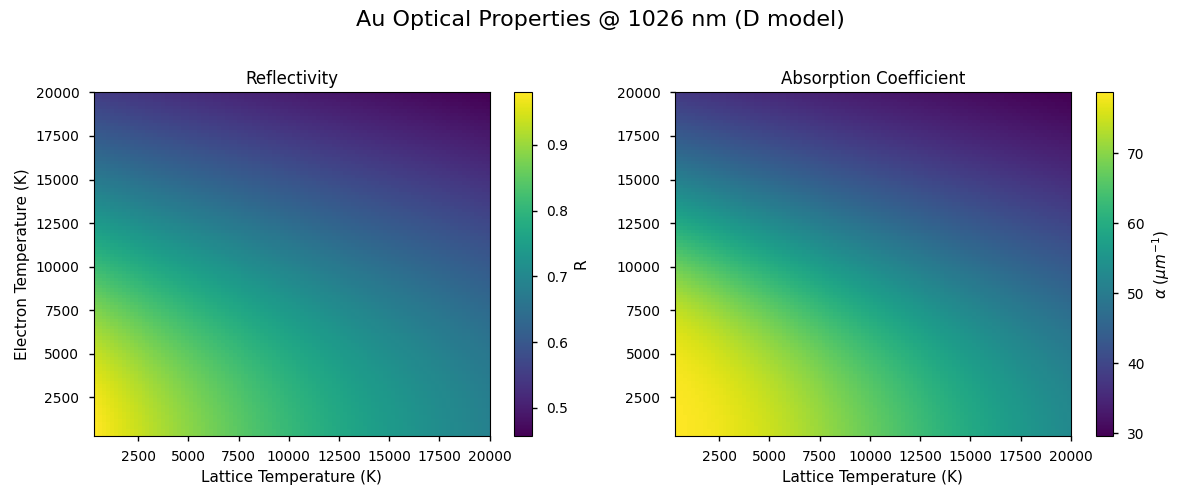
\includegraphics[width=0.82\linewidth]{figures/ch3/heatmaps_1026nm_D.png}
    \caption{Heatmap of reflectivity \(R\) and absorption coefficient \(\alpha\) as functions of \(T_e\) and \(T_l\) for Au at \(\lambda = \SI{1026}{nm}\), Drude model. The strong \(T_e\) dependence of \(\alpha\) reflects the increasing electron-phonon scattering at elevated electron temperatures.}
    \label{fig:ch3-au-heatmap}
\end{figure}

The spectral comparison in Fig.~\ref{fig:ch3-au-spectrum} confirms that
the Lorentz contribution is primarily relevant below the visible and
near-visible regime, while the near-infrared operating window is already
well described by the Drude response alone.

\begin{figure}[htbp]
    \centering
    \subfloat[Au spectrum from \(\SI{10}{nm}\) to \(\SI{1200}{nm}\).\label{fig:ch3-au-spectrum-wide}]{%
        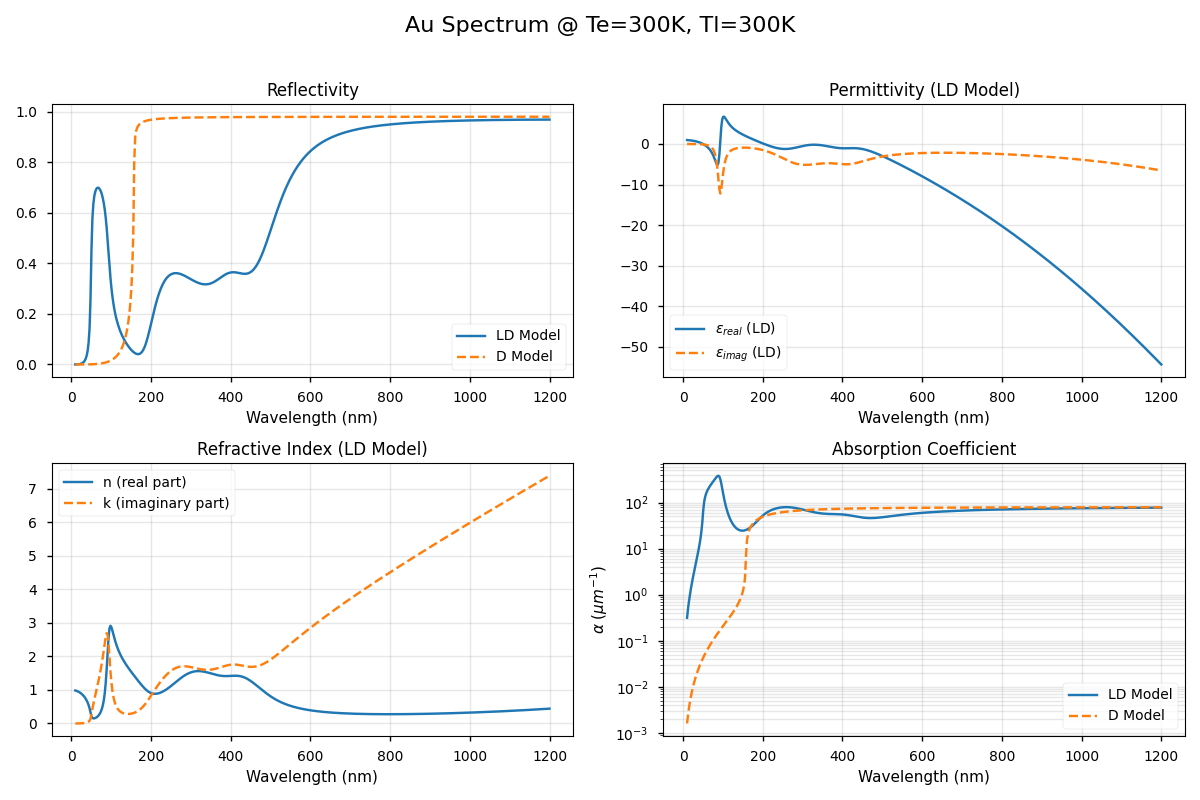
\includegraphics[width=0.48\linewidth]{figures/ch3/spectrum_comparison_10_1200_RT.png}
    }\hfill
    \subfloat[Au spectrum in the \(\SI{800}{nm}\)--\(\SI{1200}{nm}\) operating window.\label{fig:ch3-au-spectrum-nearir}]{%
        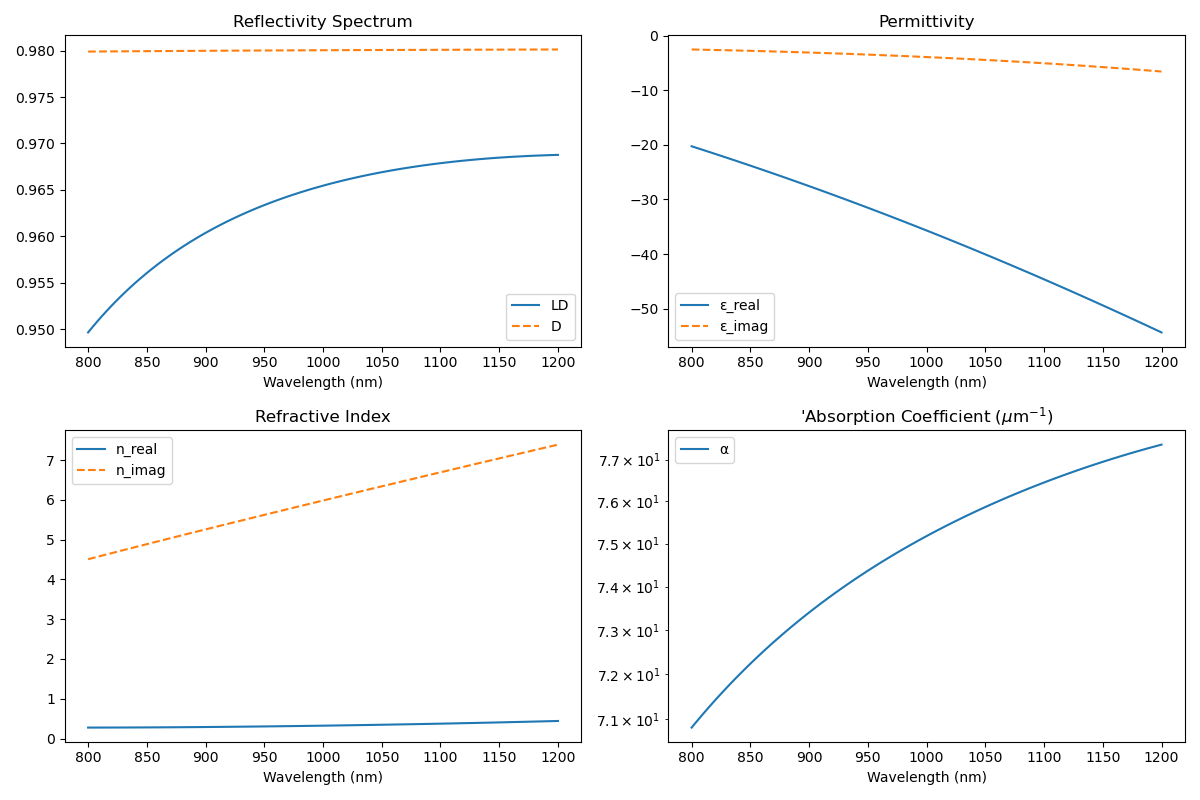
\includegraphics[width=0.48\linewidth]{figures/ch3/spectrum_comparison_RT.png}
    }
    \caption{Optical spectrum comparison for Au at room temperature: (a) \(\SI{10}{nm}\)--\(\SI{1200}{nm}\), (b) \(\SI{800}{nm}\)--\(\SI{1200}{nm}\) operating range. The LD and D models agree closely beyond \(\SI{600}{nm}\); the interband contribution (Lorentz terms) is significant below that threshold. Compare with \cite{Ren_2011}, Figs.~1--2.}
    \label{fig:ch3-au-spectrum}
\end{figure}

The equal-temperature series in Fig.~\ref{fig:ch3-au-tempseries}
illustrates the gradual decrease of reflectivity and the corresponding
increase of attenuation as the metal is heated from ambient conditions.

\begin{figure}[htbp]
    \centering
    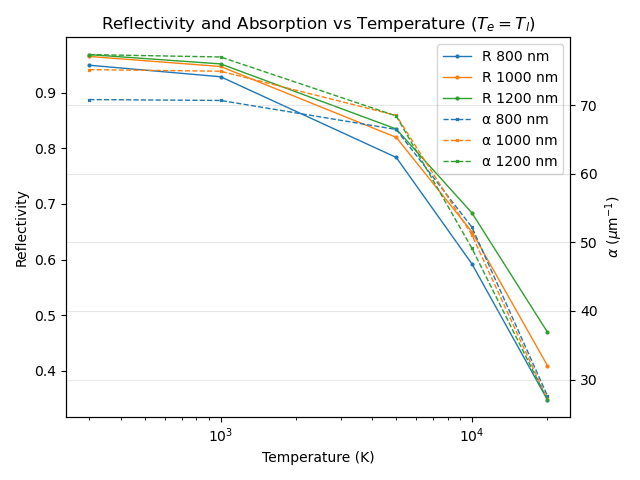
\includegraphics[width=0.62\linewidth]{figures/ch3/tempseries_multi_LD.png}
    \caption{Temperature series of \(R\) and \(\alpha\) for Au at \(\lambda = \SI{1026}{nm}\), Lorentz--Drude model (\(T_e = T_l\)).}
    \label{fig:ch3-au-tempseries}
\end{figure}

\subsection{Optical properties of nickel at \texorpdfstring{\(\SI{1026}{nm}\)}{1026 nm}}
\label{sec:ch3-optical-ni}

Nickel exhibits a substantially stronger discrepancy between the two
optical models than gold. In particular, the room-temperature
reflectivity difference reaches \(\Delta R = -0.246\), which implies a
marked change in the absorbed fraction of the incident pulse. This is a
direct consequence of the five Lorentz oscillators required to represent
the interband structure of nickel near the operating wavelength.

\begin{table}[htbp]
    \centering
    \caption{Optical model parameters and room-temperature properties for Ni at \(\lambda = \SI{1026}{nm}\), following \cite{Tsibidis_2018,Lin_2008,Chen_2010}.}
    \label{tab:ch3-ni-optical}
    \begin{tabular}{@{}ll@{}}
        \toprule
        \rowcolor{gray!20}
        \textbf{Parameter}                                & \textbf{Value}                             \\
        \midrule
        Plasma frequency                                  & \(\num{2.42e16}\,\si{\radian\per\second}\) \\
        Number of Lorentz oscillators                     & 5                                          \\
        Oscillator strengths                              & \(0.096, 0.100, 0.135, 0.106, 0.729\)      \\
        Damping coefficients                              & \(0.048, 4.511, 1.334\)\,eV                \\
        Resonance frequencies                             & \(0.000, 0.174, 0.582\)\,eV                \\
        \(R_{\mathrm{LD}}\)                               & 0.722                                      \\
        \(R_{\mathrm{D}}\)                                & 0.969                                      \\
        \(\Delta R\)                                      & \(-0.246\)                                 \\
        \(\alpha_{\mathrm{LD}}\)                          & \(\SI{62.876}{\per\micro\metre}\)          \\
        \(\alpha_{\mathrm{D}}\)                           & \(\SI{48.397}{\per\micro\metre}\)          \\
        \(\Delta \alpha\)                                 & \(\SI{14.479}{\per\micro\metre}\)          \\
        \(\delta_{\mathrm{LD}} = 1/\alpha_{\mathrm{LD}}\) & \(\SI{15.904}{nm}\)                        \\
        \(\delta_{\mathrm{D}} = 1/\alpha_{\mathrm{D}}\)   & \(\SI{20.663}{nm}\)                        \\
        \bottomrule
    \end{tabular}
\end{table}

\begin{figure}[htbp]
    \centering
    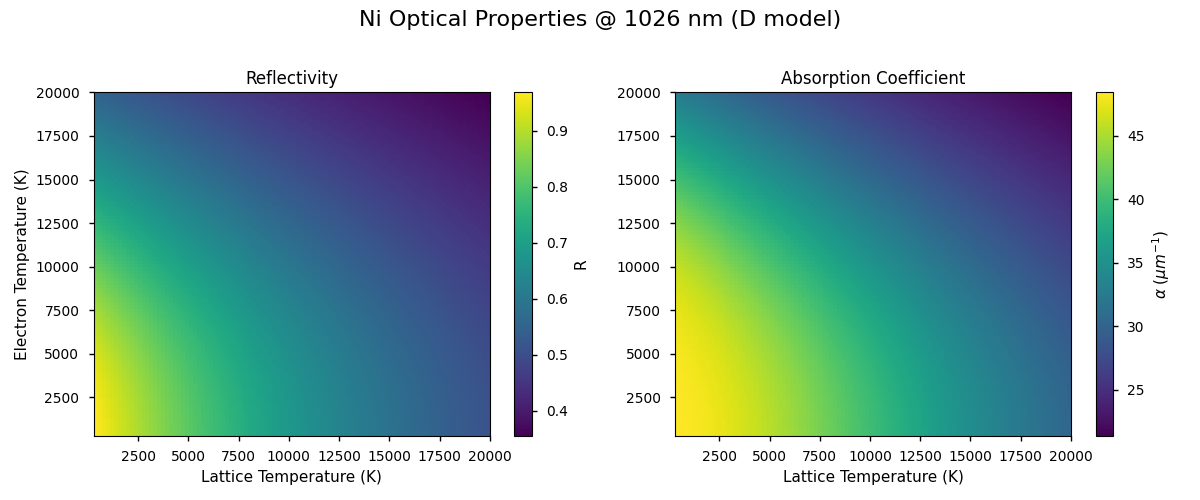
\includegraphics[width=0.82\linewidth]{figures/ch3/Ni_heatmap_1026nm_D.png}
    \caption{Heatmap of reflectivity \(R\) and absorption coefficient \(\alpha\) as functions of \(T_e\) and \(T_l\) for Ni at \(\lambda = \SI{1026}{nm}\), Drude model.}
    \label{fig:ch3-ni-heatmap}
\end{figure}

\begin{figure}[htbp]
    \centering
    \subfloat[Ni spectrum from \(\SI{10}{nm}\) to \(\SI{1200}{nm}\).\label{fig:ch3-ni-spectrum-wide}]{%
        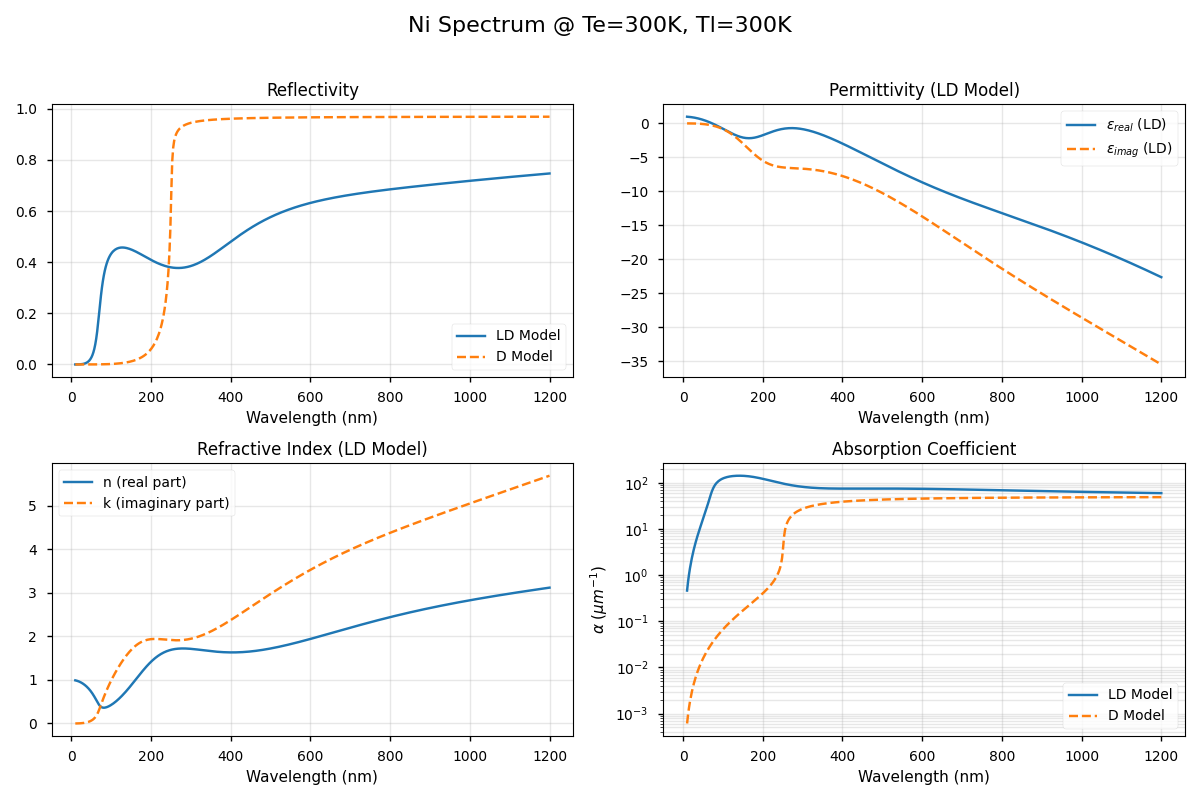
\includegraphics[width=0.48\linewidth]{figures/ch3/Ni_spectrum_comparison_10_1200_RT.png}
    }\hfill
    \subfloat[Ni spectrum in the \(\SI{800}{nm}\)--\(\SI{1200}{nm}\) operating window.\label{fig:ch3-ni-spectrum-nearir}]{%
        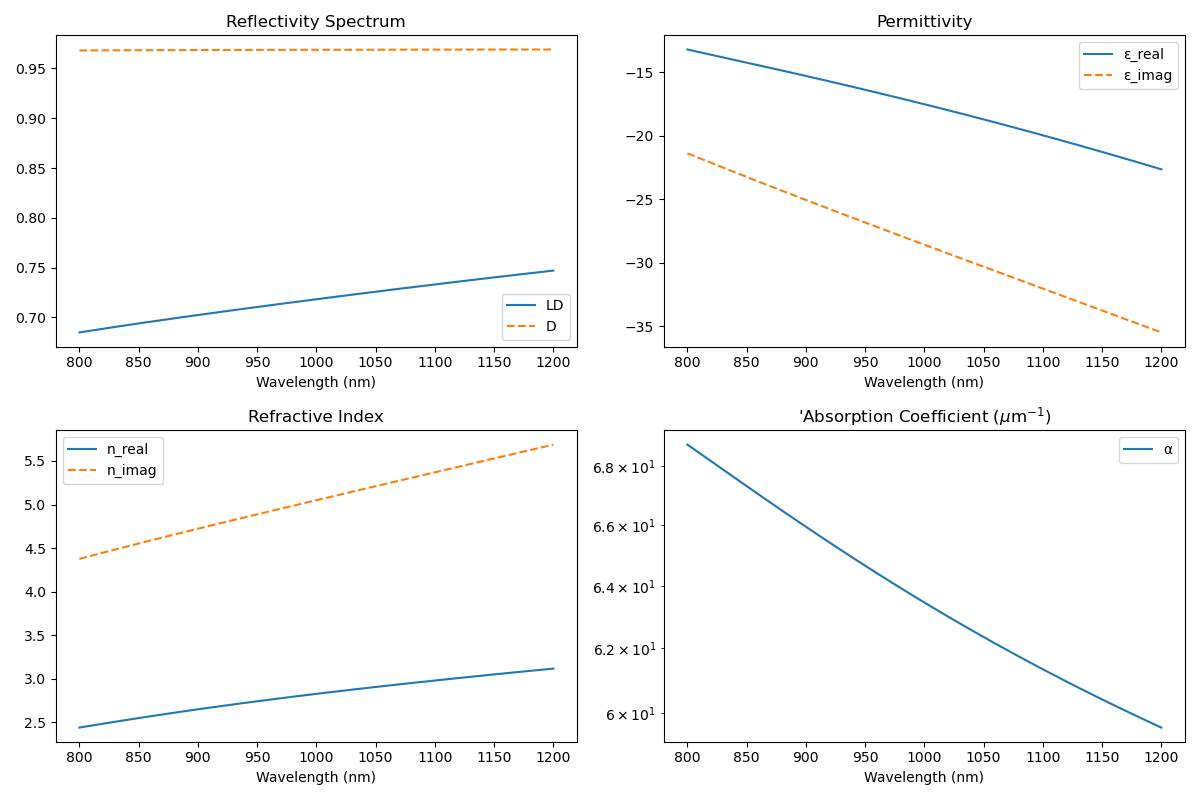
\includegraphics[width=0.48\linewidth]{figures/ch3/Ni_spectrum_comparison_RT.png}
    }
    \caption{Optical spectrum comparison for Ni at room temperature: (a) \(\SI{10}{nm}\)--\(\SI{1200}{nm}\), (b) \(\SI{800}{nm}\)--\(\SI{1200}{nm}\) operating range. The Lorentz contribution remains significant at \(\SI{1026}{nm}\), so the Drude-only model substantially overestimates reflectivity and underestimates absorption.}
    \label{fig:ch3-ni-spectrum}
\end{figure}

\begin{figure}[htbp]
    \centering
    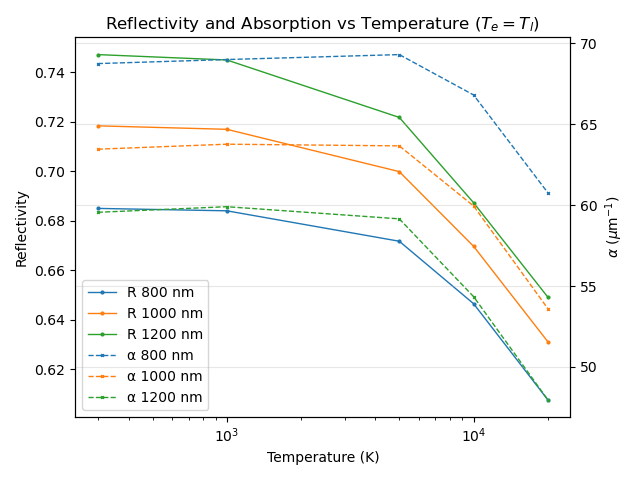
\includegraphics[width=0.62\linewidth]{figures/ch3/Ni_tempseries_multi_LD.png}
    \caption{Temperature series of \(R\) and \(\alpha\) for Ni at \(\lambda = \SI{1026}{nm}\), Lorentz--Drude model (\(T_e = T_l\)).}
    \label{fig:ch3-ni-tempseries}
\end{figure}

For nickel, the five Lorentz oscillators encode interband transitions that
remain active near \(\SI{1026}{nm}\). The resulting discrepancy between the
Lorentz--Drude and Drude-only models propagates directly into the
absorbed-intensity term \((1-R)\), and therefore into the volumetric heat
source used by the pTTM solver.

\subsection{Debye model for water}
\label{sec:ch3-optical-water}

For completeness, the dielectric response of water is modelled by the
two-pole Debye bipolar expression
\begin{equation}
    \epsilon_{DB}(\omega)
    \coloneqq
    1
    +
    \sum_{j=1}^{2}
    a_j
    \bigl(1 - i \tau_j \omega\bigr)^{-(1-\nu_j)}
    \bigl(1 - i \tau_f \omega\bigr)^{-1},
    \label{eq:ch3-debye}
\end{equation}
where \(a_j\) are pole amplitudes, \(\tau_j\) are relaxation times,
\(\tau_f\) is the fast relaxation scale, and \(\nu_j\) are the
Cole--Cole exponents \cite{Rusiniak_2000}.
This model is retained for completeness in the
source-generation pipeline, but water is not a primary material in the
ablation-threshold study reported below.

\section{Electron heat capacity and electron--phonon coupling: data-driven fitting}
\label{sec:ch3-fitting}

The optical model determines how laser energy enters the material, but
the subsequent thermal evolution depends equally on the constitutive
closures for \(C_e(T_e)\) and \(G(T_e)\).
These functions are fitted from ab-initio data and then supplied to the nonlinear solver introduced in
Chapter~\ref{ch:numerical-methods}.

\subsection{Data acquisition and preprocessing}
\label{sec:ch3-fitting-data}

The raw thermophysical data are taken from density-of-states calculations
performed with VASP and reported by Fang et al.~\cite{Fang_2012}. For
each material, the input arrays provide \(C_e(T_e)\) and \(G(T_e)\) on a
temperature grid of 1000 points extending to approximately
\(\SI{1e5}{K}\), with temperatures stored in units of \(10^4\,\si{K}\) and
property values stored in scaled SI form.

The raw variables are converted to physical units through the mappings
\[
    T_{\mathrm{raw}}
    \mapsto
    T = 10^4 T_{\mathrm{raw}}\,\si{K},
    \qquad
    C_{e,\mathrm{raw}}
    \mapsto
    C_e = 10^5 C_{e,\mathrm{raw}},
    \qquad
    G_{\mathrm{raw}}
    \mapsto
    G = 10^{17} G_{\mathrm{raw}}.
\]
After this rescaling, the arrays may be interpreted directly in the SI
units required by the pTTM closures.

\subsection{Piecewise polynomial fitting}
\label{sec:ch3-fitting-poly}

The ab-initio curves exhibit clear changes of curvature, particularly at
moderate and high electron temperatures. To capture this behaviour, the
temperature domain is split at a material-dependent threshold
\(T_{\mathrm{th}}\), and piecewise polynomial fits are used:
\begin{equation}
    f_{\mathrm{pw}}(T_e)
    =
    \begin{cases}
        p_{\mathrm{low}}(T_e),  & T_e \leq T_{\mathrm{th}}, \\
        p_{\mathrm{high}}(T_e), & T_e > T_{\mathrm{th}},
    \end{cases}
    \label{eq:ch3-piecewise-poly}
\end{equation}
where \(p_{\mathrm{low}}\) and \(p_{\mathrm{high}}\) are least-squares
polynomials of degrees \(n_{\mathrm{low}}\) and \(n_{\mathrm{high}}\),
respectively.

The material-specific thresholds and polynomial orders used throughout
the simulations are listed in Table~\ref{tab:ch3-fitting-params}. Iron
requires a degree-12 polynomial on the high-temperature side in order to
resolve its stronger curvature, while nickel and titanium enforce
quadratic low-temperature fits for \(G\).

\begin{table}[htbp]
    \centering
    \caption{Threshold temperatures and polynomial orders used in the piecewise fits of \(C_e(T_e)\) and \(G(T_e)\).}
    \label{tab:ch3-fitting-params}
    \begin{tabular}{@{}lccc@{}}
        \toprule
        \rowcolor{gray!20}
        \textbf{Material} & \(\boldsymbol{T_{\mathrm{th}}}\) \textbf{(K)} & \(\boldsymbol{C_e}\) \textbf{degrees} & \(\boldsymbol{G}\) \textbf{degrees} \\
        \midrule
        Au                & 2500                                          & \((1, 11)\)                           & \((0, 15)\)                         \\
        Ag                & 4250                                          & \((1, 11)\)                           & \((0, 15)\)                         \\
        Cu                & 2250                                          & \((1, 11)\)                           & \((0, 15)\)                         \\
        Fe                & 750                                           & \((1, 12)\)                           & \((0, 15)\)                         \\
        Ni                & 500                                           & \((1, 12)\)                           & \((2, 15)\)                         \\
        Ti                & 1000                                          & \((1, 11)\)                           & \((2, 15)\)                         \\
        \bottomrule
    \end{tabular}
\end{table}

\subsection{Constant and variable approximations}
\label{sec:ch3-fitting-approx}

For the linear solver of Chapter~\ref{ch:numerical-methods}, the
constitutive law is frozen at room temperature and written in the form
\[
    C_e \approx \gamma T_{\mathrm{RT}},
    \qquad
    G \approx G_0,
\]
where \(\gamma\) is the Sommerfeld coefficient and \(G_0\) is the
room-temperature electron--phonon coupling. These constants reproduce the
Au parameter set already reported in \eqref{eq:ch2-linear-params}.

For the nonlinear solver, the fitted piecewise functions
\eqref{eq:ch3-piecewise-poly} are inserted directly into the
dimensionless constitutive coefficients
\eqref{eq:ch2-dimensionless-coeffs} through
\(C_e(T_{\mathrm{ref}}u)\) and \(G(T_{\mathrm{ref}}u)\). The same fit is
therefore used consistently in both the physical-unit post-processing of
this chapter and the dimensionless solver formulation of Chapter~2.

An alternative closed-form expression is available through
\eqref{eq:ch1-G_closed_formula}, which follows from a constant
density-of-states approximation together with linear-response
electron--phonon coupling. That approximation is useful as a compact
baseline, but it does not capture the pronounced nonlinear features
visible in the ab-initio curves, especially for nickel and titanium.

\subsection{Fitting results and validation}
\label{sec:ch3-fitting-results}

Table~\ref{tab:ch3-fitting-errors} compares the fitted low-temperature
coefficients against the Chen et al.~\cite{Chen_2010} reference values.
Two distinct discrepancy measures must be distinguished. The relative
errors associated with the \(\gamma\) column are
\(+1.5\%\) for Au, \(-0.8\%\) for Ag, \(+10.1\%\) for Cu, and
\(-59.8\%\) for Ni. By contrast, the \(G_0\) comparison yields
\(+24.8\%\) for Au, \(-21.6\%\) for Ag, and \(-44.6\%\) for Cu. Nickel
does not admit a meaningful \(G_0\) comparison in the same linearised
form, because the fitted low-temperature behaviour is already quadratic
rather than linear. This observation explains the large discrepancy with
the linear approximation implicit in \cite{Chen_2010}.

\begin{table}[htbp]
    \centering
    \caption{Comparison between low-temperature thermophysical fits and the room-temperature approximations reported by \cite{Chen_2010}.}
    \label{tab:ch3-fitting-errors}
    \begin{tabular}{@{}lcccccc@{}}
        \toprule
        \rowcolor{gray!20}
        \textbf{Metal} & \(\boldsymbol{\gamma_{\mathrm{fit}}}\) & \(\boldsymbol{\gamma_{\mathrm{ref}}}\) & \textbf{Error (\%)} & \(\boldsymbol{G_{0,\mathrm{fit}}}\)                                               & \(\boldsymbol{G_{0,\mathrm{ref}}}\) & \textbf{Error (\%)} \\
        \midrule
        Au             & 69.05                                  & 68                                     & \(+1.5\)            & 2.62                                                                              & 2.10                                & \(+24.8\)           \\
        Ag             & 62.52                                  & 63                                     & \(-0.8\)            & 2.43                                                                              & 3.10                                & \(-21.6\)           \\
        Cu             & 106.76                                 & 97                                     & \(+10.1\)           & 5.54                                                                              & 10.0                                & \(-44.6\)           \\
        Ni             & 427.84                                 & 1065                                   & \(-59.8\)           & \multicolumn{3}{c}{Quadratic low-\(T_e\) behaviour; no direct \(G_0\) comparison}                                                             \\
        \bottomrule
    \end{tabular}
\end{table}

Figures~\ref{fig:ch3-au-ce-g} and~\ref{fig:ch3-ni-ce-g} show the fitted
curves for gold and nickel across the full temperature range and over the
simulation-relevant window \([\SI{100}{K}, \SI{5000}{K}]\). The latter
window is the most relevant one for threshold estimation, because it
contains the regime in which lattice heating becomes dominant while still
retaining the leading nonlinear corrections to the electron subsystem.

\begin{figure}[H]
    \centering
    \subfloat[Full temperature range.\label{fig:ch3-au-ce-g-full}]{%
        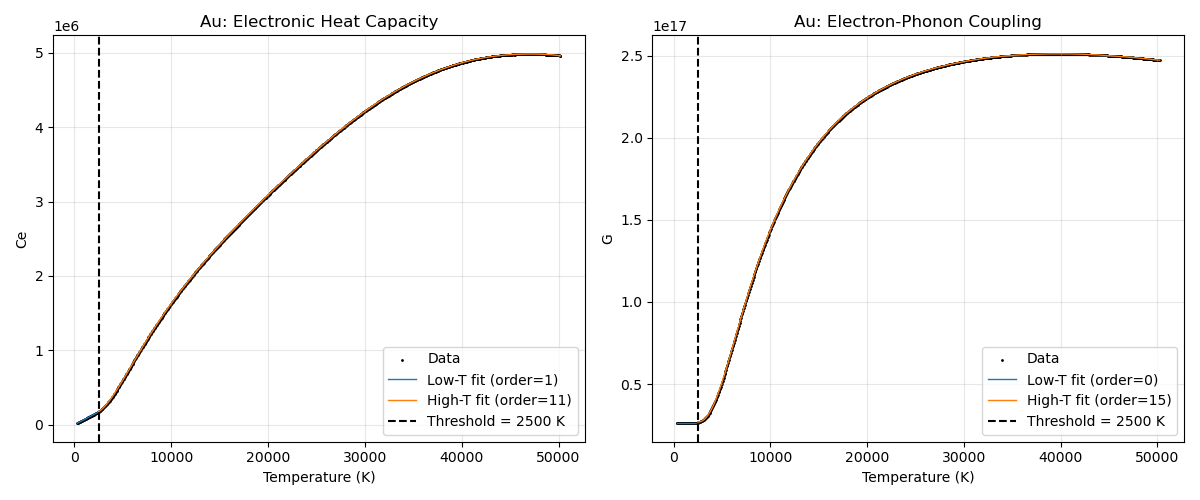
\includegraphics[width=0.48\linewidth]{figures/ch3/Au_Ce_G_curves.png}
    }\hfill
    \subfloat[Focused range from \SI{100}{K} to \SI{5000}{K}.\label{fig:ch3-au-ce-g-focus}]{%
        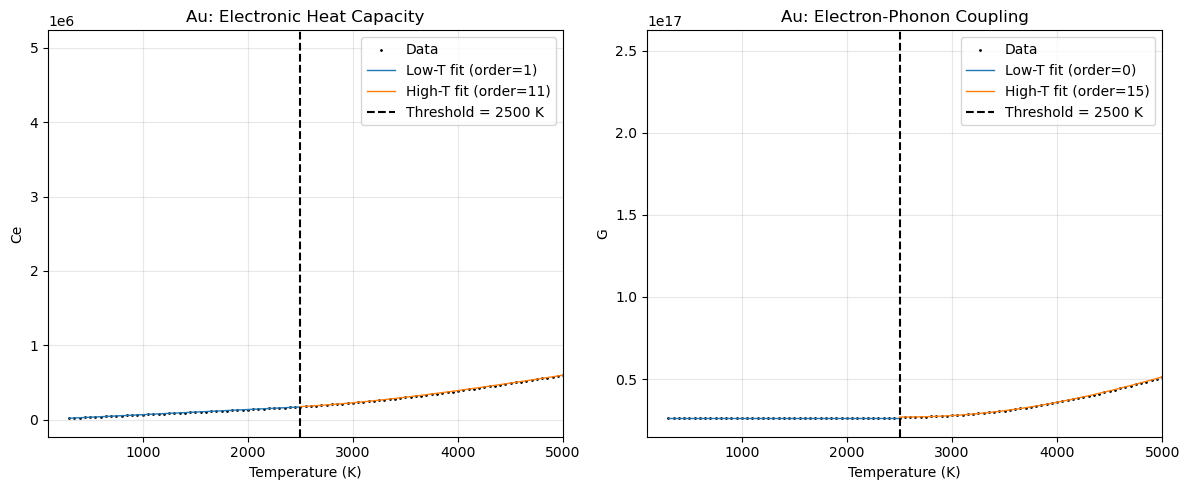
\includegraphics[width=0.48\linewidth]{figures/ch3/Au_Ce_G_curves_focused.png}
    }
    \caption{Piecewise polynomial fits of \(C_e(T_e)\) and \(G(T_e)\) for gold, based on VASP density-of-states data \cite{Fang_2012}. The left panel shows the full temperature range, while the right panel focuses on the interval most relevant to the ablation simulations.}
    \label{fig:ch3-au-ce-g}
\end{figure}

\begin{figure}[H]
    \centering
    \subfloat[Full temperature range.\label{fig:ch3-ni-ce-g-full}]{%
        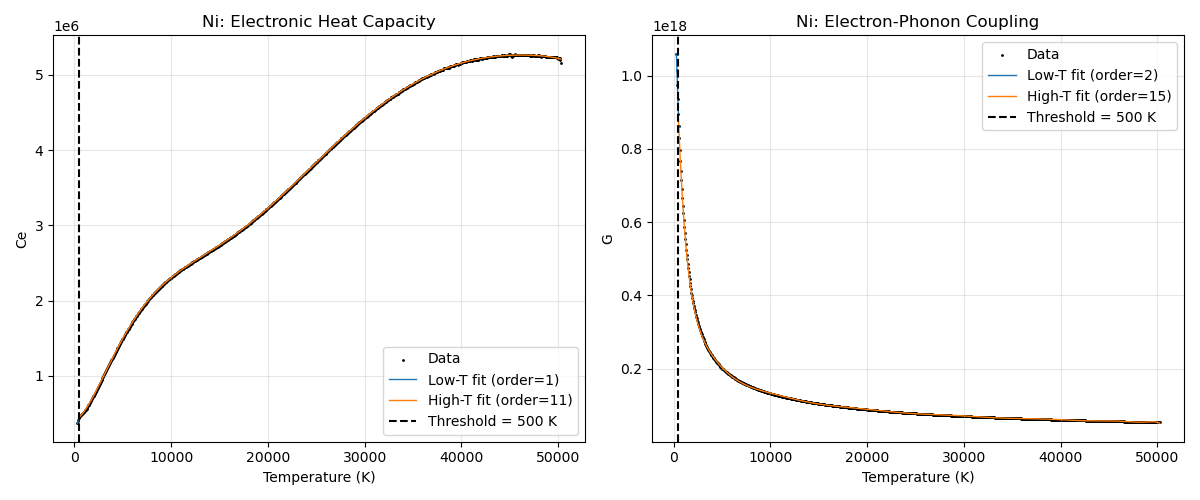
\includegraphics[width=0.48\linewidth]{figures/ch3/Ni_Ce_G_curves.png}
    }\hfill
    \subfloat[Focused range from \SI{100}{K} to \SI{5000}{K}.\label{fig:ch3-ni-ce-g-focus}]{%
        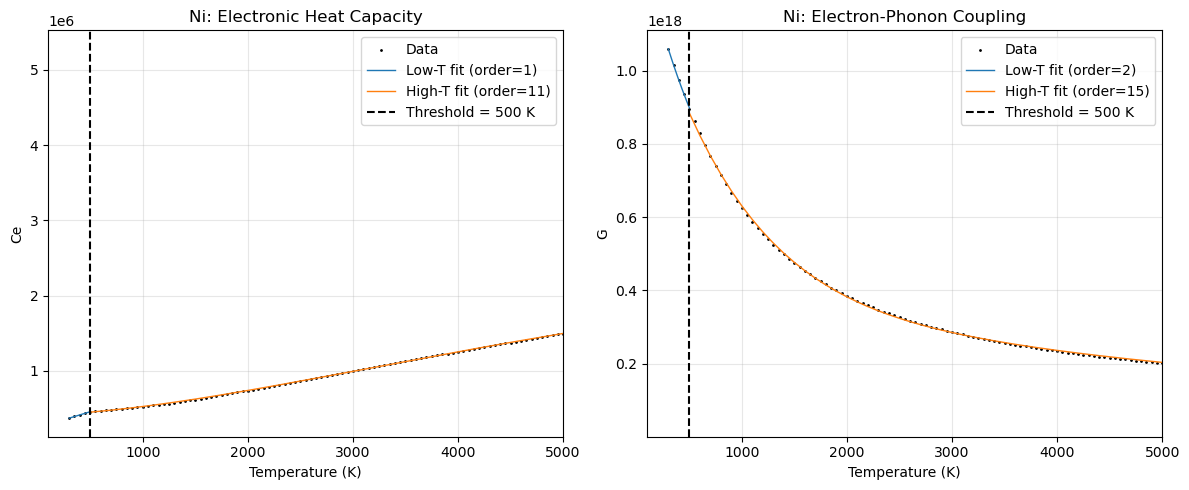
\includegraphics[width=0.48\linewidth]{figures/ch3/Ni_Ce_G_curves_focused.png}
    }
    \caption{Piecewise polynomial fits of \(C_e(T_e)\) and \(G(T_e)\) for nickel, based on VASP density-of-states data \cite{Fang_2012}.}
    \label{fig:ch3-ni-ce-g}
\end{figure}

For direct comparison with the ab-initio gold benchmark reported by Fang
et al., see Fig.~\ref{fig:ch1-ce-g-literature} in Chapter~1, where the
original literature curves are presented.

\section{Volumetric source model for threshold calculations}
\label{sec:ch3-heatsource}

The threshold calculations use the single-beam volumetric source
\eqref{eq:ch1-ulp_heat_source}, with the optical response
\((R, \alpha')\) computed from the temperature-dependent models of
\S\ref{sec:ch3-optical}. At the numerical level, the source
decomposition of \eqref{eq:ch2-source-decomp} is especially convenient:
the temperature-independent Gaussian intensity profile is separated from
the temperature-dependent attenuation factor
\(K_{\mathrm{src}}\), which carries the ballistic correction and the
finite-thickness factor. The one- and two-dimensional reductions then
follow directly from the source-model reductions detailed in
\S\ref{sec:ch1-heat-source}.

In the retained threshold study, the source is the unpatterned
single-beam source. The relevant source parameters are therefore the
operating wavelength, pulse duration, beam radius in the two-dimensional
runs, incident fluence, and the temperature-dependent optical quantities
entering \((1-R)\alpha'\). Their numerical values are reported with the
threshold-study configurations in Tables~\ref{tab:ch3-1d-params}
and~\ref{tab:ch3-2d-params}.

\section{Damage threshold estimation}
\label{sec:ch3-ablation}

\subsection{Damage criterion and threshold definition}
\label{sec:ch3-ablation-criterion}

For each material and pulse configuration, define the peak lattice
temperature as a function of the incident fluence,
\[
    T_{l,\max}(F)
    \coloneqq
    \max_{(t, \mathbf{r}) \in [0, \tau_f] \times \Omega}
    T_l(\mathbf{r}, t; F).
\]
The present study adopts the melting-onset criterion
\(T_{l,\max}(F) \geq T_m\), where \(T_m\) is the equilibrium melting
temperature of the target material. The corresponding threshold fluence is
\begin{equation}
    F_{\mathrm{th}}
    \coloneqq
    \inf\{F > 0 : T_{l,\max}(F) \geq T_m\}.
    \label{eq:ch3-threshold}
\end{equation}
The search strategy assumes that \(T_{l,\max}(F)\) is non-decreasing in
\(F\) for fixed material and pulse parameters.

This melting-based definition is standard in thermal pTTM studies, while
the surrounding ablation literature also includes hydrodynamic, phase
explosion, and material-removal criteria depending on the modelling scope
\cite{Hashida_2001,Gamaly_2002,Forster_2021,Cheng_2016,Zhou_2022,Wang_2024}.
In the present computational setting, the melting threshold provides a
well-defined and reproducible label that can be extracted consistently
from both the linear and nonlinear solver outputs.

The threshold detector operates on a finite observation window centred at
\(t_{\mathrm{centre}} = 3\tau_p\) with half-width \(w_h \tau_p\), clipped to the
simulation interval \([0, \tau_f]\). This choice concentrates
the search on the temporal neighbourhood in which the lattice response is
expected to attain its maximum under single-pulse excitation.

All experiments of this subsection were conducted using a single NVIDIA RTX 3090 Ti GPU.

\subsection{Exponential bracketing and bisection refinement}
\label{sec:ch3-ablation-algorithm}

The complete derivation of the search algorithm, including the
equilibration analysis, cost bounds, and uncertainty propagation, is
deferred to Appendix~\ref{app:equilibration-ablation}. In the main text it
is sufficient to record the two central estimates. If the exponential
phase starts from \(F_{\mathrm{init}}\) and grows by factor \(r > 1\),
then the number of exponential evaluations satisfies
\begin{equation}
    n_{\exp}
    \leq
    \left\lceil
    \frac{\log(F_{\mathrm{th}} / F_{\mathrm{init}})}{\log r}
    \right\rceil,
    \label{eq:ch3-exp-cost}
\end{equation}
while the subsequent bisection stage requires
\begin{equation}
    k
    \geq
    \left\lceil
    \log_2\!\left(
    \frac{F_u^{(0)} - F_l^{(0)}}{\varepsilon}
    \right)
    \right\rceil
    \label{eq:ch3-bis-cost}
\end{equation}
iterations to reduce the bracket width below the tolerance
\(\varepsilon\). The final midpoint estimate \(\hat{F}_{\mathrm{th}}\)
therefore satisfies the rigorous uncertainty bound
\(|\hat{F}_{\mathrm{th}} - F_{\mathrm{th}}| \leq \delta F_{\mathrm{bis}}
\coloneqq (F_u - F_l)/2\) \cite{Beigel_1990}.

\begin{figure}[htbp]
    \centering
    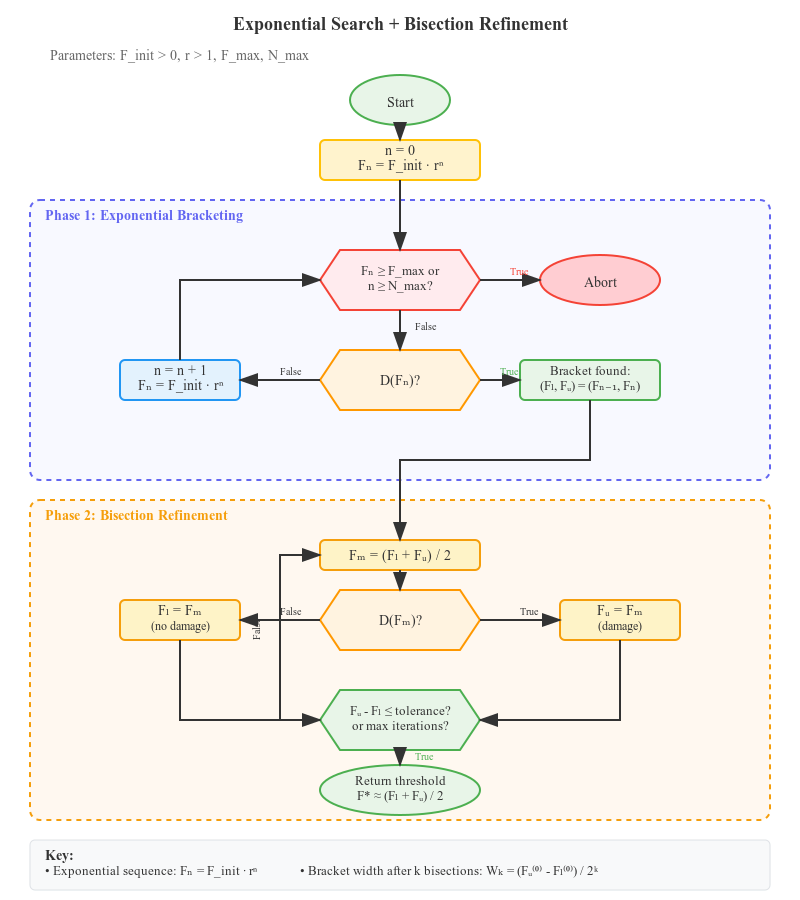
\includegraphics[width=0.92\linewidth]{figures/ch3/exponential_bisection_flowchart.png}
    \caption{Flowchart of the exponential-search + bisection-refinement algorithm for ablation threshold detection. The exponential phase rapidly brackets \(F_{\mathrm{th}}\) using multiplicative factor \(r = 2\); the bisection phase refines the bracket to tolerance \(\varepsilon = \SI{0.5}{\joule\per\square\metre}\).}
    \label{fig:ch3-flowchart}
\end{figure}

\begin{table}[htbp]
    \centering
    \caption{Algorithm parameters used in the exponential-search + bisection threshold detector.}
    \label{tab:ch3-alg-params}
    \begin{tabular}{@{}lll@{}}
        \toprule
        \rowcolor{gray!20}
        \textbf{Parameter}            & \textbf{Value}                        & \textbf{Description}                                     \\
        \midrule
        \texttt{exp\_factor}          & 2.0                                   & Multiplicative growth factor per step                    \\
        \texttt{exp\_max}             & \(\num{1e6}\)                         & Maximum allowed fluence \(\si{\joule\per\square\metre}\) \\
        \texttt{exp\_max\_steps}      & 30                                    & Maximum exponential-search iterations                    \\
        \texttt{bisection\_tol}       & \(\SI{0.5}{\joule\per\square\metre}\) & Bisection stopping tolerance                             \\
        \texttt{bisection\_max\_iter} & 20                                    & Maximum bisection iterations                             \\
        \texttt{window\_half\_mult}   & 2.0                                   & Half-width multiplier for the analysis window            \\
        \bottomrule
    \end{tabular}
\end{table}

\subsection{Simulation parameters}
\label{sec:ch3-ablation-simparams}

The threshold study uses a common physical configuration across the linear
and nonlinear solvers, with both variants run at a representative
resolution in one and two spatial dimensions. The resulting parameter sets
are listed in Tables~\ref{tab:ch3-1d-params} and~\ref{tab:ch3-2d-params}.
All simulations correspond to a single Gaussian pulse in the ULP regime,
and all reported threshold values are expressed in physical units.

\begin{table}[htbp]
    \centering
    \caption{1D threshold-study parameters.}
    \label{tab:ch3-1d-params}
    \begin{tabular}{@{}lc@{}}
        \toprule
        \rowcolor{gray!20}
        \textbf{Parameter}        & \textbf{Linear \& Nonlinear} \\
        \midrule
        Film thickness \(z_t\)    & \(\SI{1}{\micro\metre}\)     \\
        Evolution time \(\tau_f\) & \(\SI{100}{\pico\second}\)   \\
        Temporal points \(N_t\)   & 1001                         \\
        Depth points \(N_z\)      & 201                          \\
        Pulse duration \(\tau_p\) & \(\SI{10}{\pico\second}\)    \\
        wavelength \(\lambda_L\)  & \(\SI{1030}{\nano\metre}\)   \\
        \bottomrule
    \end{tabular}
\end{table}

\begin{table}[htbp]
    \centering
    \caption{2D threshold-study parameters.}
    \label{tab:ch3-2d-params}
    \begin{tabular}{@{}ll@{}}
        \toprule
        \rowcolor{gray!20}
        \textbf{Parameter}         & \textbf{Linear \& Nonlinear} \\
        \midrule
        Film width \(x_w\)         & \(\SI{1}{\micro\metre}\)     \\
        Film thickness \(z_t\)     & \(\SI{1}{\micro\metre}\)     \\
        Evolution time \(\tau_f\)  & \(\SI{100}{\pico\second}\)   \\
        Temporal points \(N_t\)    & 501                          \\
        \(x\)-points \(N_x\)       & 101                          \\
        \(z\)-points \(N_z\)       & 101                          \\
        Pulse duration \(\tau_p\)  & \(\SI{10}{\pico\second}\)    \\
        Beam-radius factor \(R_0\) & 4.0                          \\
        wavelength \(\lambda_L\)   & \(\SI{1030}{\nano\metre}\)   \\
        \bottomrule
    \end{tabular}
\end{table}

\subsection{Threshold estimates}
\label{sec:ch3-ablation-thresholds}

The melting-onset threshold is defined here by the first incident fluence
for which the simulated peak lattice temperature satisfies
\(T_{l,\max}\ge T_m\). In all cases, the threshold is computed using the
exponential-bracketing and bisection procedure described in
Appendix~\ref{app:equilibration-ablation}. The final half-bracket
\(\delta F_{\mathrm{bis}}\) is reported as the certified algorithmic
uncertainty. For all materials and both solvers, this uncertainty is
negligible relative to the differences produced by dimensionality and by
the constitutive model.

\subsubsection{Linear pTTM thresholds}
\label{sec:ch3-ablation-linear}

Table~\ref{tab:ch3-threshold-linear} reports the certified thresholds
obtained with the linear pTTM. The threshold search curves in
Fig.~\ref{fig:ch3-ablation-linear} are monotone in all six cases, so the
assumptions behind exponential bracketing and bisection are satisfied by
the observed data.

A first observation is that the dimensional effect is strongly
material-dependent. For Au, the 2D threshold exceeds the 1D threshold by
\(\SI{1458.74}{\joule\per\square\metre}\), i.e.\ by about \(33.1\%\).
For Cu, the corresponding increase is
\(\SI{1822.82}{\joule\per\square\metre}\), or about \(25.5\%\).
By contrast, Ni is almost dimension-insensitive at this level, and the 2D
threshold is even slightly lower than the 1D value by
\(\SI{21.98}{\joule\per\square\metre}\), i.e.\ about \(2.2\%\).

\begin{table}[htbp]
    \centering
    \caption{
    Linear pTTM threshold estimates obtained with exponential bracketing and bisection refinement.
    Fluence values \(F_{\mathrm{init}}\), \(\hat{F}_{\mathrm{th}}\), and \(\delta F_{\mathrm{bis}}\) are in \(\si{\joule\per\square\metre}\).
    }
    \label{tab:ch3-threshold-linear}
    \begin{tabular}{@{}llccccl@{}}
        \toprule
        \rowcolor{gray!20}
        \textbf{Material}   & \textbf{Dim.} & \(\boldsymbol{F_{\mathrm{init}}}\) & \(\boldsymbol{\hat{F}_{\mathrm{th}}}\) & \(\boldsymbol{\delta F_{\mathrm{bis}}}\) & \(\boldsymbol{\hat{F}_{\mathrm{th}} \pm \delta F_{\mathrm{bis}}}\) (\(\si{\joule\per\square\centi\metre}\)) & \textbf{Runtime (s)} \\
        \midrule
        \multirow{2}{*}{Au} & 1D            & 2500.00                            & 4408.26                                & 0.15                                     & \(0.440826 \pm 0.000015\)                                                                                   & 53.6                 \\
                            & 2D            & 2500.00                            & 5867.00                                & 0.15                                     & \(0.586700 \pm 0.000015\)                                                                                   & 115.1                \\
        \midrule
        \multirow{2}{*}{Ni} & 1D            & 500.00                             & 1012.21                                & 0.24                                     & \(0.101221 \pm 0.000024\)                                                                                   & 39.9                 \\
                            & 2D            & 500.00                             & 990.23                                 & 0.24                                     & \(0.099023 \pm 0.000024\)                                                                                   & 62.9                 \\
        \midrule
        \multirow{2}{*}{Cu} & 1D            & 3750.00                            & 7153.93                                & 0.23                                     & \(0.715393 \pm 0.000023\)                                                                                   & 51.1                 \\
                            & 2D            & 3750.00                            & 8976.75                                & 0.23                                     & \(0.897675 \pm 0.000023\)                                                                                   & 113.9                \\
        \bottomrule
    \end{tabular}
\end{table}

\begin{figure}[H]
    \centering
    \subfloat[Au, 1D.\label{fig:ch3-ablation-linear-au-1d}]{%
        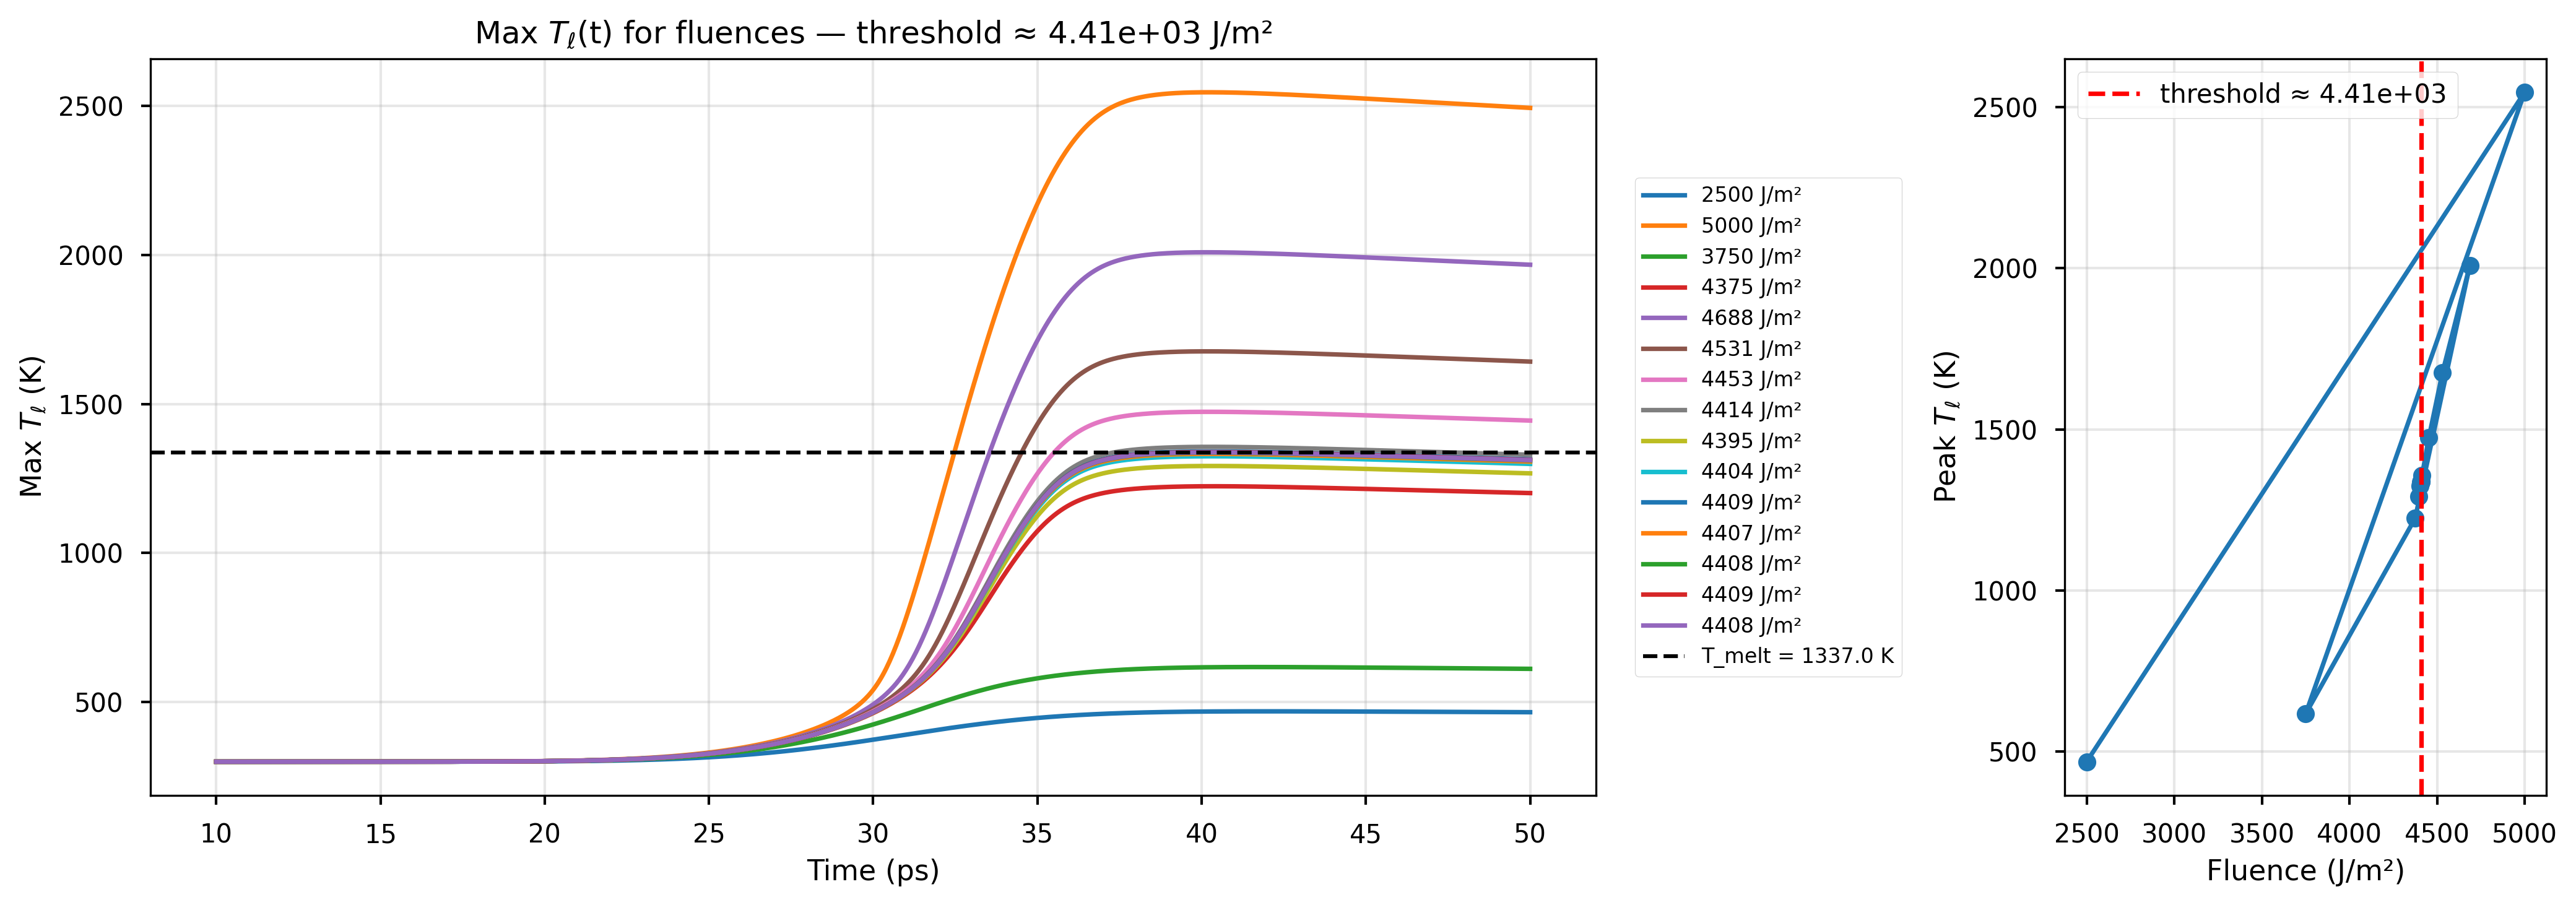
\includegraphics[width=0.47\linewidth]{figures/ch3/ablation_search_Au.png}
    }\hfill
    \subfloat[Au, 2D.\label{fig:ch3-ablation-linear-au-2d}]{%
        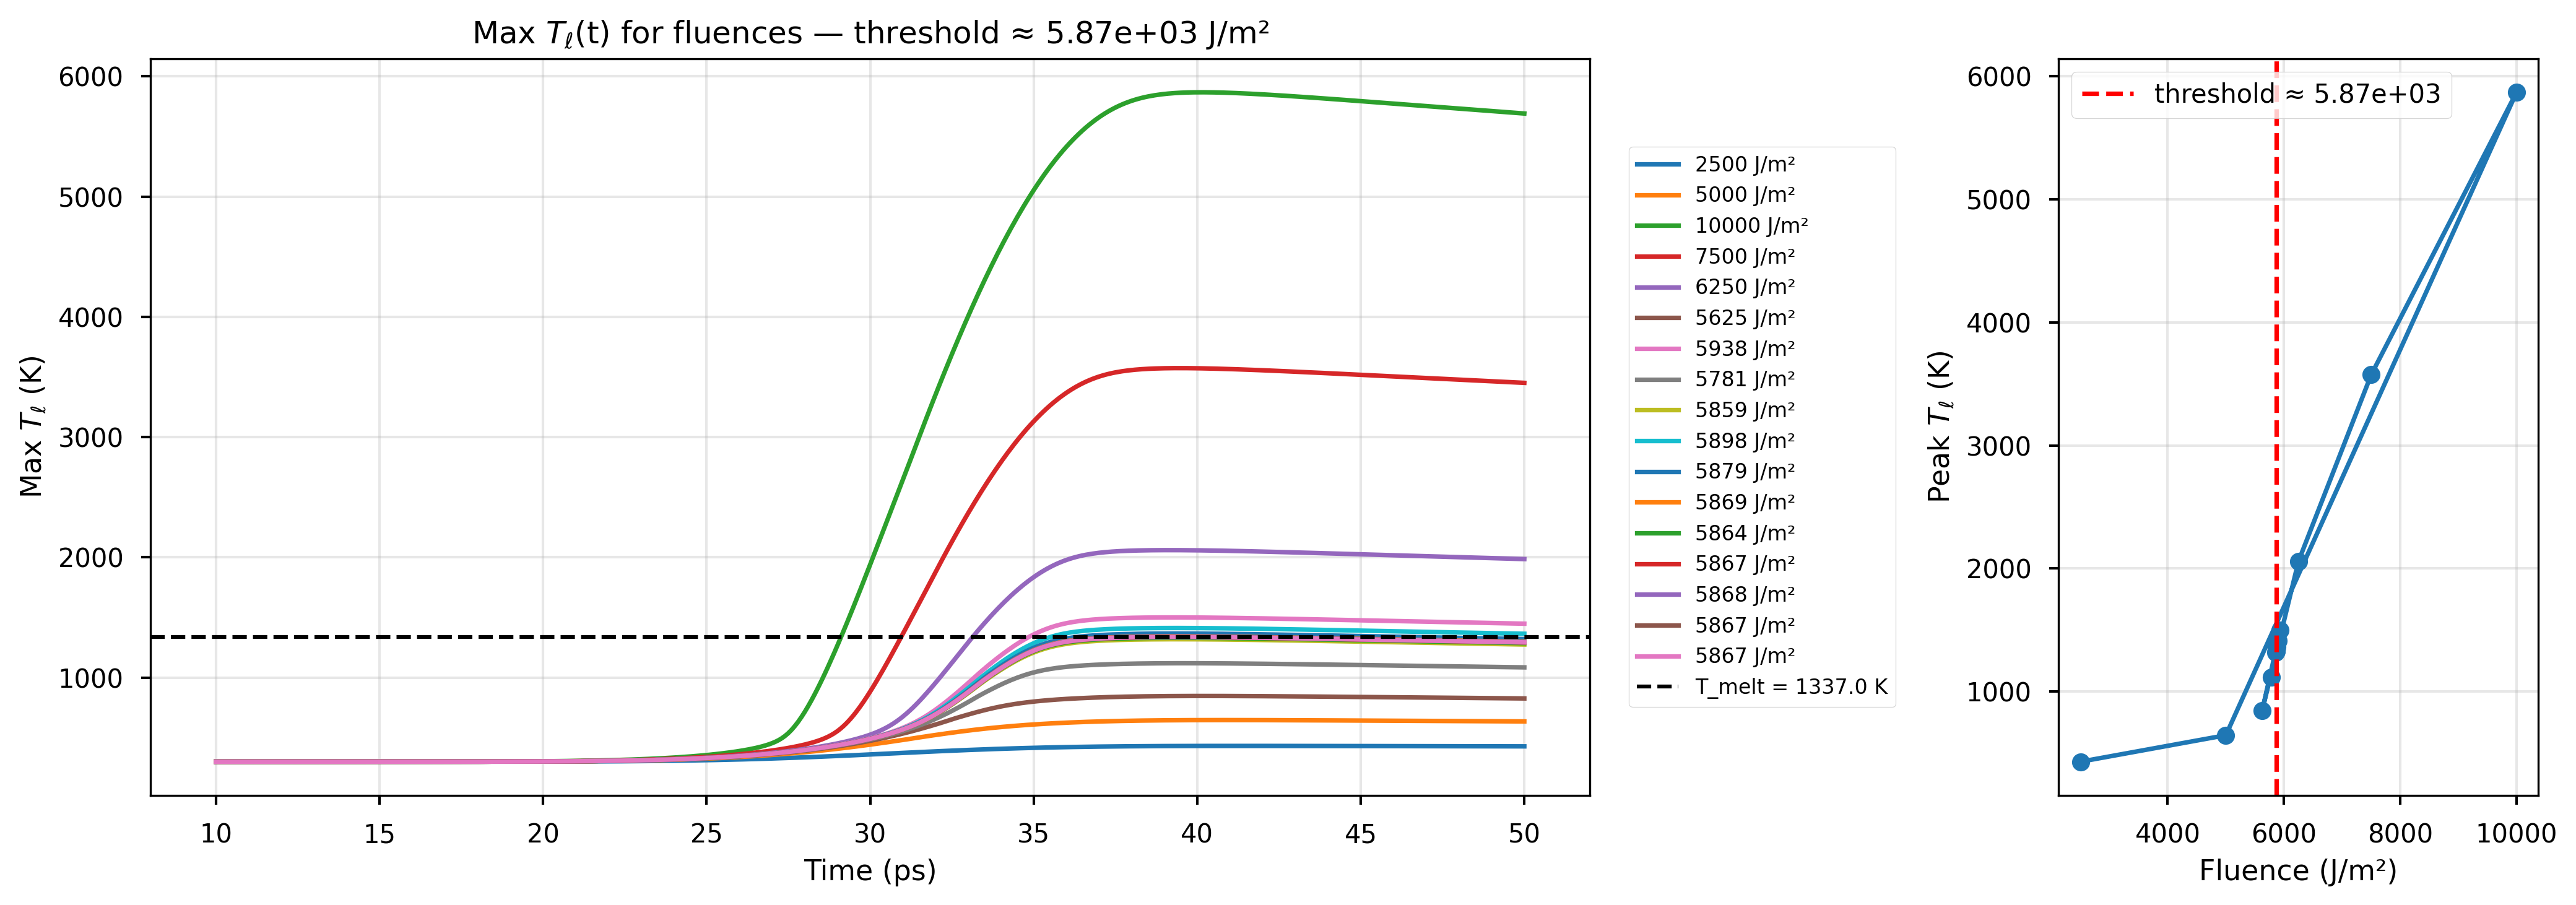
\includegraphics[width=0.47\linewidth]{figures/ch3/ablation_search_2d_Au.png}
    }\\[0.5em]
    \subfloat[Ni, 1D.\label{fig:ch3-ablation-linear-ni-1d}]{%
        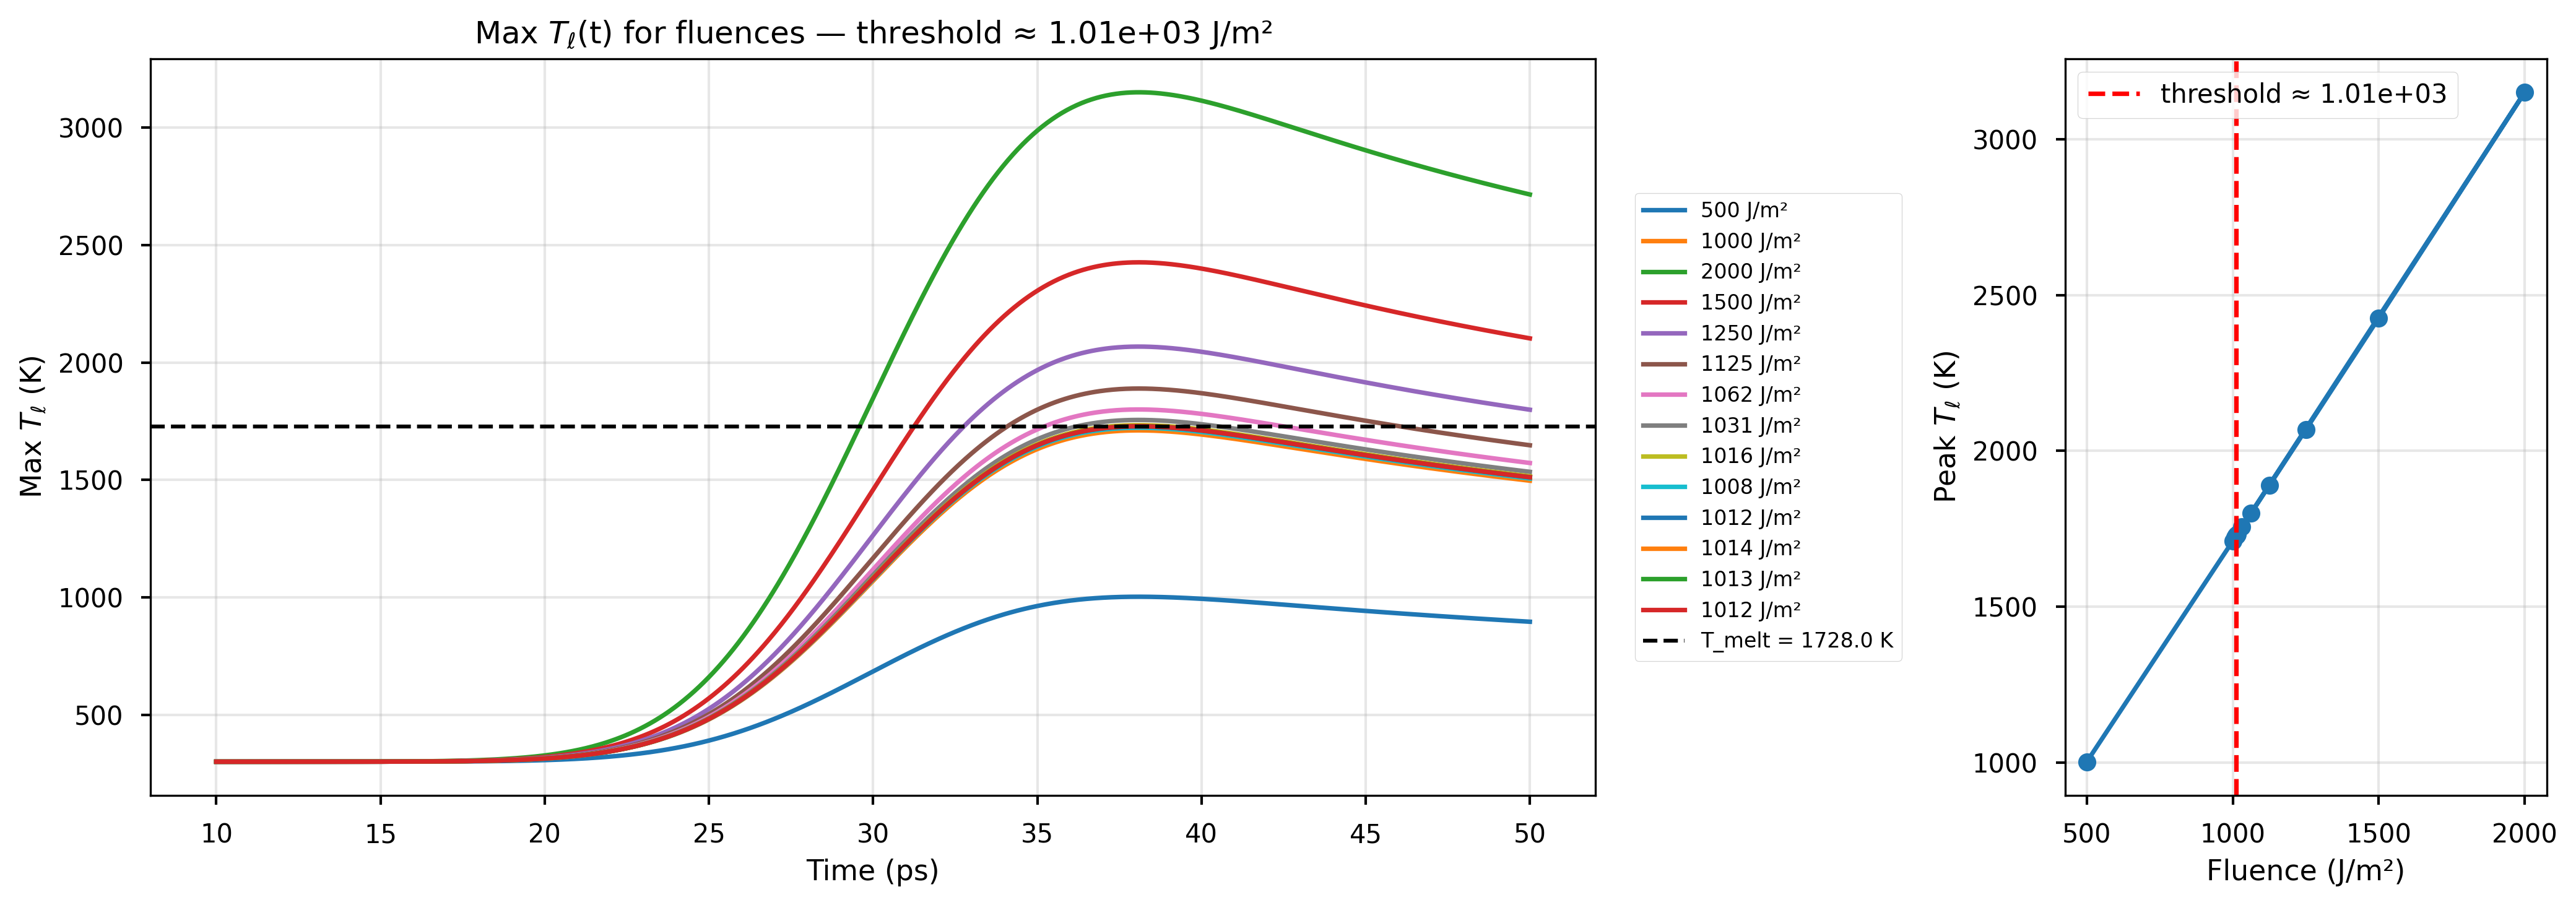
\includegraphics[width=0.47\linewidth]{figures/ch3/ablation_search_Ni.png}
    }\hfill
    \subfloat[Ni, 2D.\label{fig:ch3-ablation-linear-ni-2d}]{%
        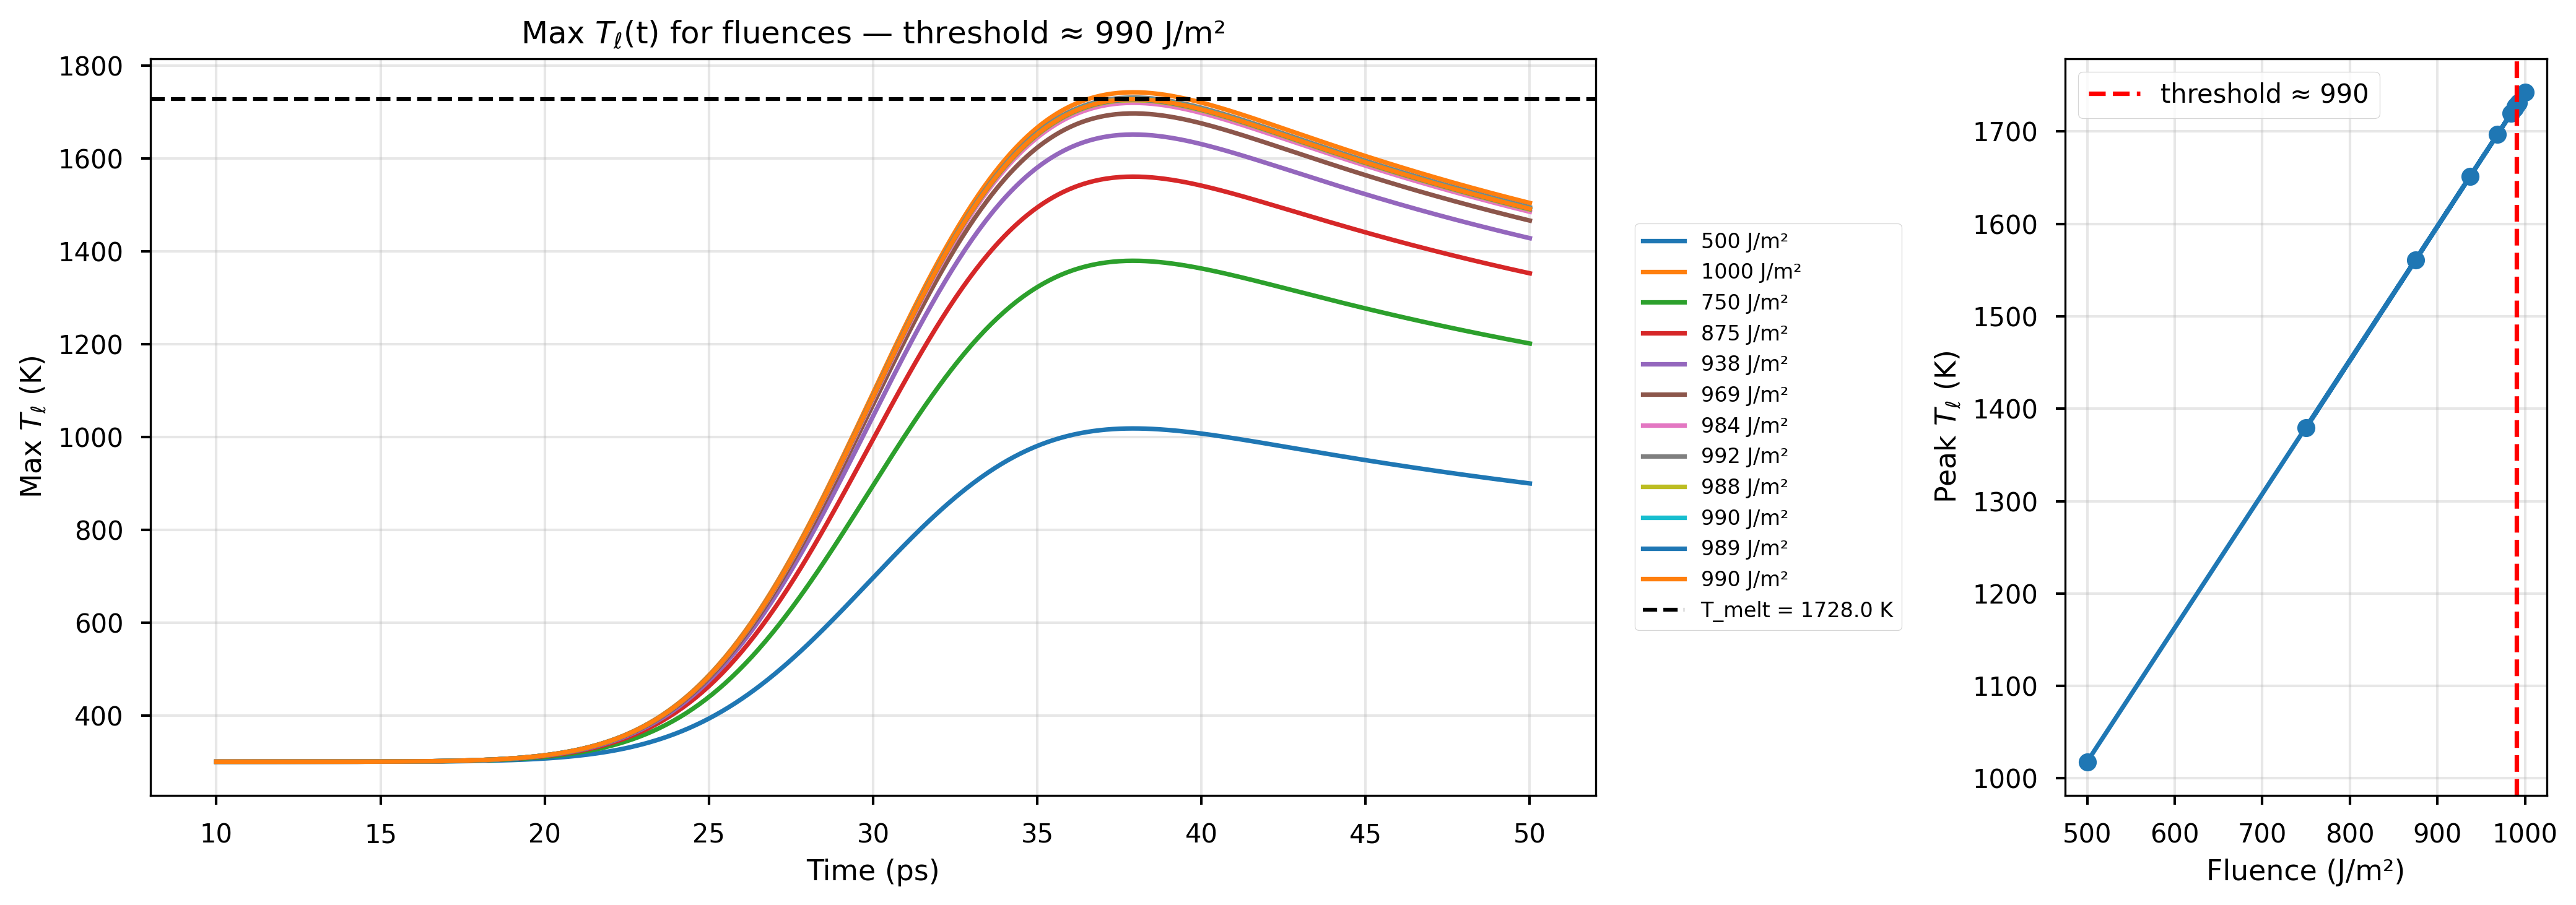
\includegraphics[width=0.47\linewidth]{figures/ch3/ablation_search_2d_Ni.png}
    }\\[0.5em]
    \subfloat[Cu, 1D.\label{fig:ch3-ablation-linear-cu-1d}]{%
        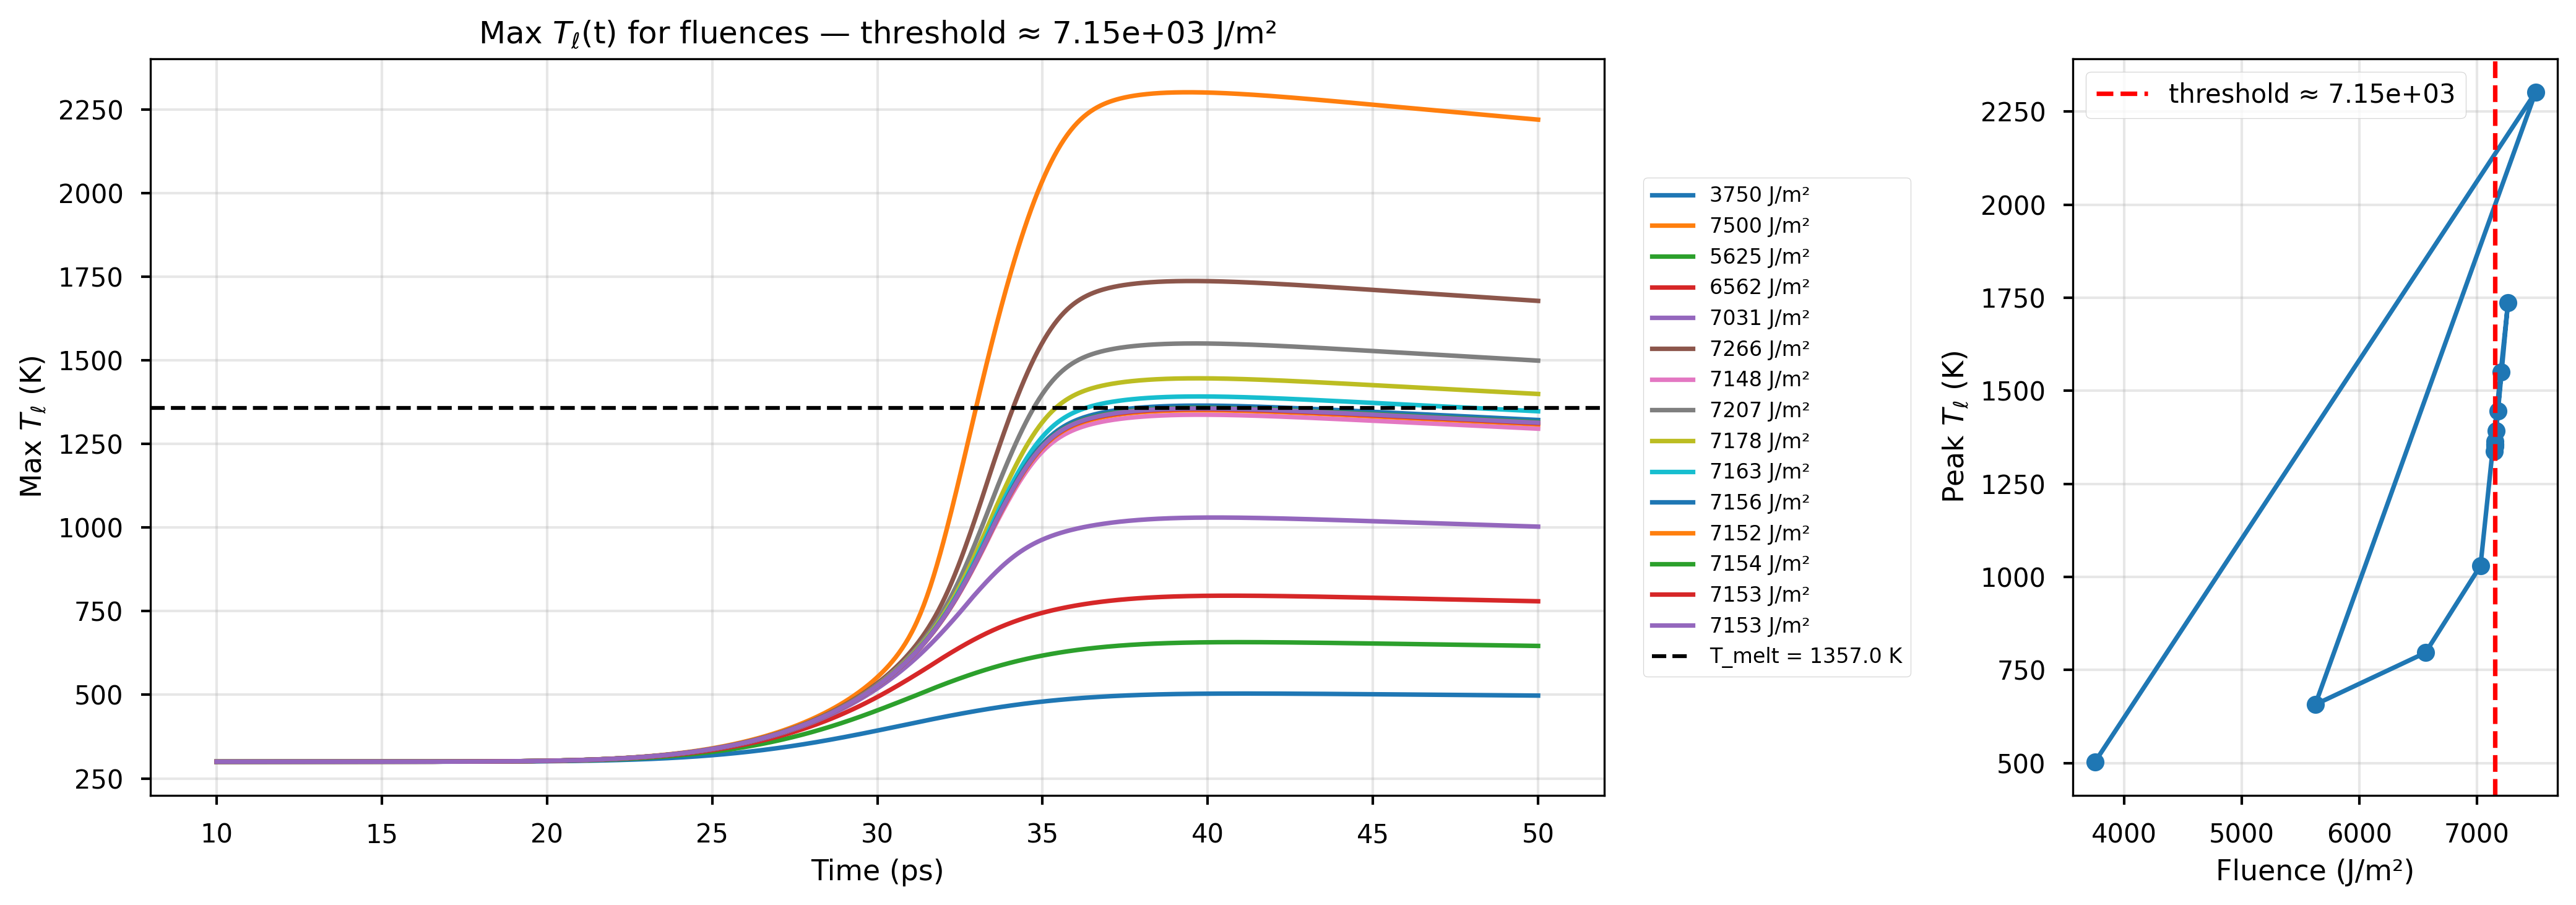
\includegraphics[width=0.47\linewidth]{figures/ch3/ablation_search_Cu.png}
    }\hfill
    \subfloat[Cu, 2D.\label{fig:ch3-ablation-linear-cu-2d}]{%
        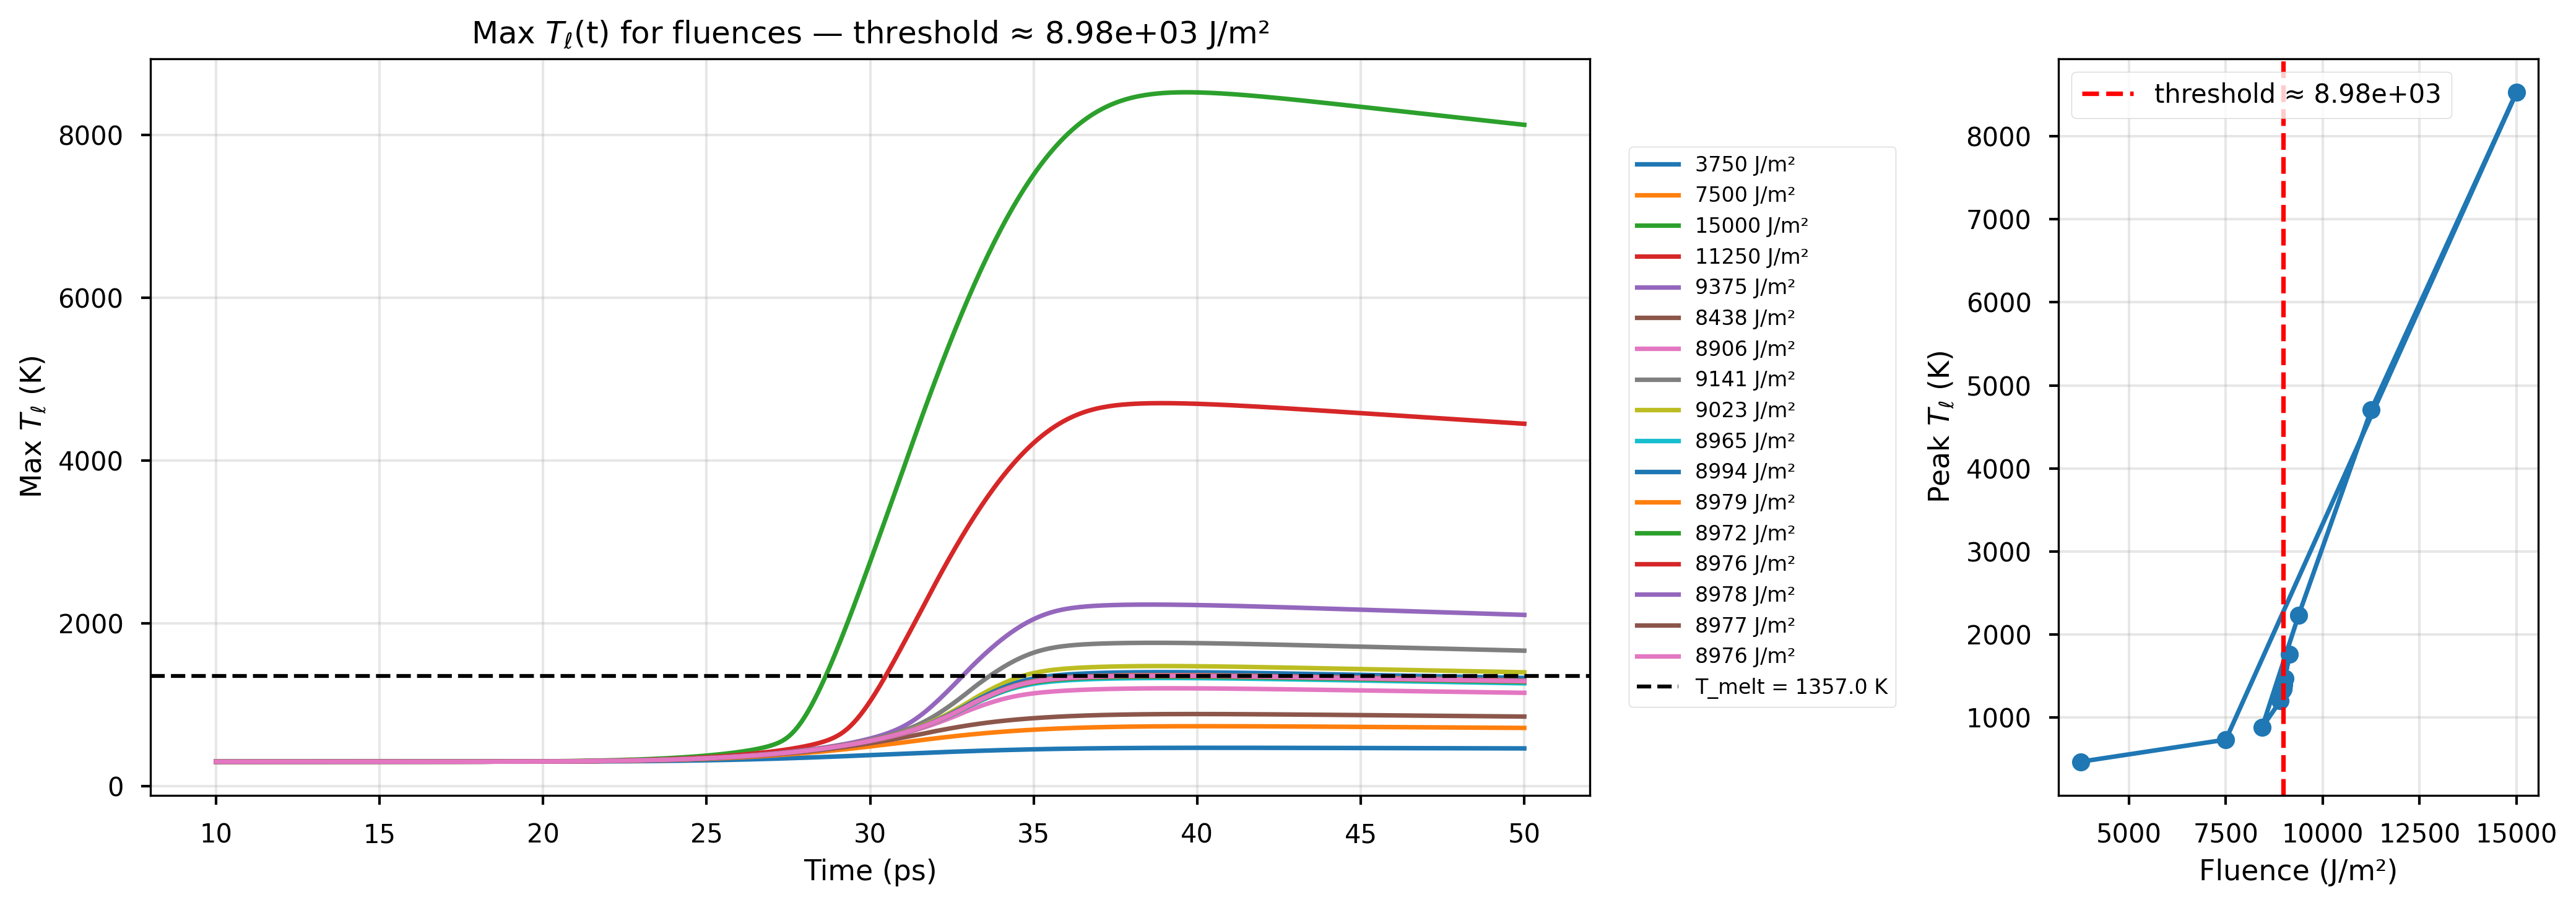
\includegraphics[width=0.47\linewidth]{figures/ch3/ablation_search_2d_Cu.png}
    }
    \caption{Ablation-threshold search results for Au, Ni, and Cu using the linear pTTM solver and the exponential--bisection algorithm. In each material/dimension case, the left panel shows the time history of \(T_{l,\max}(t)\) for the sampled trial fluences, while the right panel shows the corresponding peak value \(T_{l,\max}(F)\). The dashed horizontal line marks the melting temperature \(T_m\), and the vertical dashed line marks the estimated threshold \(\hat{F}_{\mathrm{th}}\).}
    \label{fig:ch3-ablation-linear}
\end{figure}

\subsubsection{Nonlinear pTTM thresholds}
\label{sec:ch3-ablation-nonlinear}

The nonlinear thresholds are listed in
Table~\ref{tab:ch3-threshold-nonlinear}, and the corresponding search
trajectories are shown in Fig.~\ref{fig:ch3-ablation-nonlinear}. As in the
linear case, the peak-temperature curves are monotone in the sampled
fluence range, so the bracketing assumptions remain compatible with the
observed numerical data.

The same dimensional trend persists, but with different magnitudes. For
Au, the 2D nonlinear threshold exceeds the 1D threshold by
\(\SI{2174.69}{\joule\per\square\metre}\), i.e.\ about \(23.7\%\). For
Cu, the increase is \(\SI{2050.76}{\joule\per\square\metre}\), i.e.\
about \(16.7\%\). For Ni, the 2D and 1D thresholds again remain extremely
close, with a small decrease of \(\SI{8.79}{\joule\per\square\metre}\)
(\(0.7\%\)) in 2D.

\begin{table}[htbp]
    \centering
    \caption{
    Nonlinear pTTM threshold estimates obtained with exponential bracketing and bisection refinement.
    Fluence values \(F_{\mathrm{init}}\), \(\hat{F}_{\mathrm{th}}\), and \(\delta F_{\mathrm{bis}}\) are in \(\si{\joule\per\square\metre}\).
    }
    \label{tab:ch3-threshold-nonlinear}
    \begin{tabular}{@{}llccccl@{}}
        \toprule
        \rowcolor{gray!20}
        \textbf{Material}   & \textbf{Dim.} & \(\boldsymbol{F_{\mathrm{init}}}\) & \(\boldsymbol{\hat{F}_{\mathrm{th}}}\) & \(\boldsymbol{\delta F_{\mathrm{bis}}}\) & \(\boldsymbol{\hat{F}_{\mathrm{th}} \pm \delta F_{\mathrm{bis}}}\) (\(\si{\joule\per\square\centi\metre}\)) & \textbf{Runtime} \\
        \midrule
        \multirow{2}{*}{Au} & 1D            & 2500.00                            & 9192.81                                & 0.15                                     & \(0.919281 \pm 0.000015\)                                                                                   & 5m 47.9s         \\
                            & 2D            & 2500.00                            & 11367.50                               & 0.15                                     & \(1.136750 \pm 0.000015\)                                                                                   & 2h 28m 06s       \\
        \midrule
        \multirow{2}{*}{Ni} & 1D            & 500.00                             & 1276.86                                & 0.24                                     & \(0.127686 \pm 0.000024\)                                                                                   & 4m 37.7s         \\
                            & 2D            & 500.00                             & 1268.07                                & 0.24                                     & \(0.126807 \pm 0.000024\)                                                                                   & 1h 40m 19s       \\
        \midrule
        \multirow{2}{*}{Cu} & 1D            & 3750.00                            & 12260.30                               & 0.23                                     & \(1.226030 \pm 0.000023\)                                                                                   & 5m 41.2s         \\
                            & 2D            & 3750.00                            & 14311.06                               & 0.23                                     & \(1.431106 \pm 0.000023\)                                                                                   & 2h 18m 37s       \\
        \bottomrule
    \end{tabular}
\end{table}

\begin{figure}[H]
    \centering
    \subfloat[Au, 1D.\label{fig:ch3-ablation-nl-au-1d}]{%
        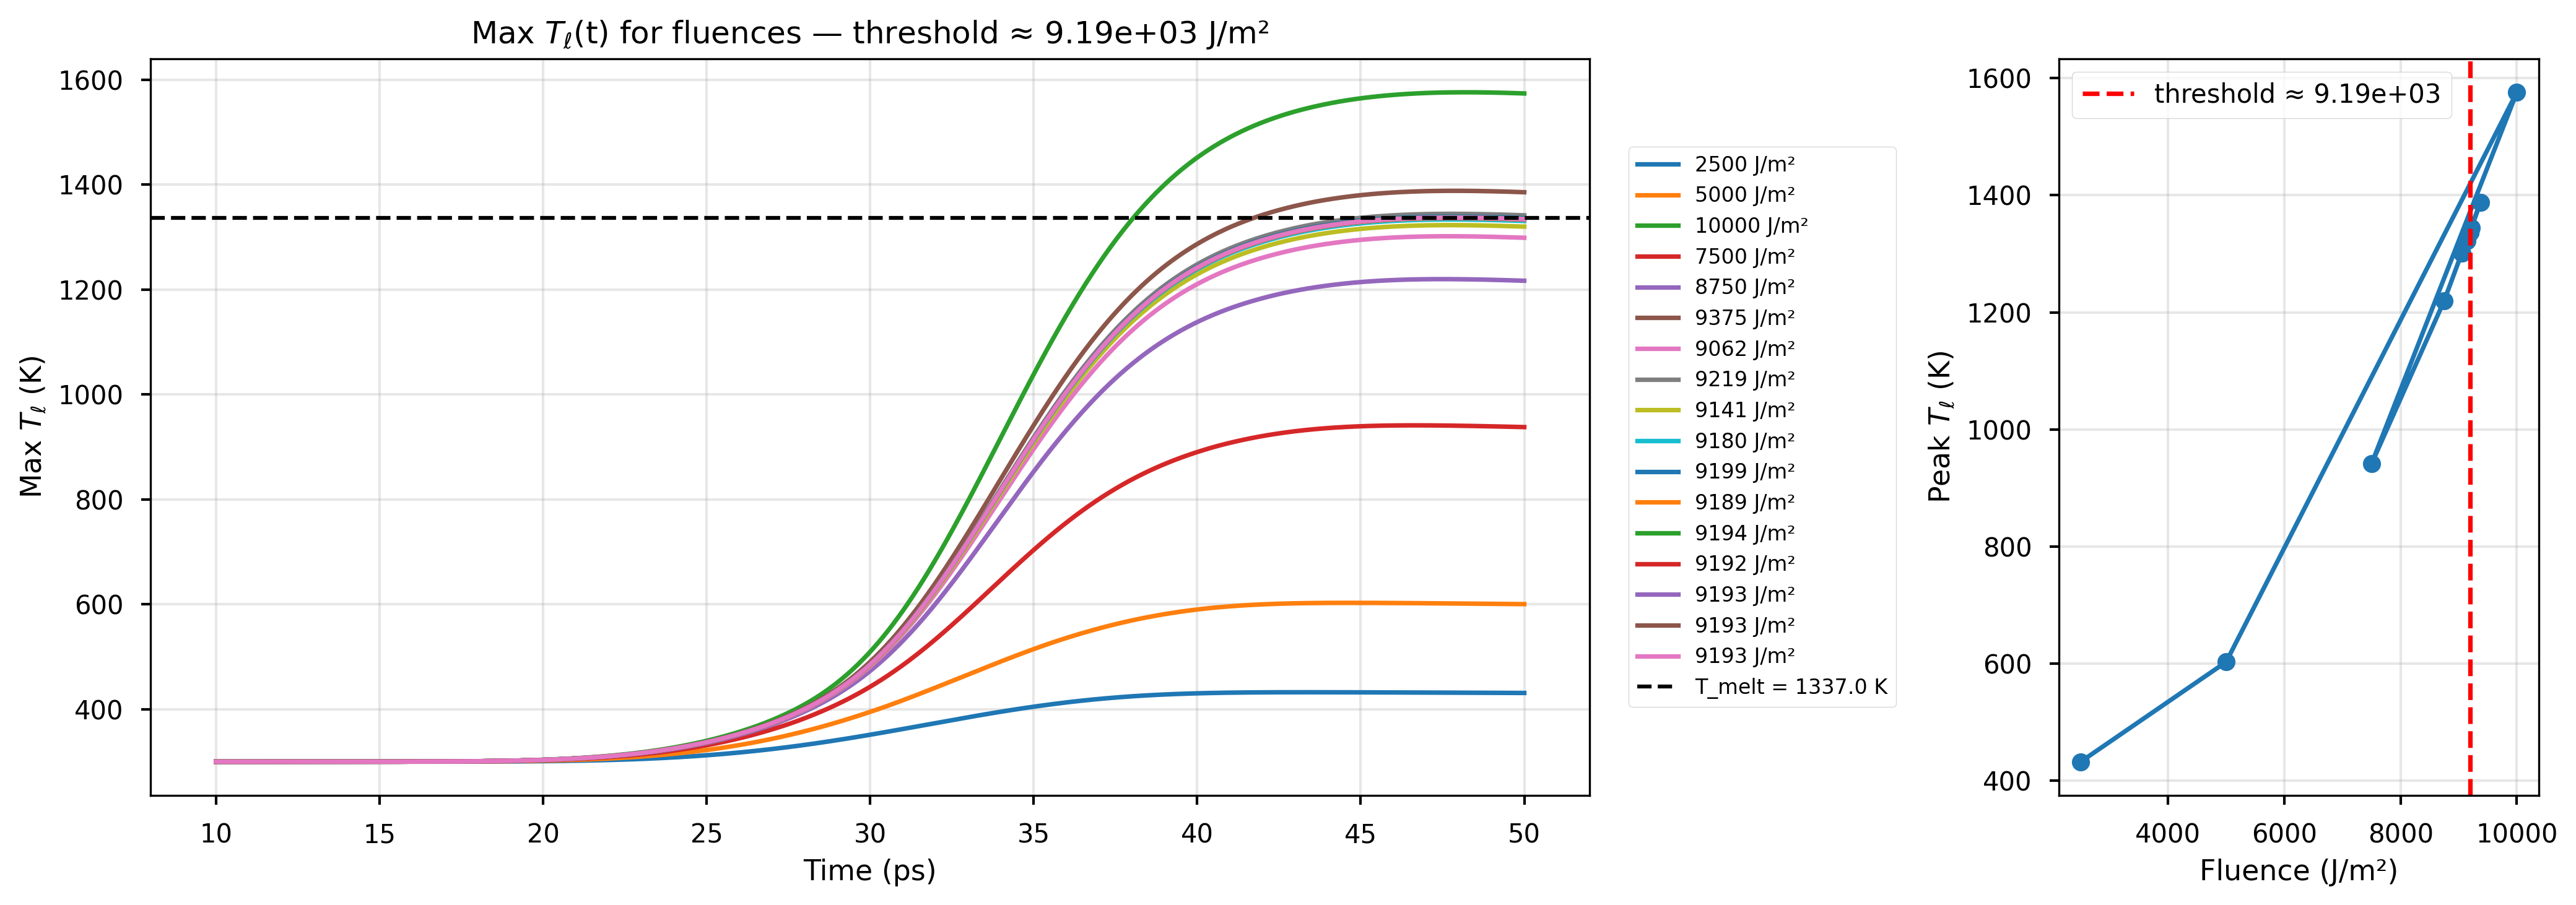
\includegraphics[width=0.47\linewidth]{figures/ch3/ablation_search_nl_Au.png}
    }\hfill
    \subfloat[Au, 2D.\label{fig:ch3-ablation-nl-au-2d}]{%
        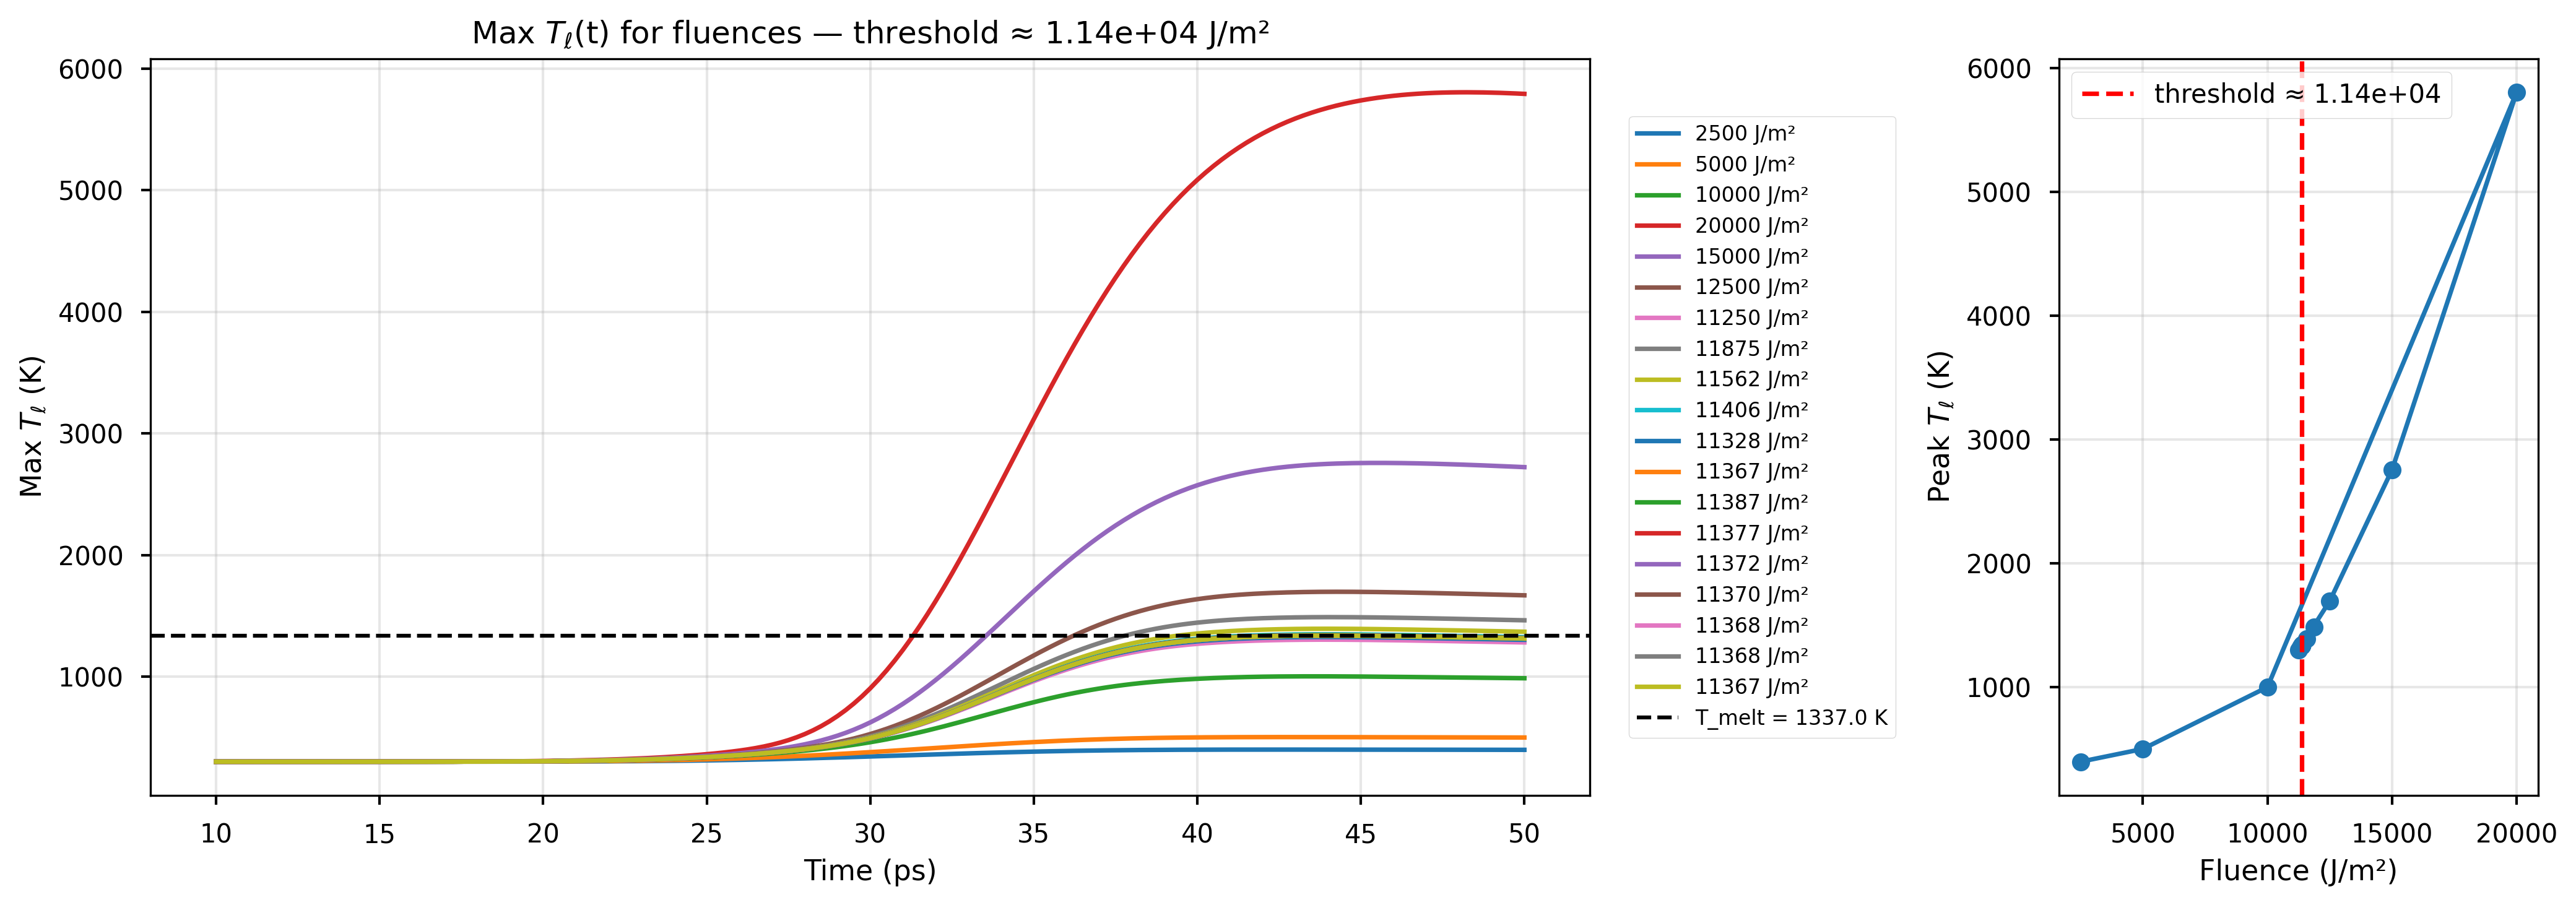
\includegraphics[width=0.47\linewidth]{figures/ch3/ablation_search_2d_nl_Au.png}
    }\\[0.5em]
    \subfloat[Ni, 1D.\label{fig:ch3-ablation-nl-ni-1d}]{%
        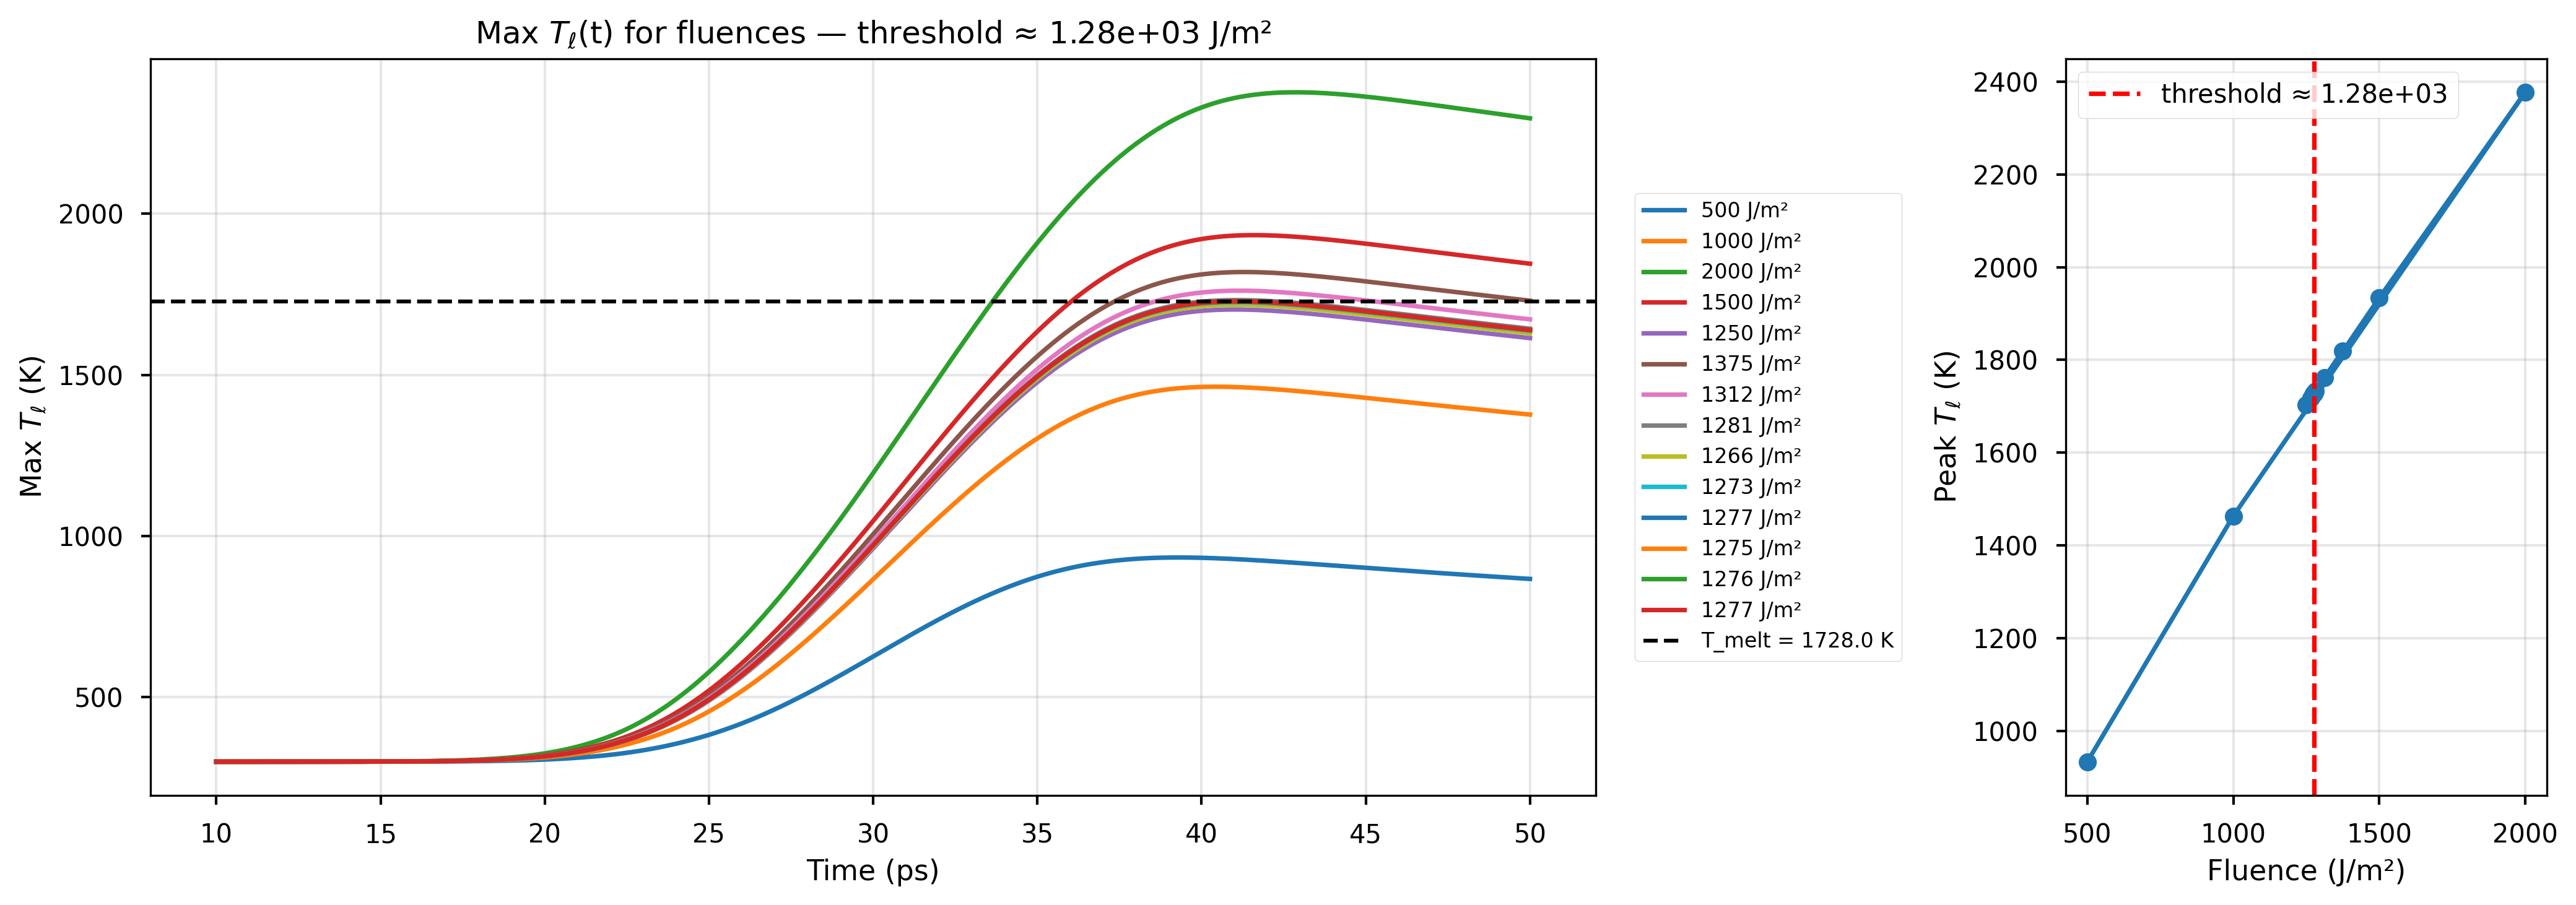
\includegraphics[width=0.47\linewidth]{figures/ch3/ablation_search_nl_Ni.png}
    }\hfill
    \subfloat[Ni, 2D.\label{fig:ch3-ablation-nl-ni-2d}]{%
        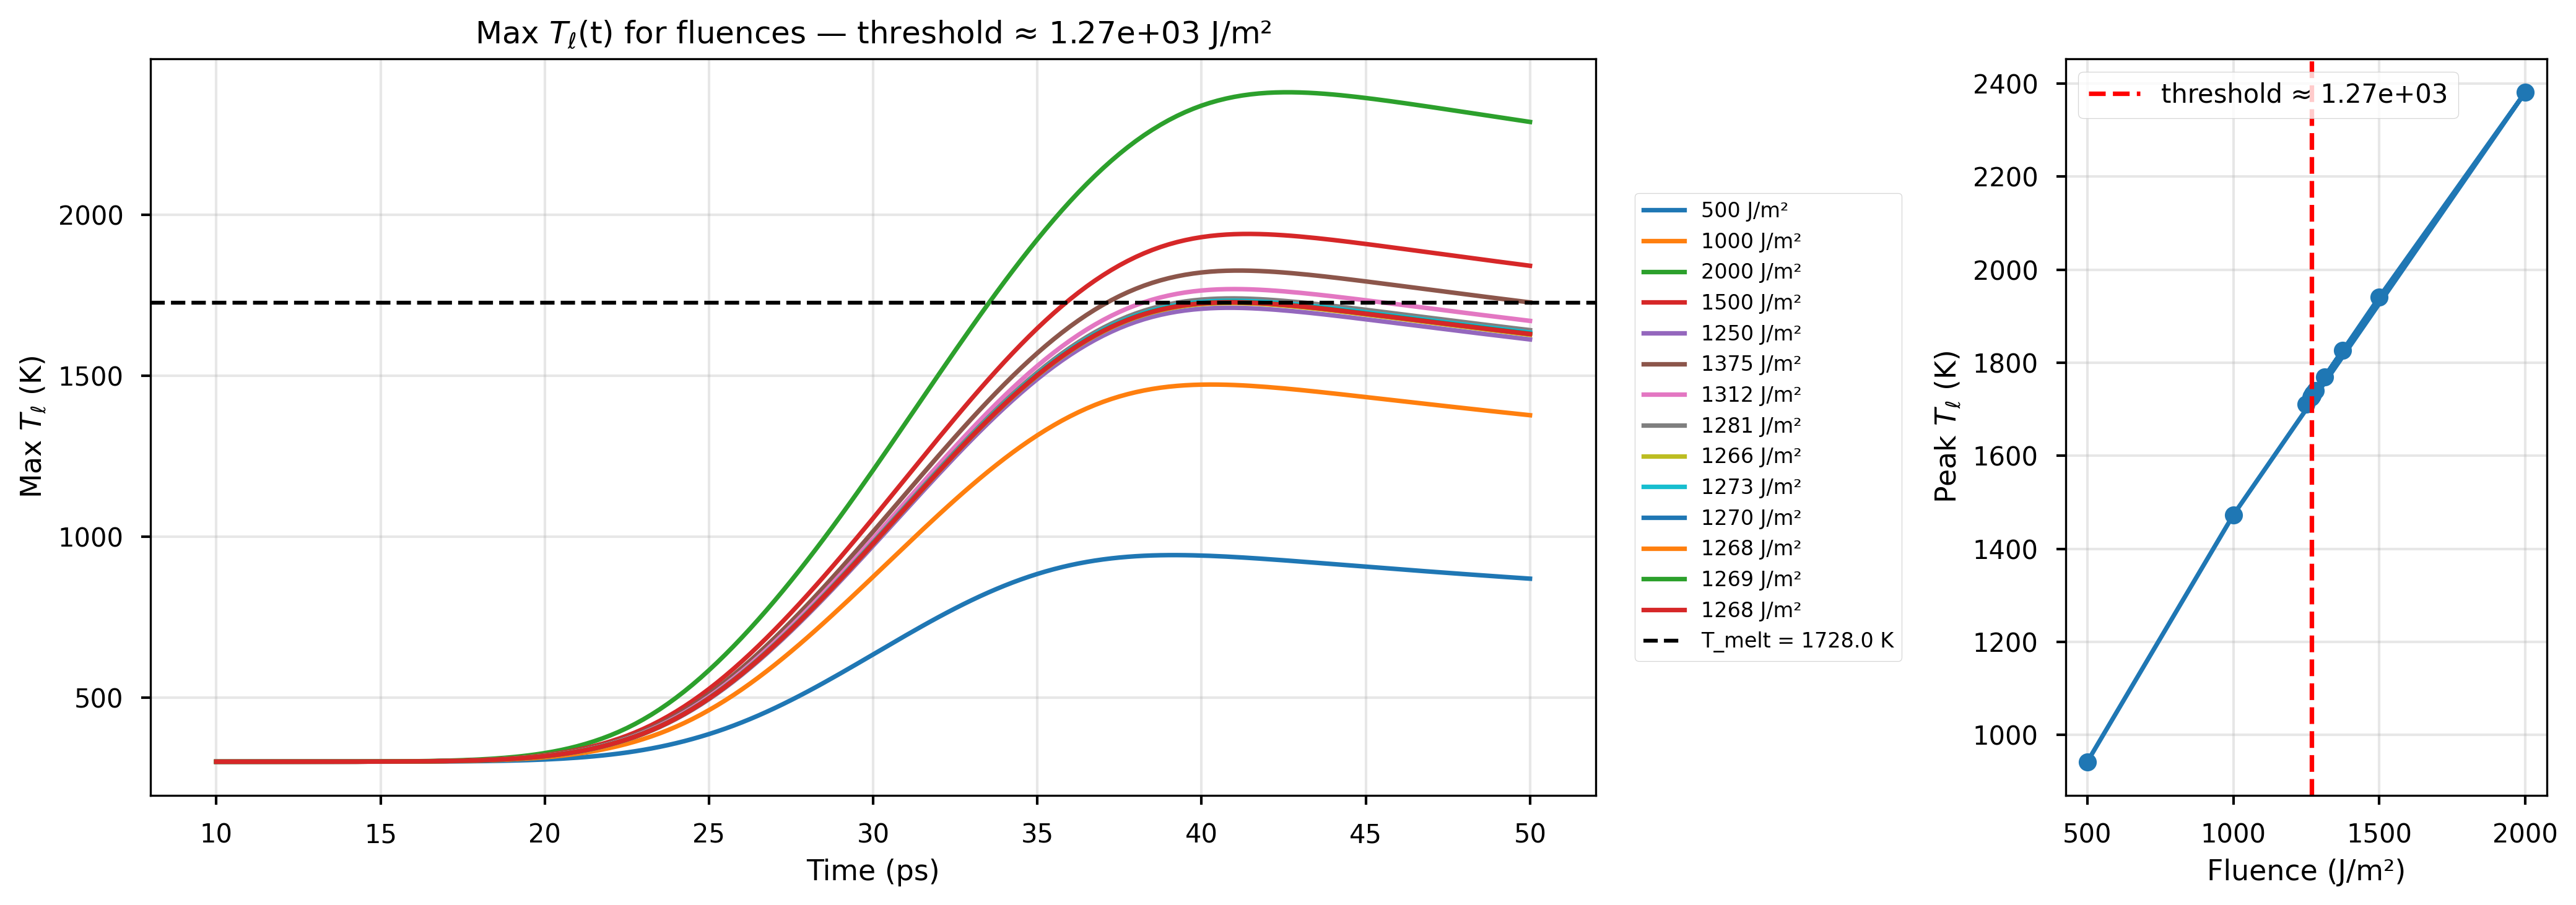
\includegraphics[width=0.47\linewidth]{figures/ch3/ablation_search_2d_nl_Ni.png}
    }\\[0.5em]
    \subfloat[Cu, 1D.\label{fig:ch3-ablation-nl-cu-1d}]{%
        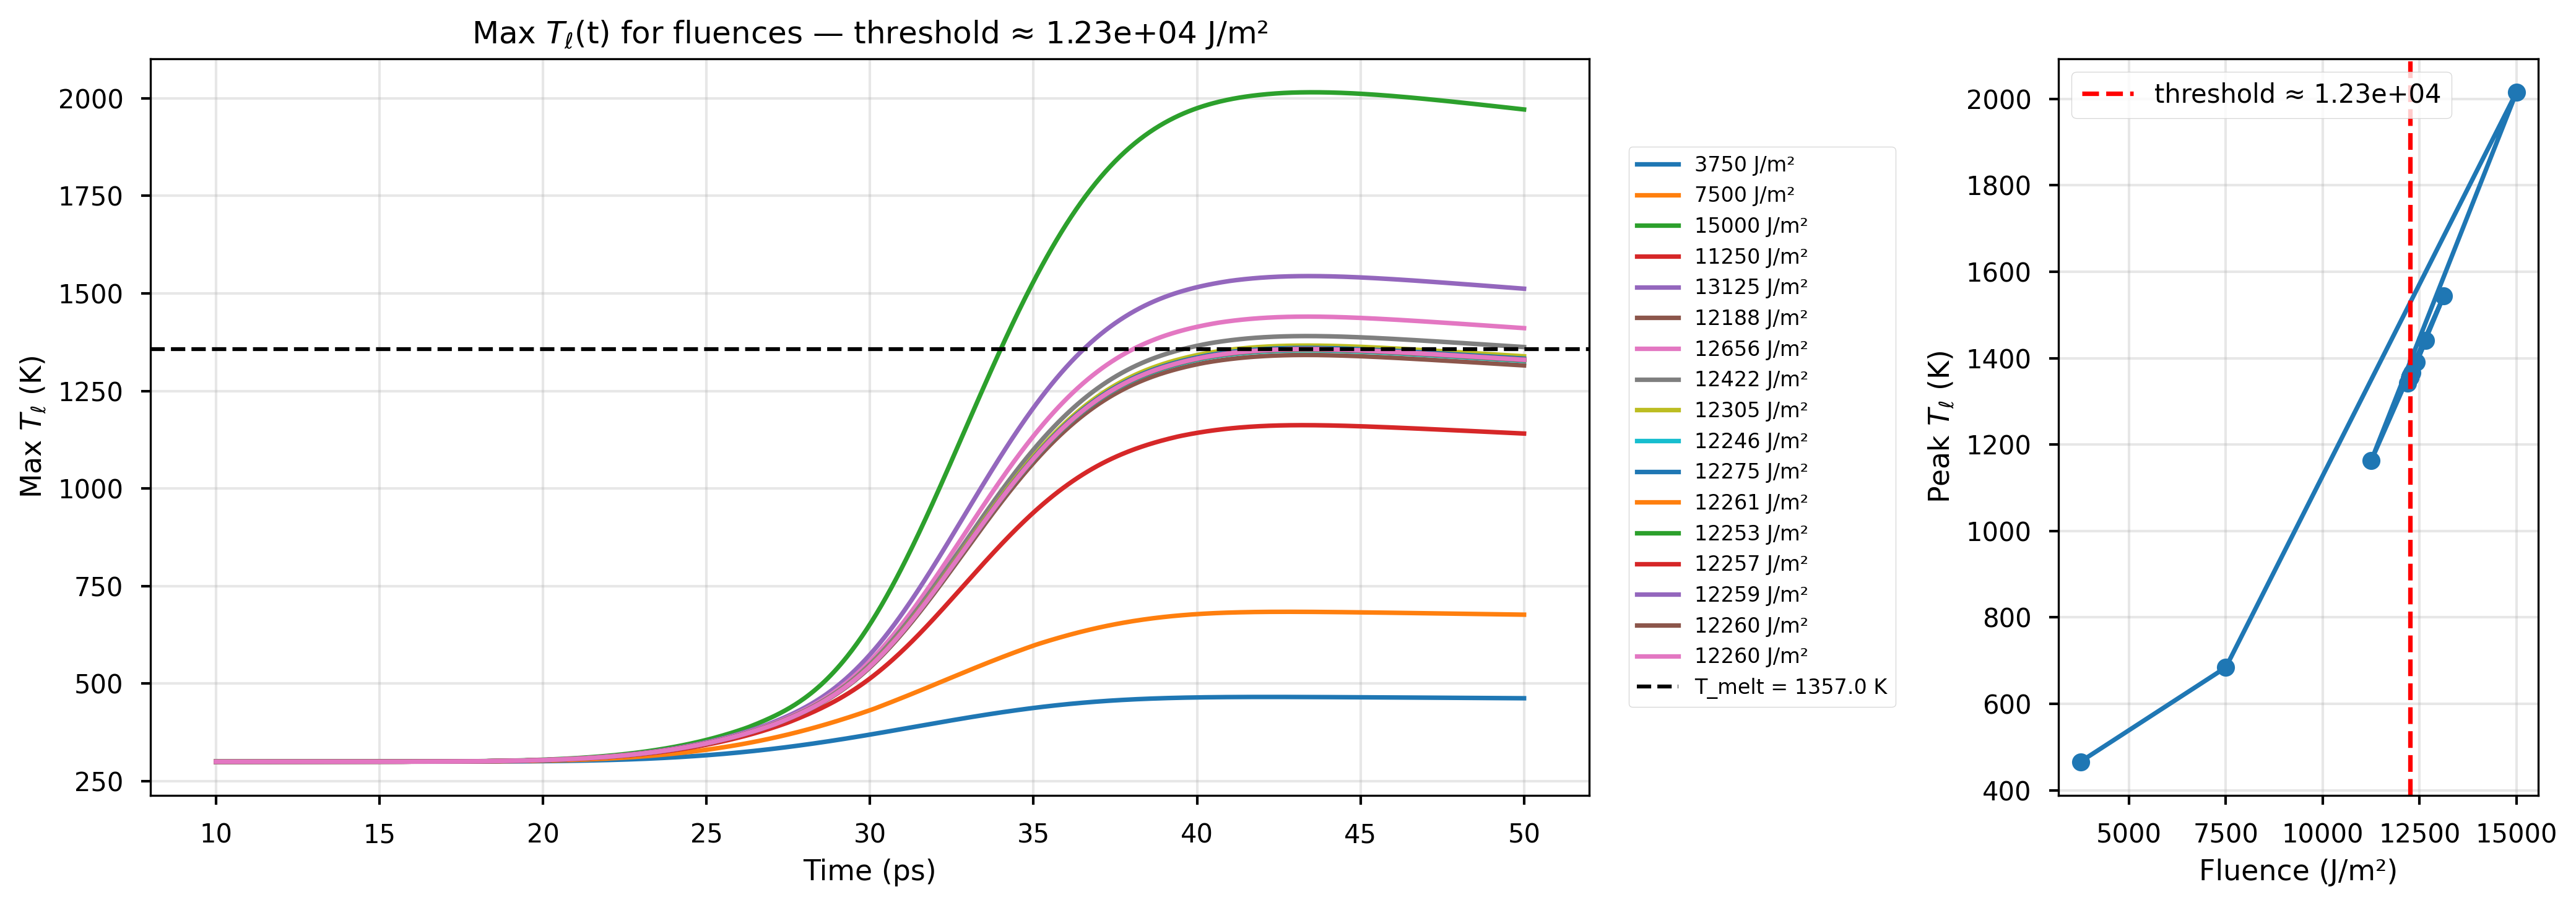
\includegraphics[width=0.47\linewidth]{figures/ch3/ablation_search_nl_Cu.png}
    }\hfill
    \subfloat[Cu, 2D.\label{fig:ch3-ablation-nl-cu-2d}]{%
        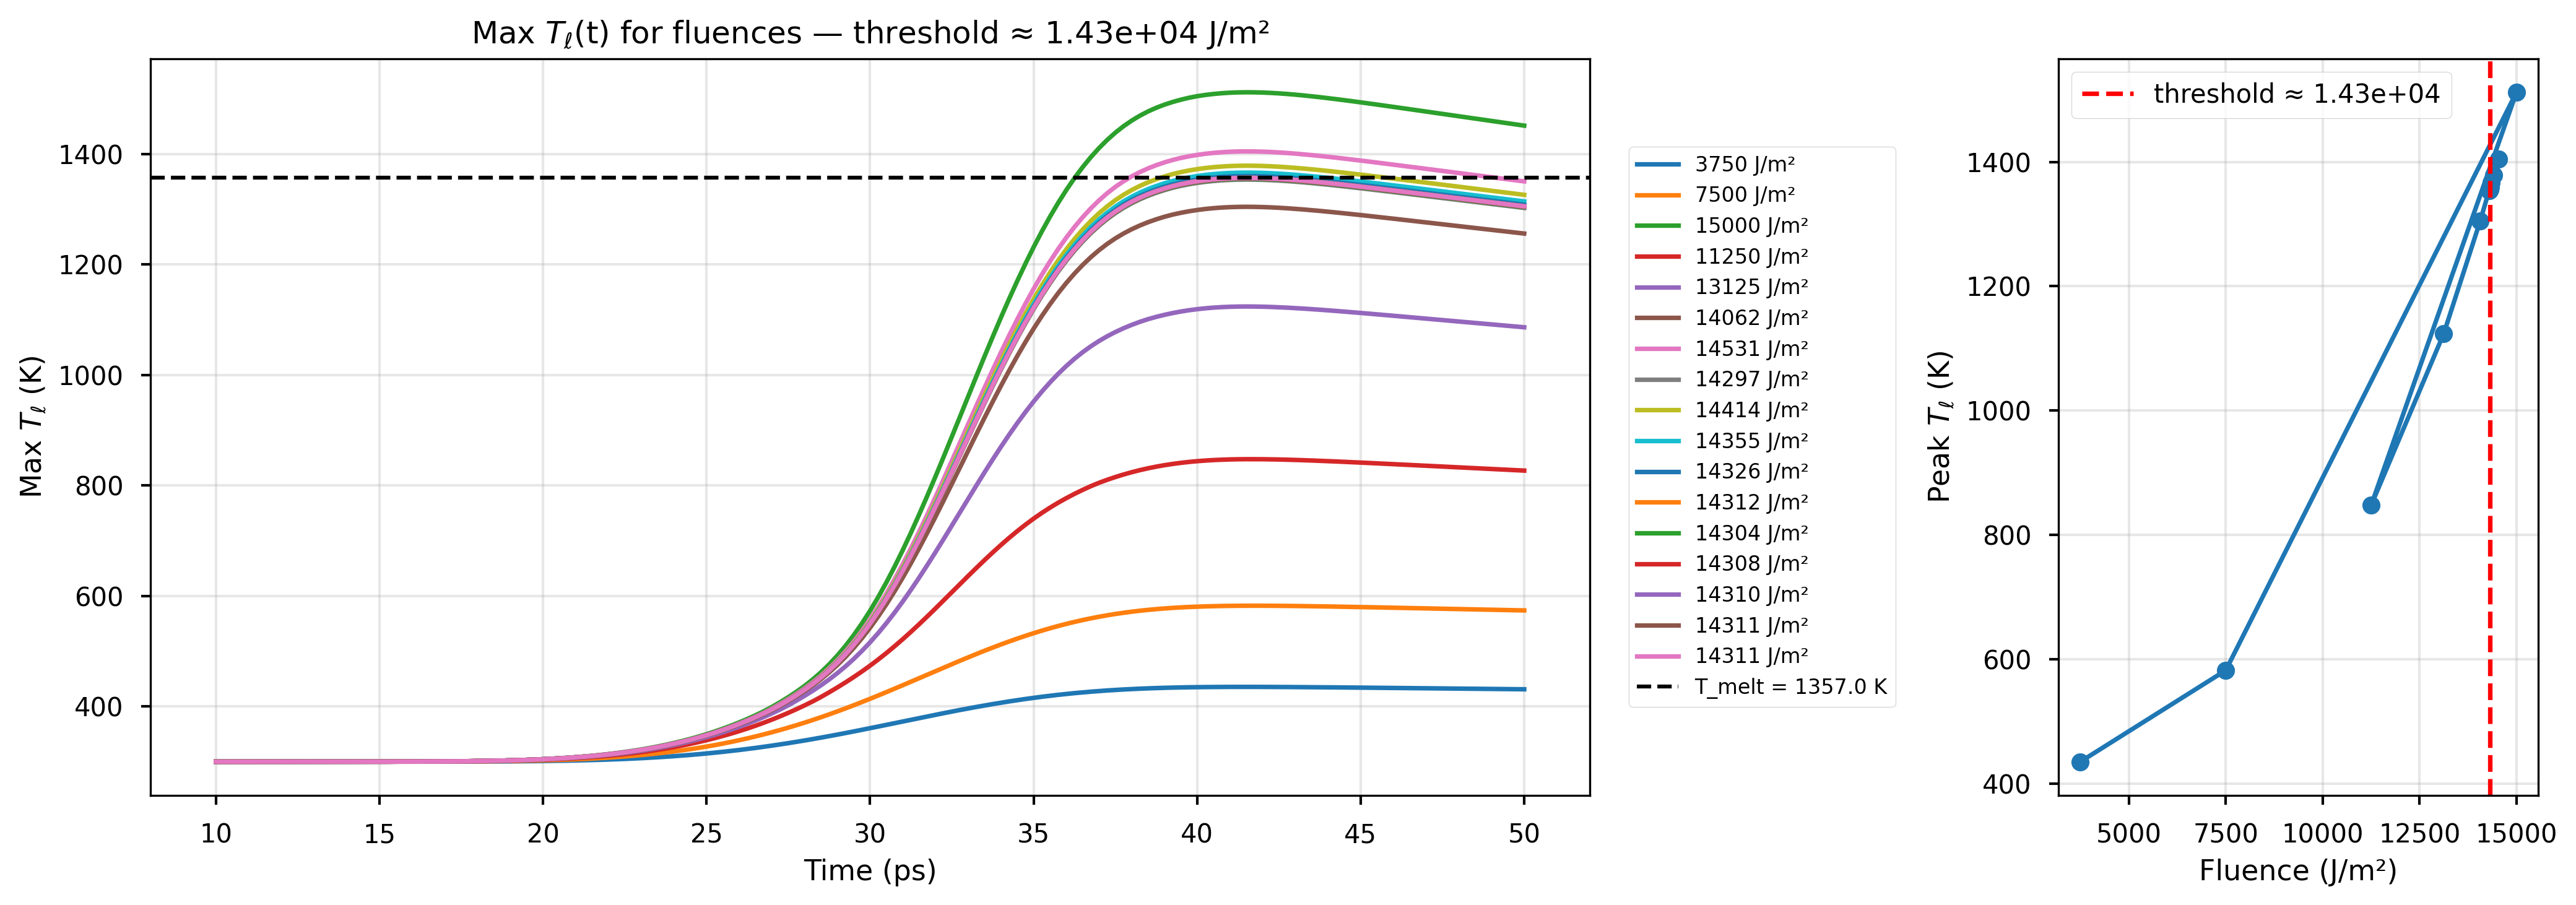
\includegraphics[width=0.47\linewidth]{figures/ch3/ablation_search_2d_nl_Cu.png}
    }
    \caption{Ablation-threshold search results for Au, Ni, and Cu using the nonlinear pTTM solver and the exponential--bisection algorithm. The interpretation of the panels is the same as in Fig.~\ref{fig:ch3-ablation-linear}.}
    \label{fig:ch3-ablation-nonlinear}
\end{figure}

\subsection{Comparative analysis and discussion}
\label{sec:ch3-ablation-discussion}

The threshold tables and the comparison plots lead to two robust
conclusions. First, the dimensionality effect is strongly
material-dependent: moving from 1D to 2D substantially increases the
threshold for Au and Cu, but leaves Ni almost unchanged. Second, and more
importantly for model selection, the nonlinear constitutive model raises
the predicted threshold for all three materials and in both dimensions.
Thus, near melting onset, the linear pTTM is not an accurate surrogate for
the nonlinear model.

\subsubsection{One-dimensional versus two-dimensional predictions}
\label{sec:ch3-ablation-discussion-1d2d}

Figures~\ref{fig:ch3-1d-2d-comparison-linear-metals} and
\ref{fig:ch3-1d-2d-comparison-nonlinear-metals} compare the 1D and 2D
surface lattice-temperature histories at a common fluence. In the 1D
curves, the representative signal is \(T_l(z_s,t)\). In the 2D curves, it
is the surface maximum \(\max_x T_l(x,z_s,t)\), which is the quantity most
relevant to the melting-onset criterion used in the threshold search.

For Au and Cu, the 2D response lies below the corresponding 1D response in
both the linear and nonlinear settings during the main heating window.
This appears clearly in the lower panels of
Figs.~\ref{fig:ch3-1d-2d-comparison-linear-metals} and
\ref{fig:ch3-1d-2d-comparison-nonlinear-metals}, where the quantity
\(\Delta T_l(t) = T_l^{\mathrm{2D}} - T_l^{\mathrm{1D}}\) is negative by
several hundred kelvin near the peak. Consequently, a larger incident
fluence is required in 2D to reach \(T_m\), which explains the higher 2D
thresholds for Au and Cu.

Ni behaves differently. In both the linear and nonlinear comparisons, the
1D and 2D curves remain close and the difference changes sign over time.
Near the peak-heating interval, the 2D surface maximum is slightly above
the 1D value, which is consistent with the small negative threshold
difference \(F_{\mathrm{th}}^{\mathrm{2D}}-F_{\mathrm{th}}^{\mathrm{1D}}\)
reported in Tables~\ref{tab:ch3-threshold-linear} and
\ref{tab:ch3-threshold-nonlinear}. The dimensional reduction is therefore
not uniformly conservative across materials.

\begin{figure}[H]
    \centering
    \subfloat[Au.\label{fig:ch3-comparison-linear-au}]{%
        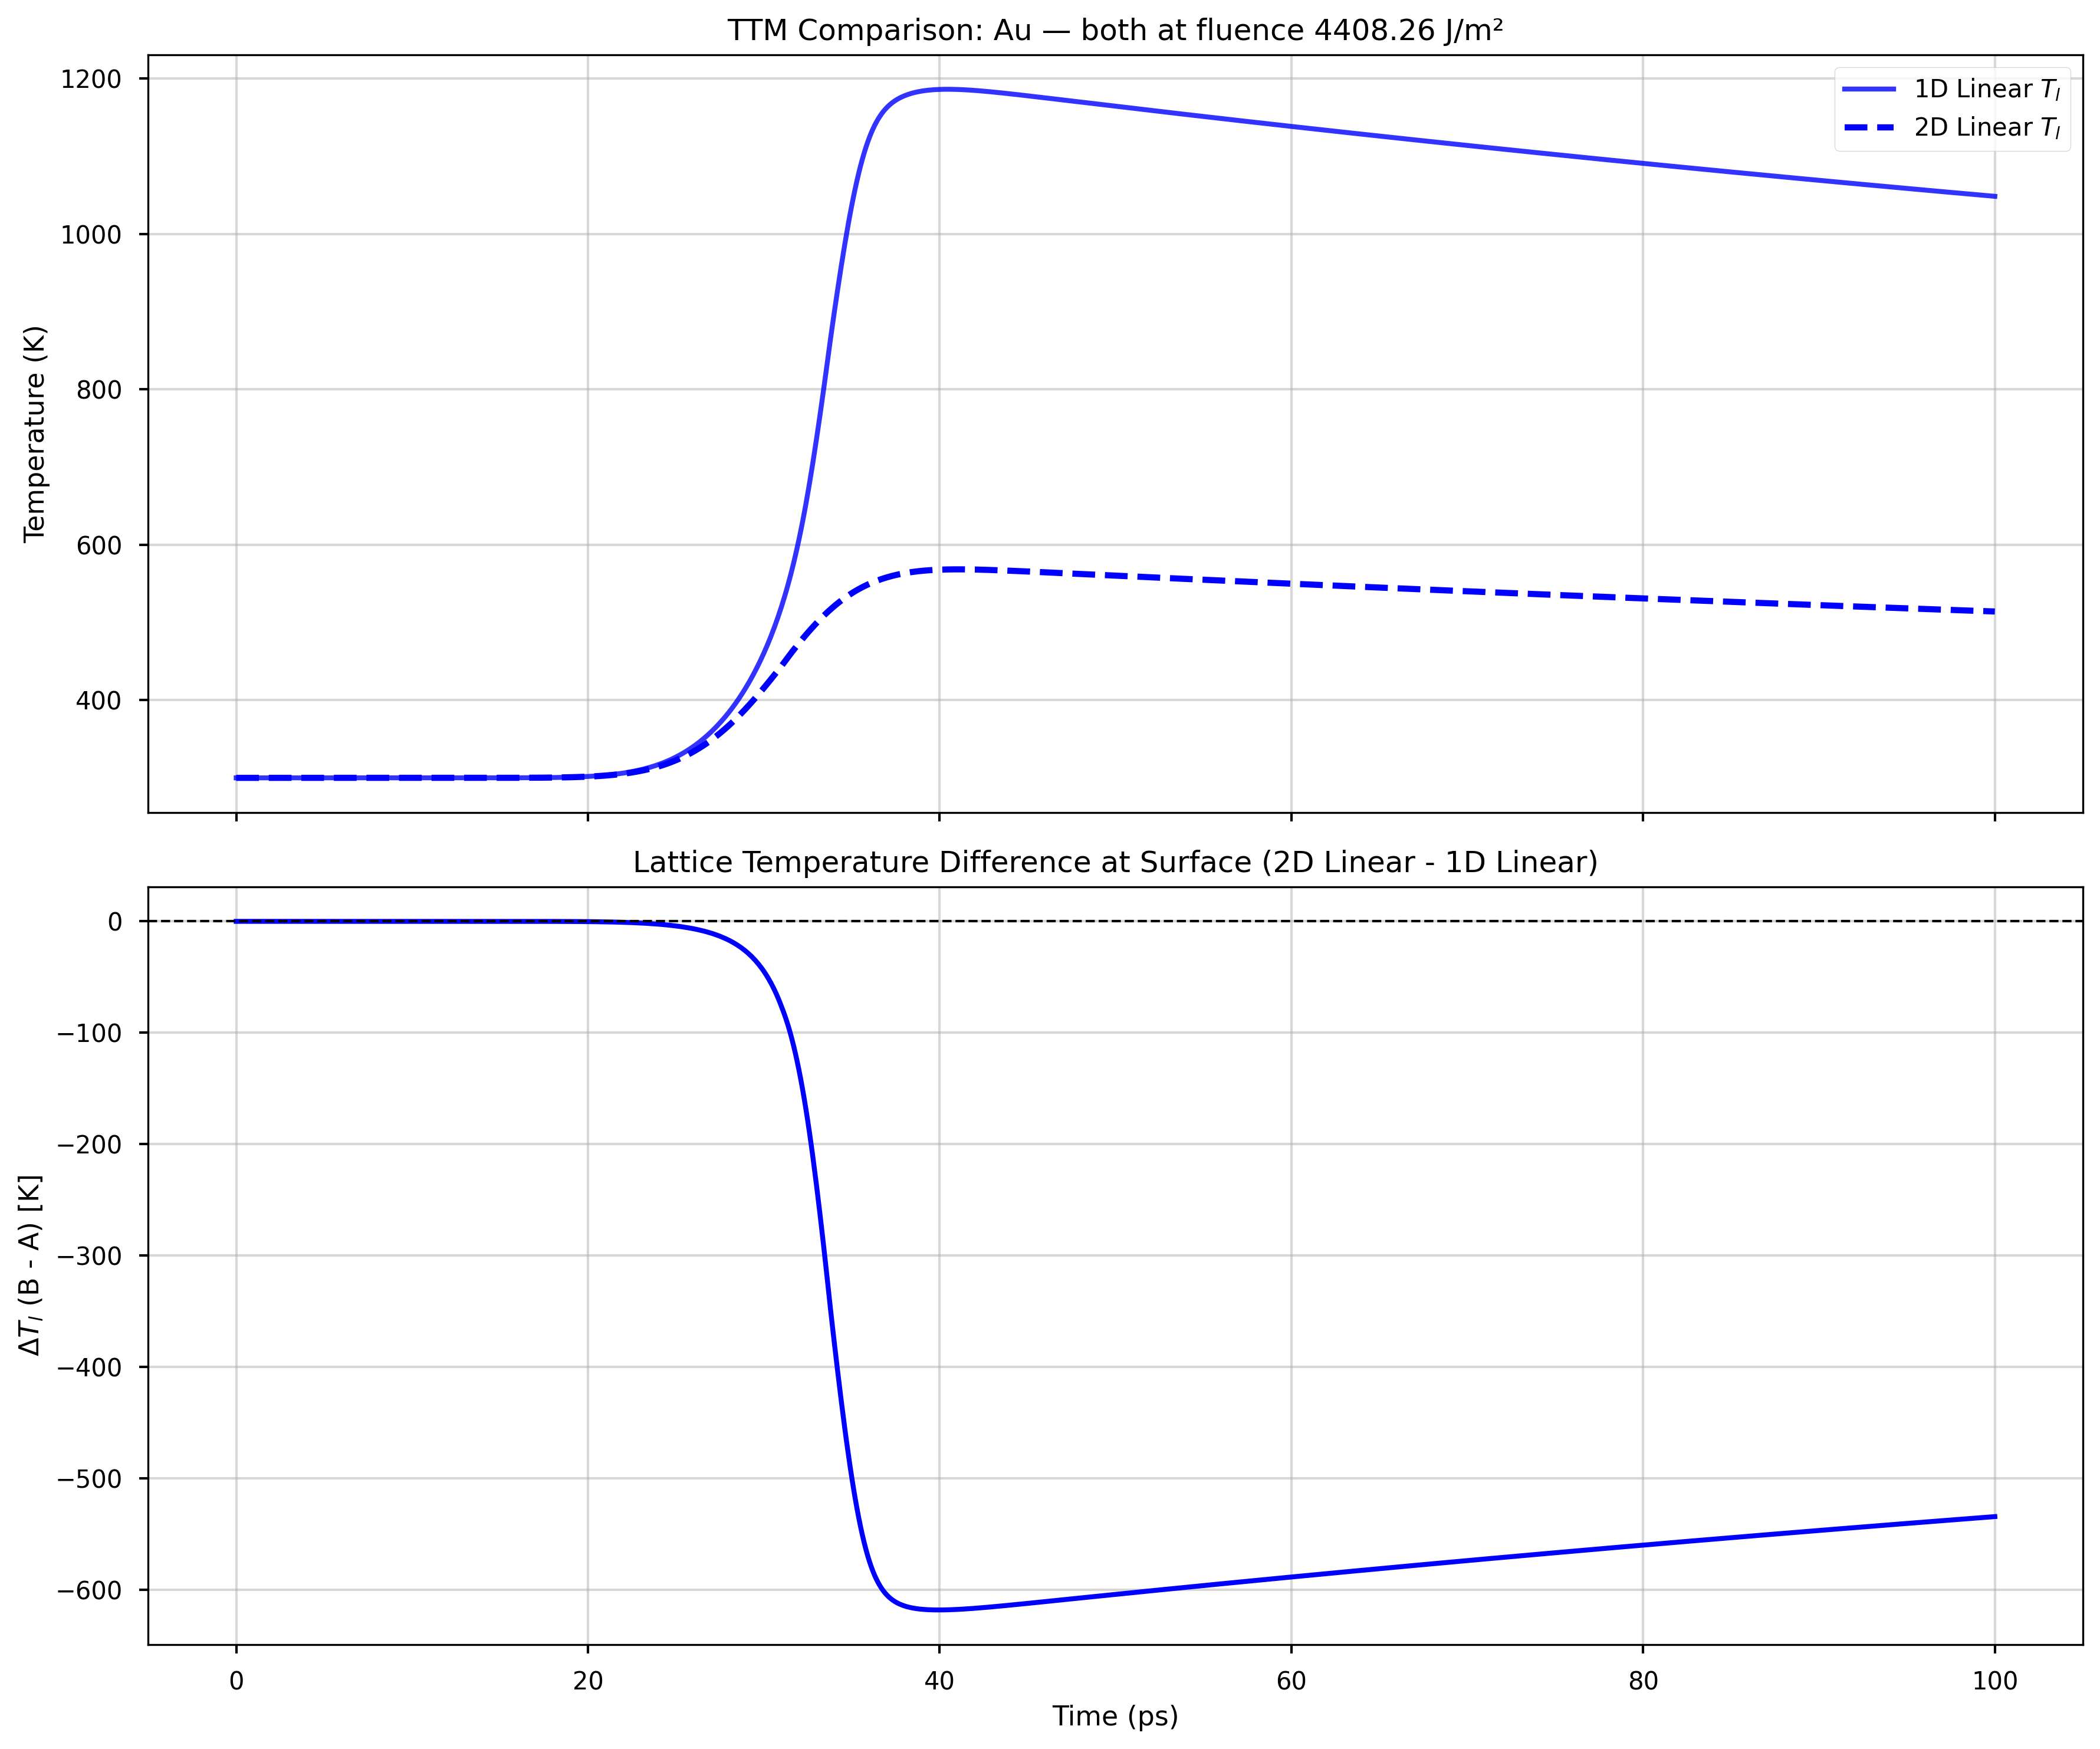
\includegraphics[width=0.32\linewidth]{figures/ch3/comparison_Au_linear.png}
    }\hfill
    \subfloat[Ni.\label{fig:ch3-comparison-linear-ni}]{%
        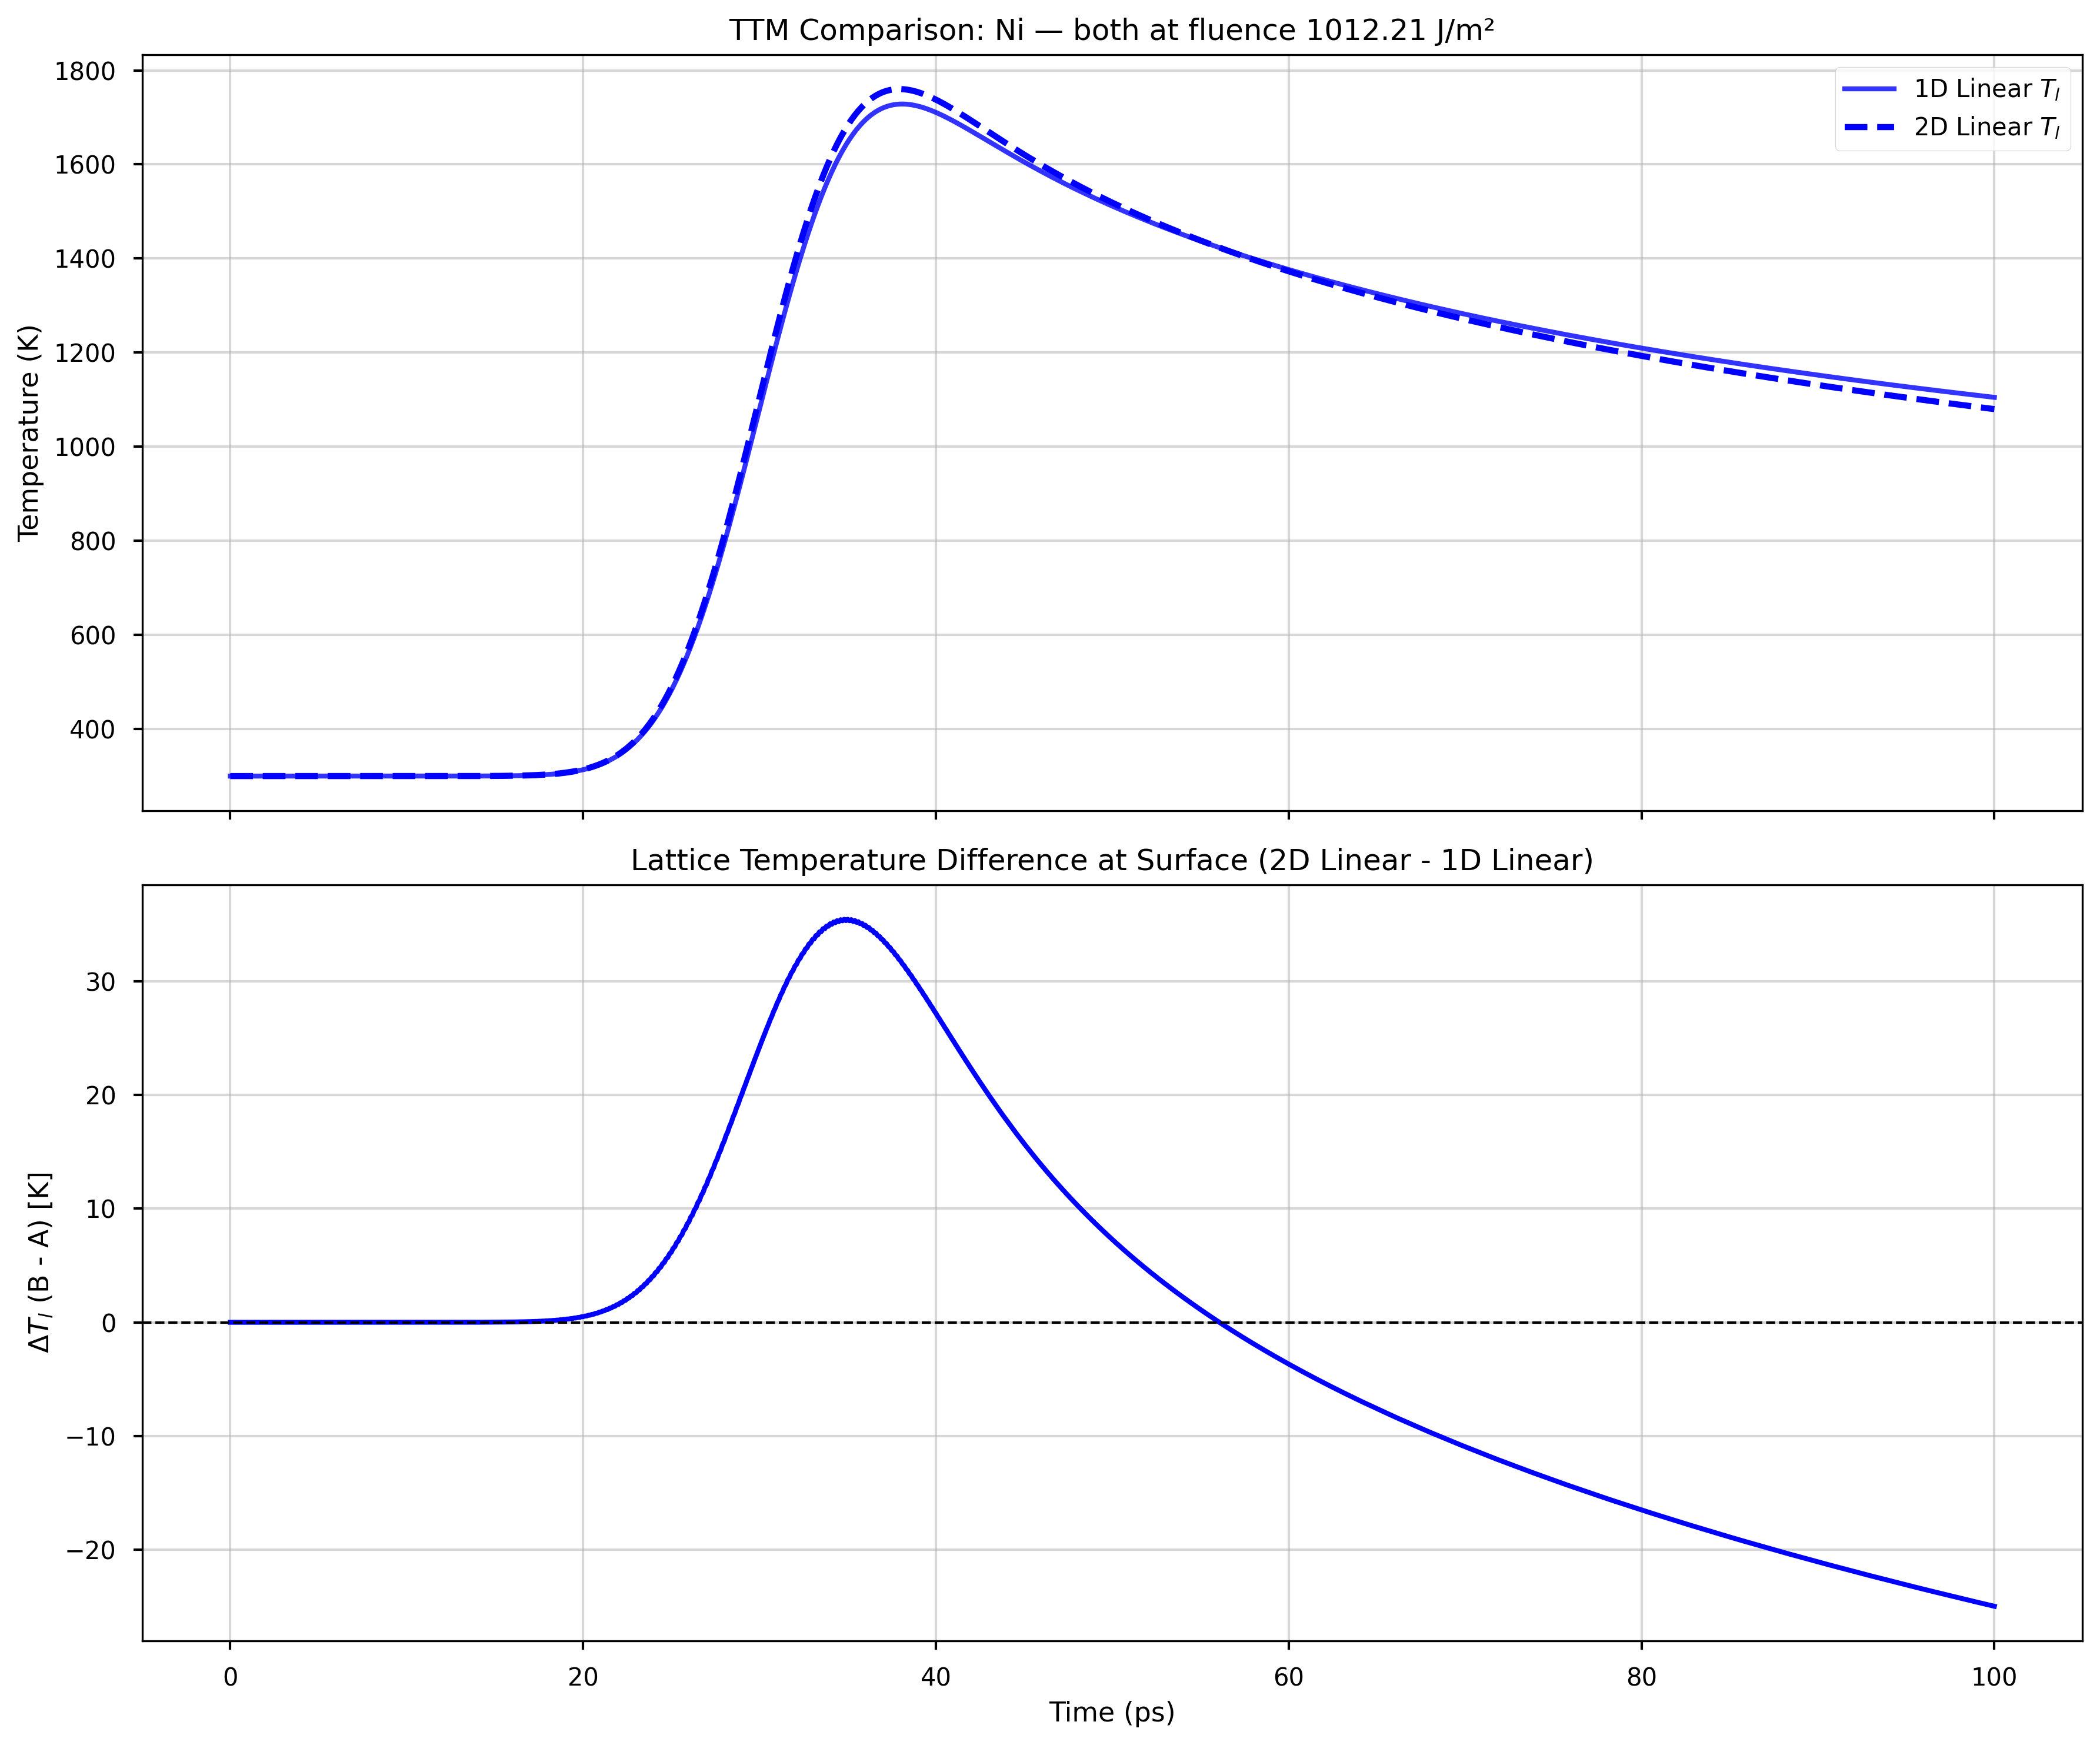
\includegraphics[width=0.32\linewidth]{figures/ch3/comparison_Ni_linear.png}
    }\hfill
    \subfloat[Cu.\label{fig:ch3-comparison-linear-cu}]{%
        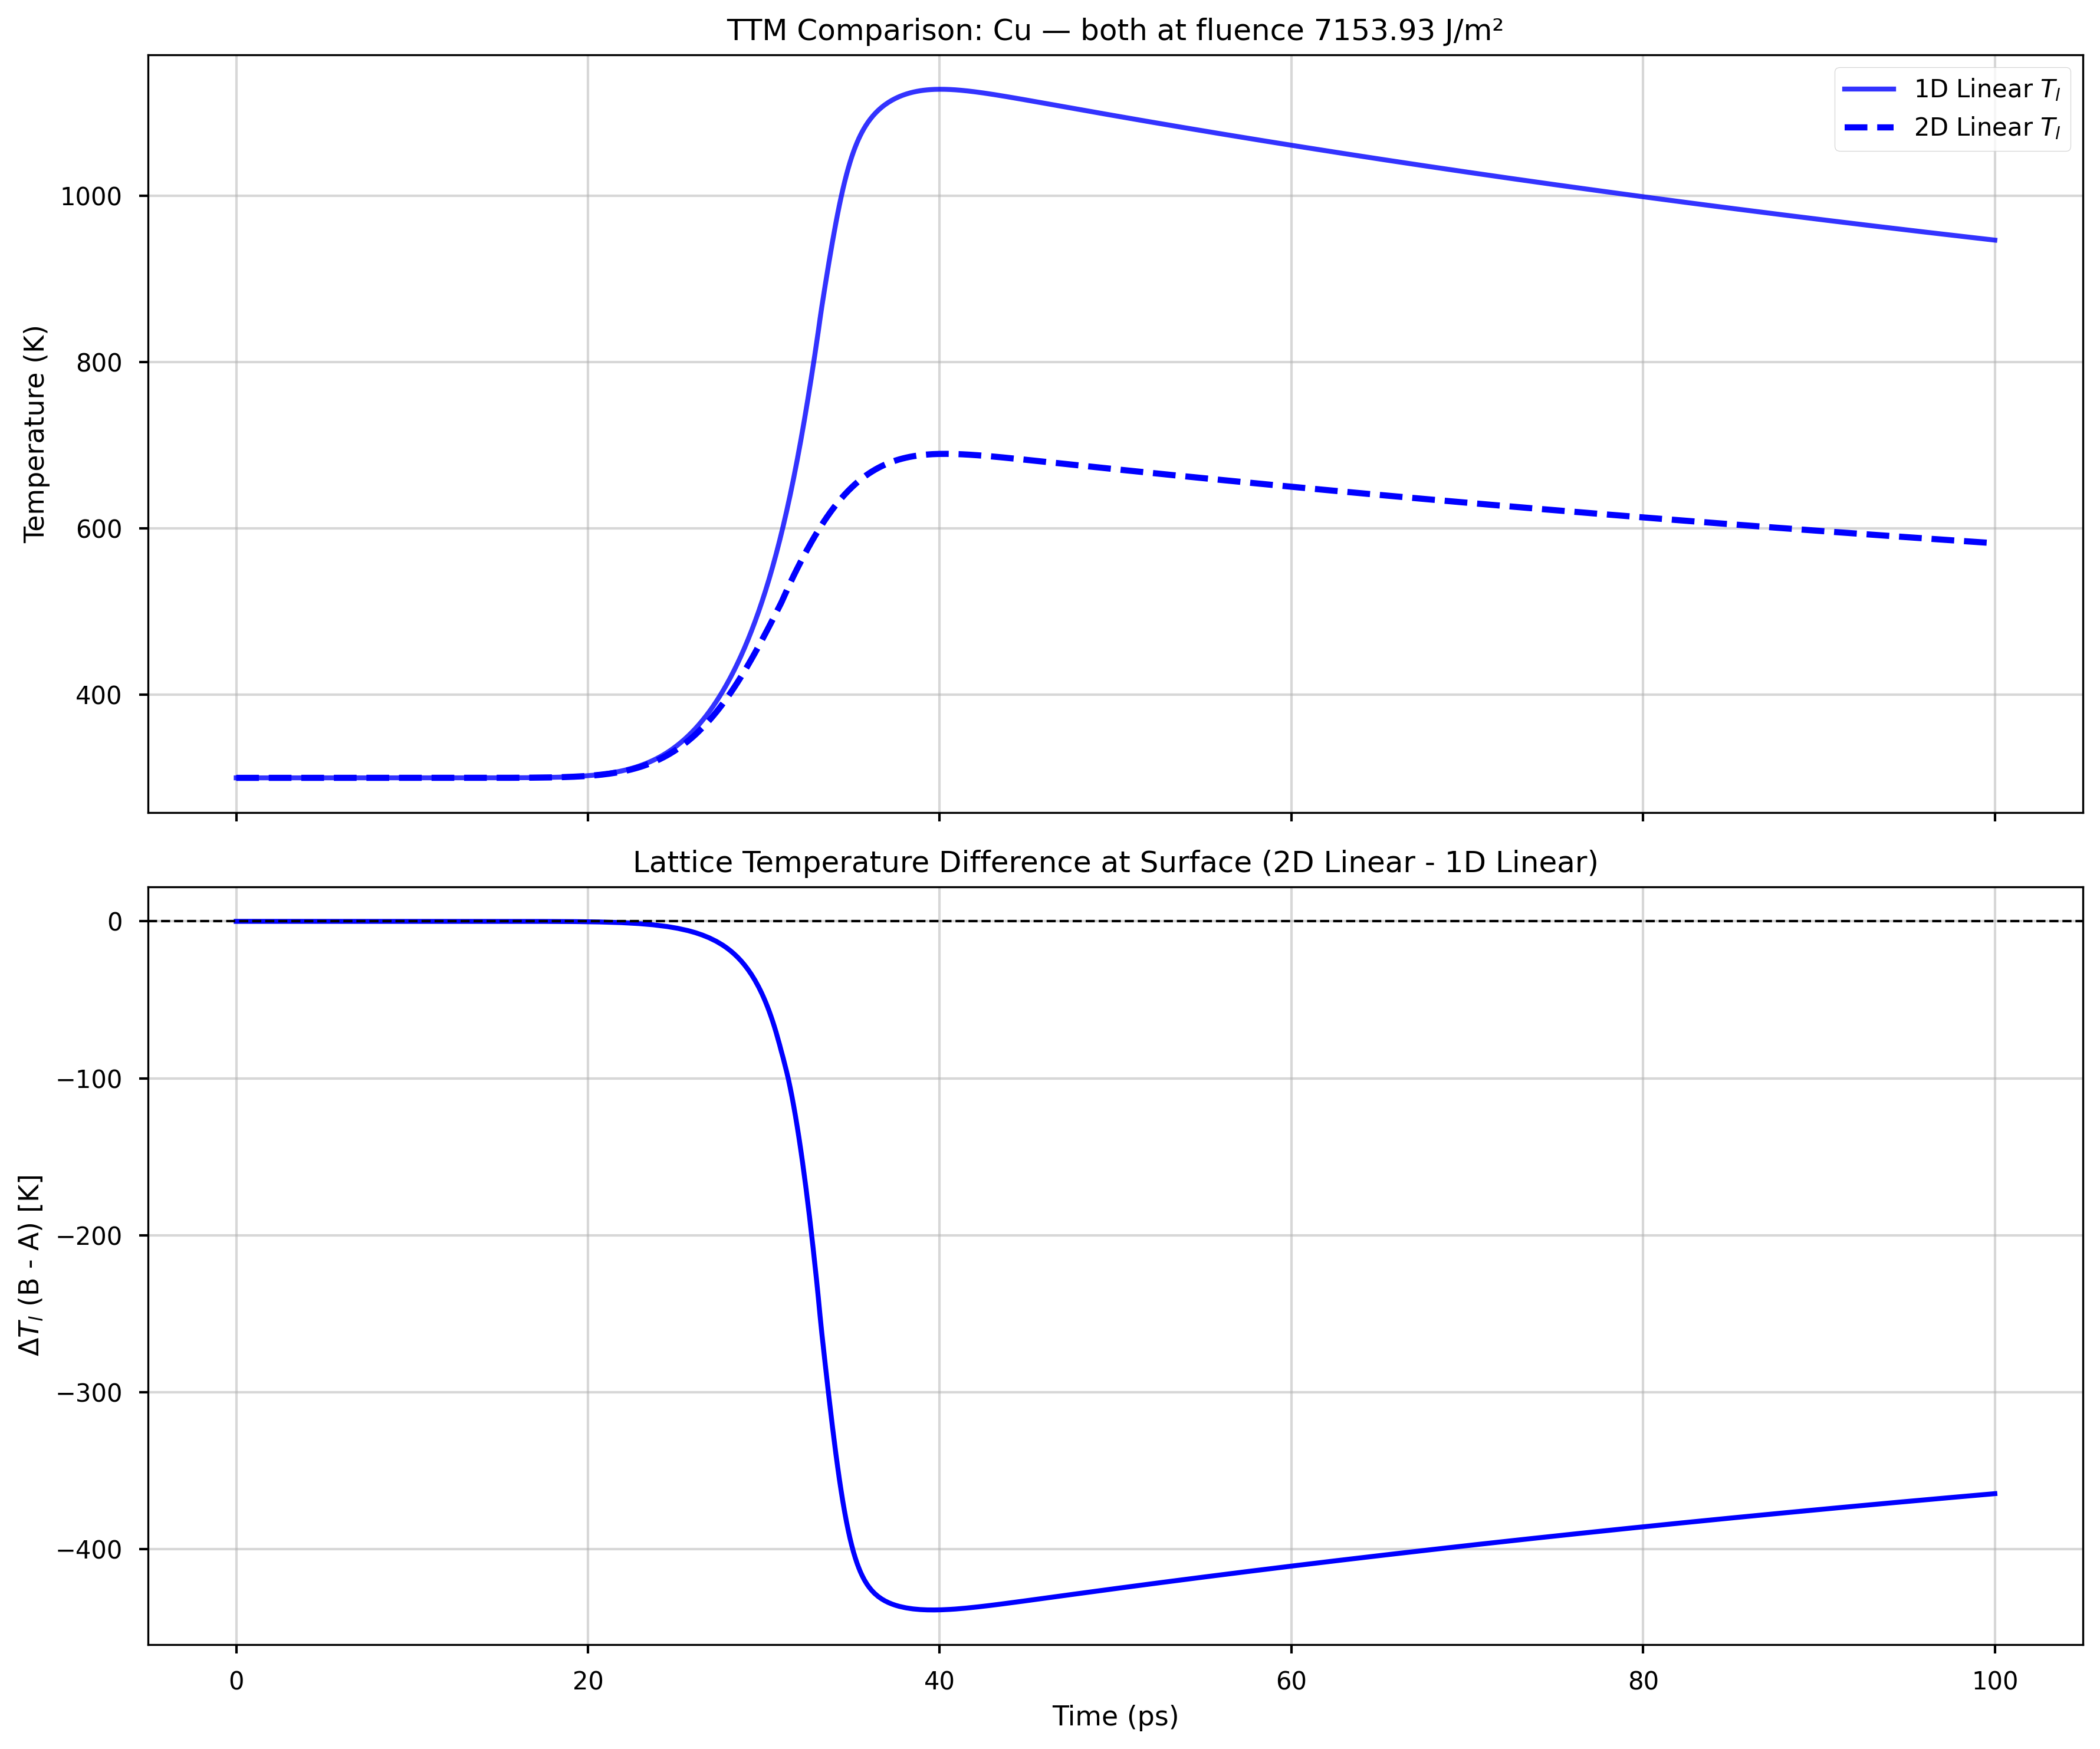
\includegraphics[width=0.32\linewidth]{figures/ch3/comparison_Cu_linear.png}
    }
    \caption{Comparison of 1D and 2D \emph{linear} pTTM predictions at the common fluence \(\hat F_{\mathrm{th}}^{\mathrm{1D,lin}}\) for each material. In each subfigure, the upper panel shows the surface lattice-temperature history, where the 2D signal is reduced to \(\max_x T_l(x,z_s,t)\). The lower panel shows the difference \(\Delta T_l(t)=T_l^{\mathrm{2D}}-T_l^{\mathrm{1D}}\).}
    \label{fig:ch3-1d-2d-comparison-linear-metals}
\end{figure}

\begin{figure}[H]
    \centering
    \subfloat[Au.\label{fig:ch3-comparison-nonlinear-au}]{%
        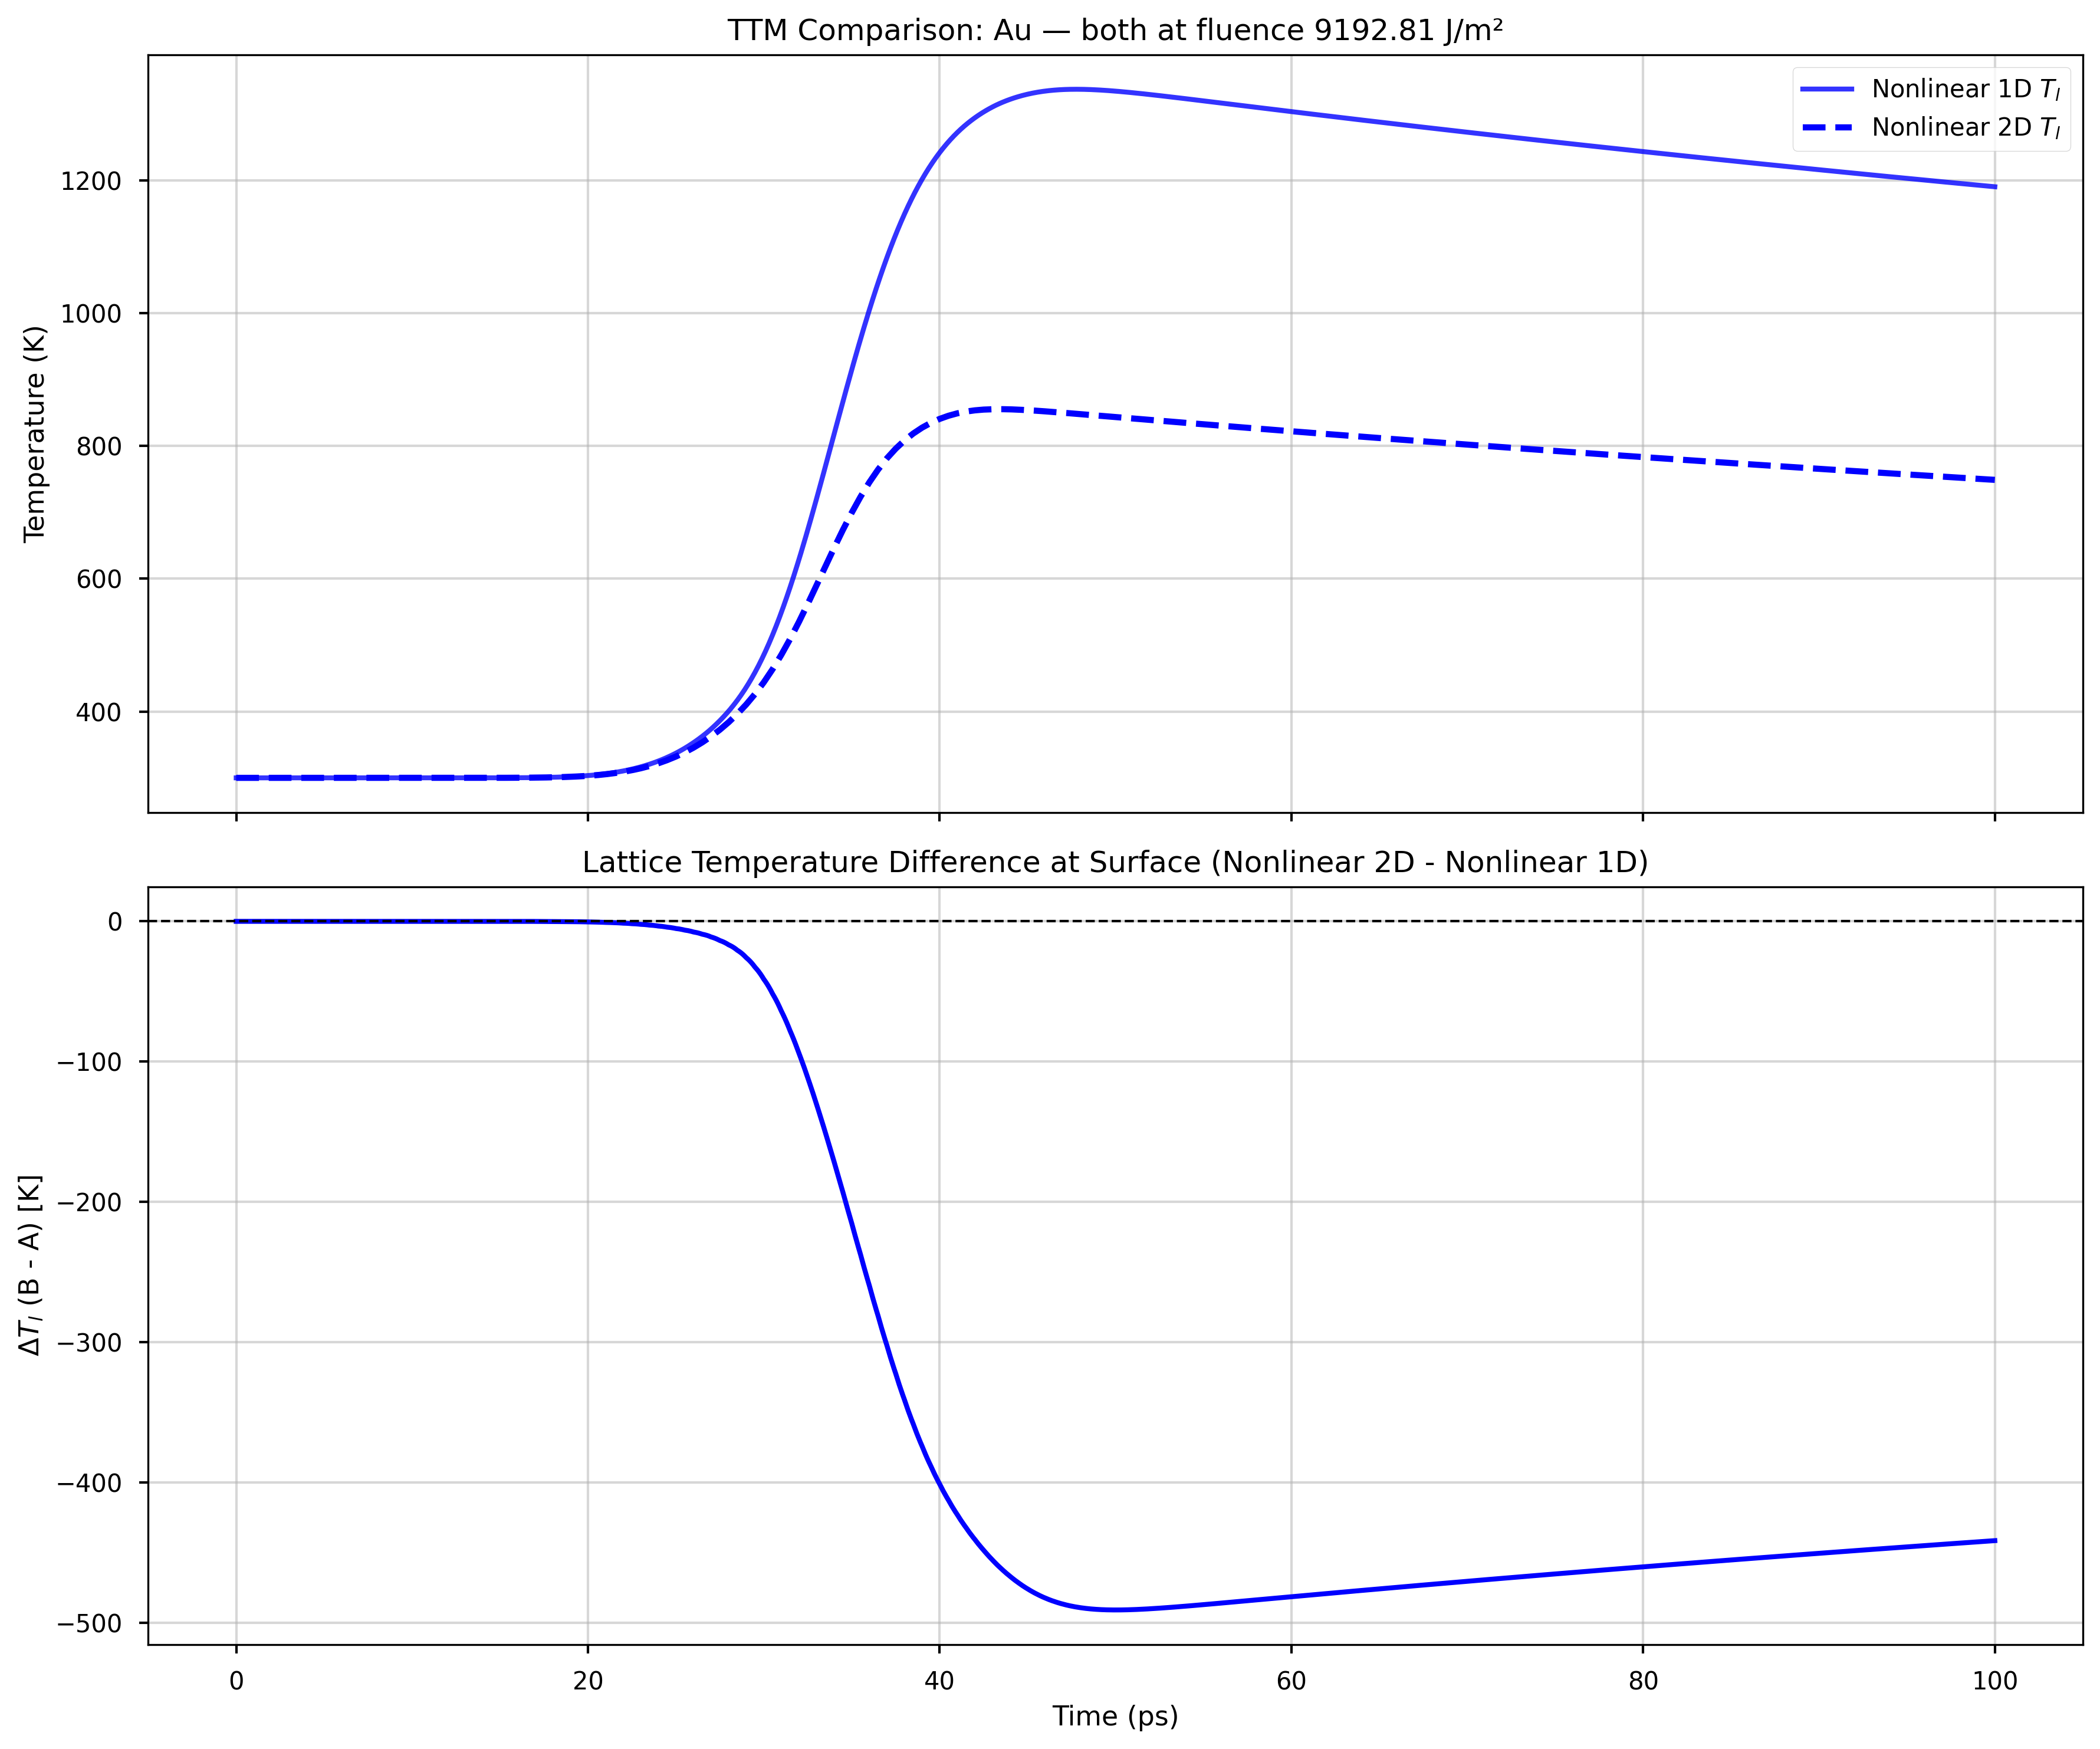
\includegraphics[width=0.32\linewidth]{figures/ch3/comparison_Au_nonlinear.png}
    }\hfill
    \subfloat[Ni.\label{fig:ch3-comparison-nonlinear-ni}]{%
        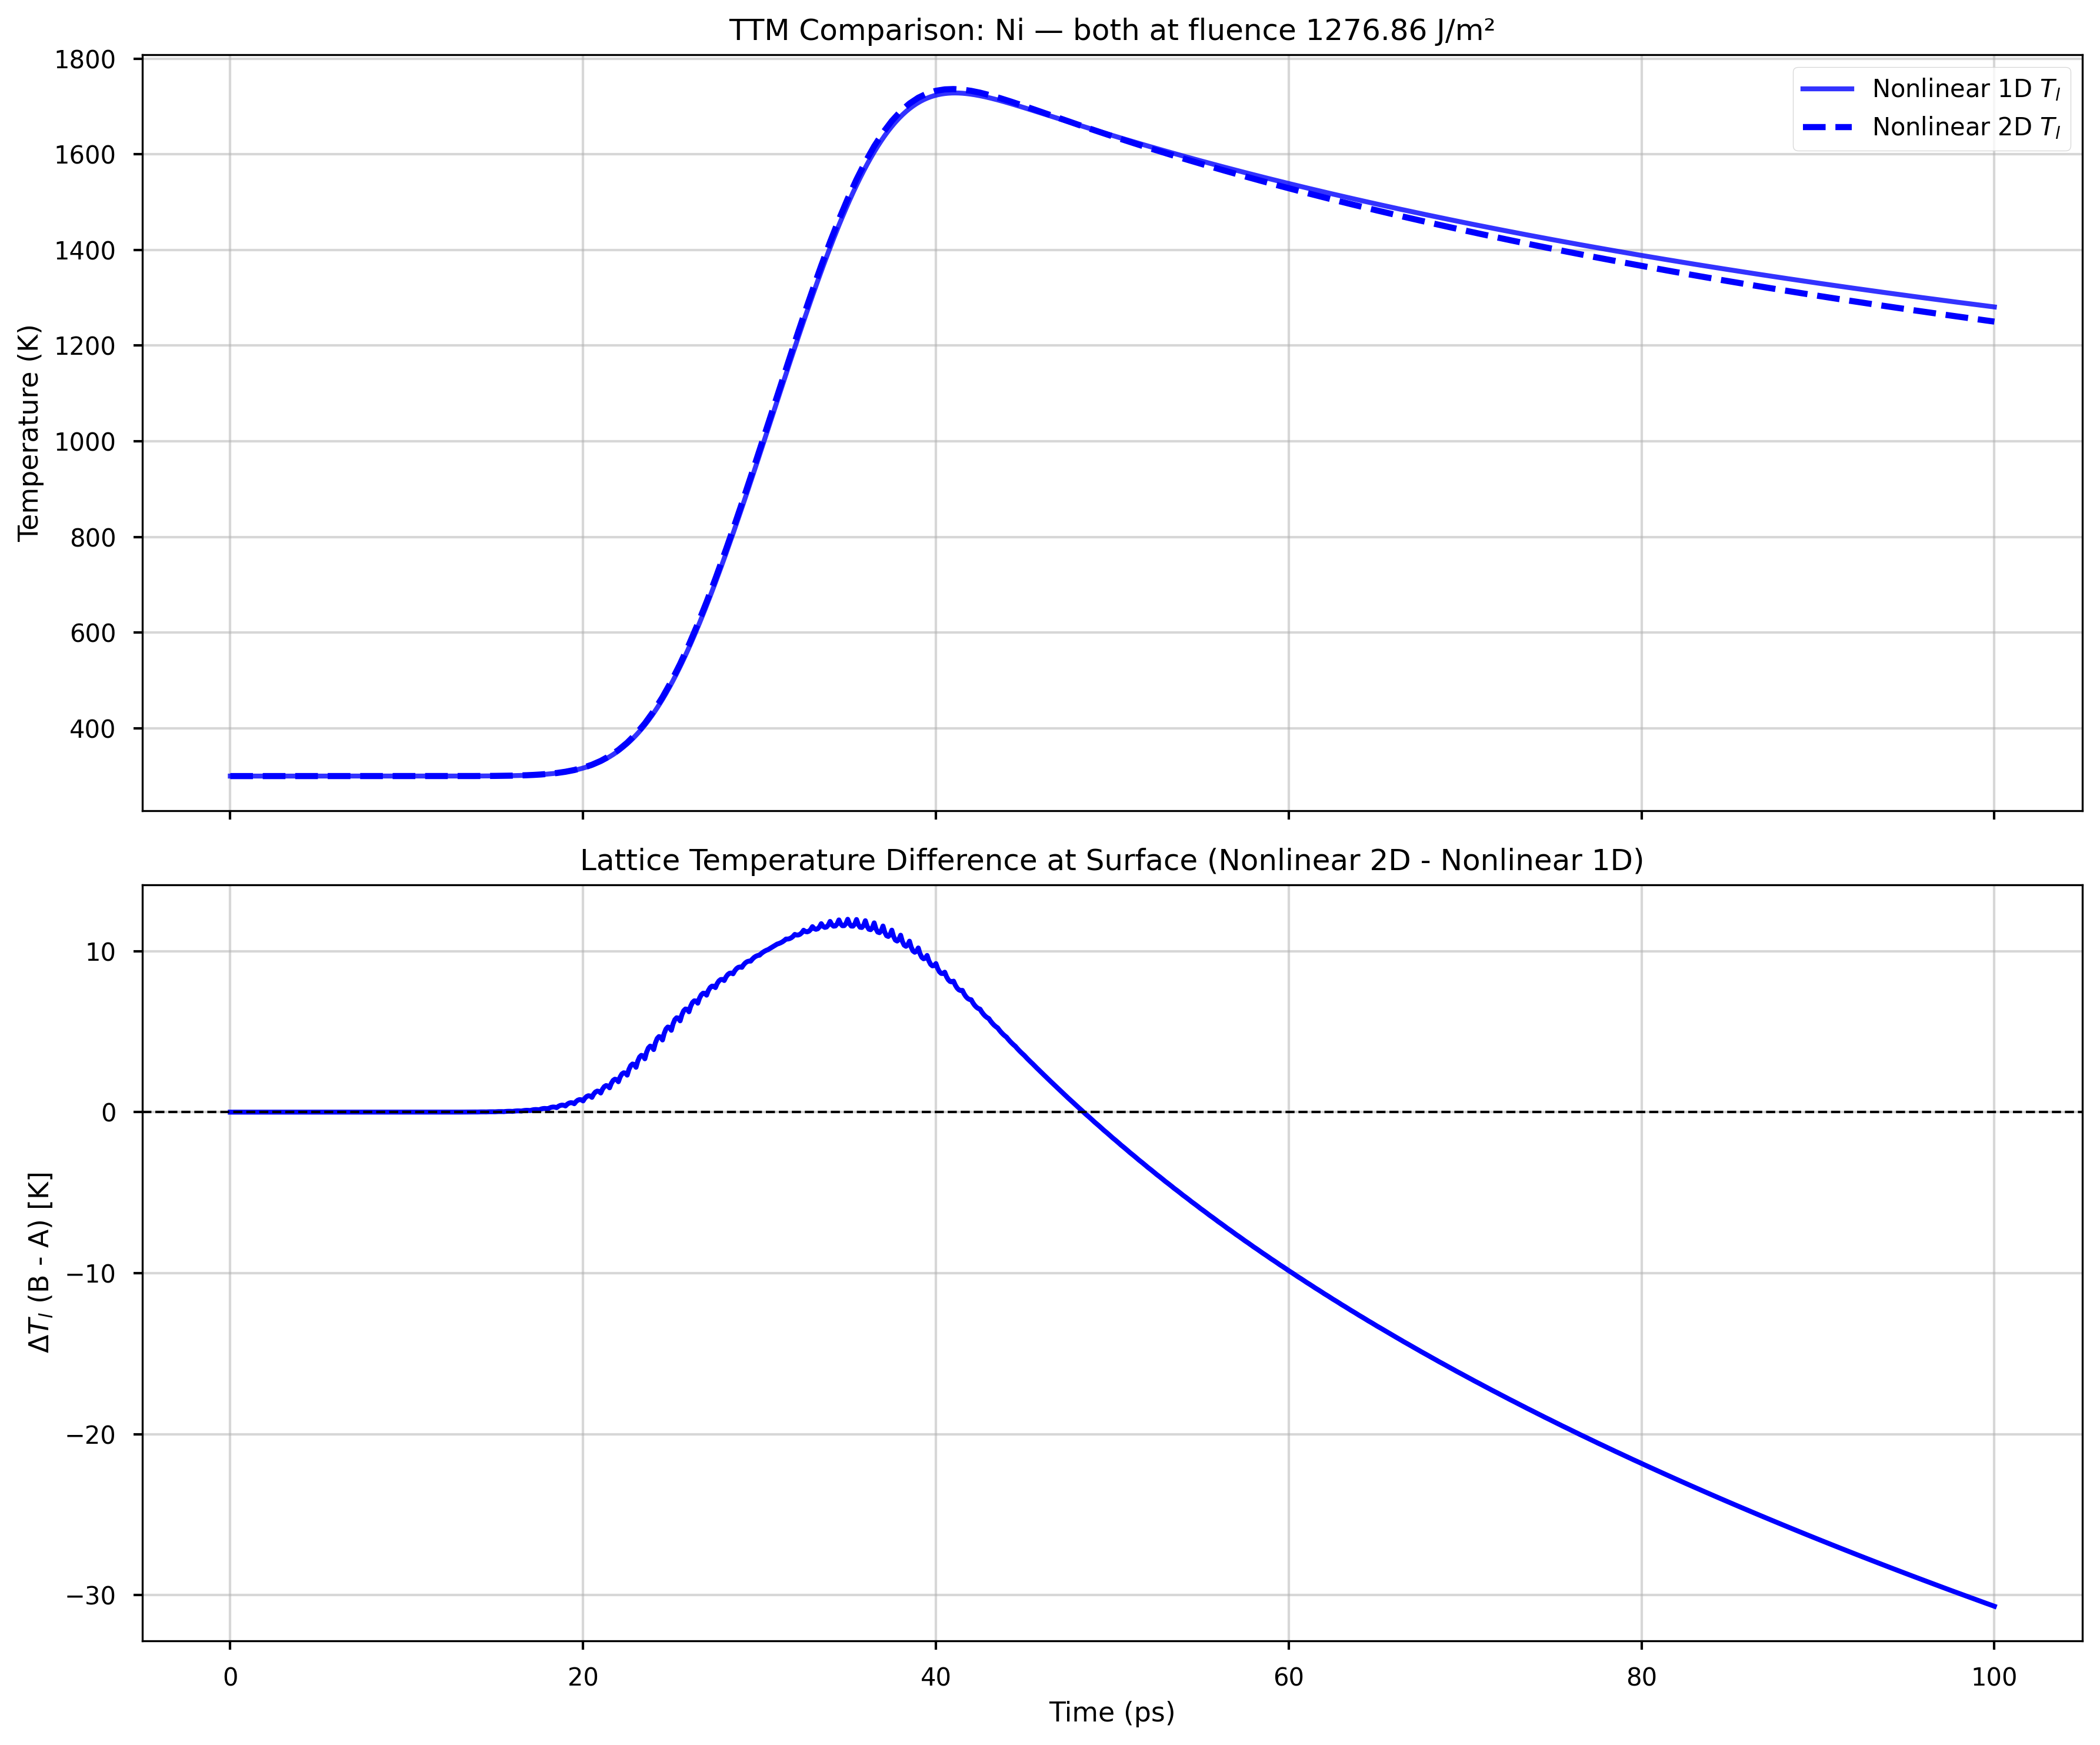
\includegraphics[width=0.32\linewidth]{figures/ch3/comparison_Ni_nonlinear.png}
    }\hfill
    \subfloat[Cu.\label{fig:ch3-comparison-nonlinear-cu}]{%
        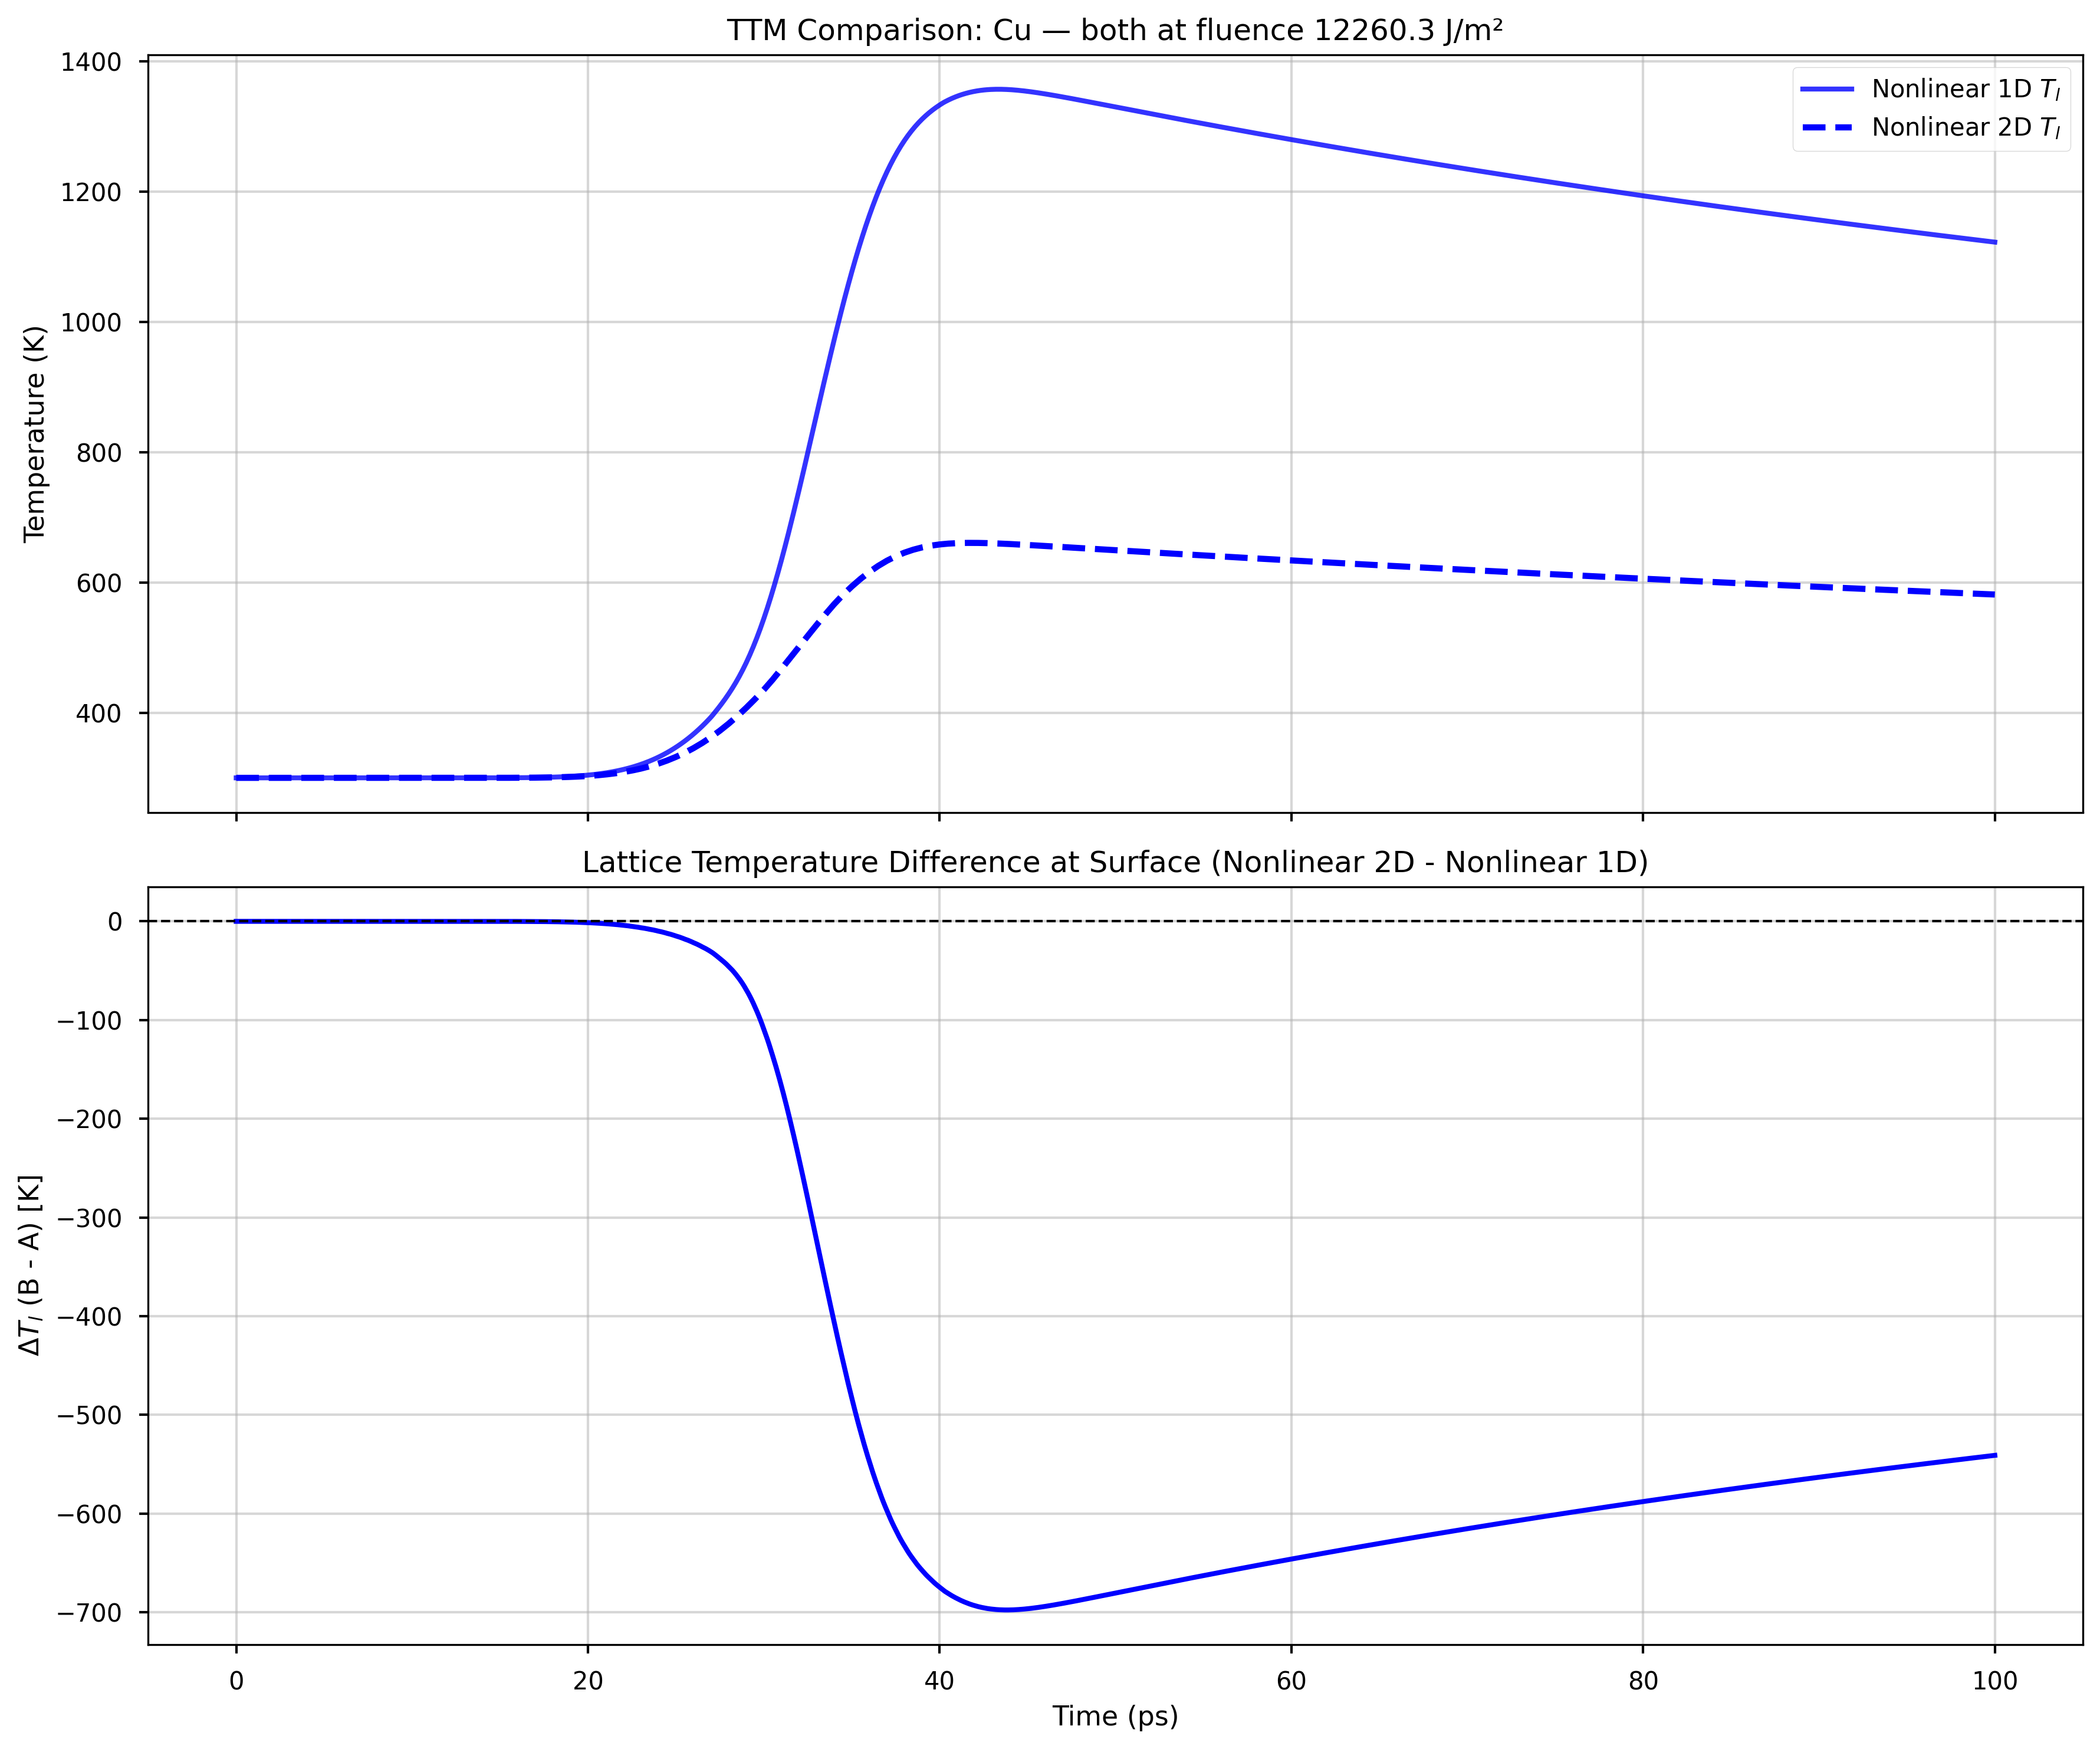
\includegraphics[width=0.32\linewidth]{figures/ch3/comparison_Cu_nonlinear.png}
    }
    \caption{Comparison of 1D and 2D \emph{nonlinear} pTTM predictions at the common fluence \(\hat F_{\mathrm{th}}^{\mathrm{1D,nl}}\) for each material. The upper panels show the representative surface lattice-temperature history, and the lower panels show \(\Delta T_l(t)=T_l^{\mathrm{2D}}-T_l^{\mathrm{1D}}\).}
    \label{fig:ch3-1d-2d-comparison-nonlinear-metals}
\end{figure}

\subsubsection{Linear versus nonlinear predictions at fixed dimensionality}
\label{sec:ch3-ablation-discussion-linvsnl}

Figures~\ref{fig:ch3-comparison-linear-vs-nonlinear-1d-metals} and
\ref{fig:ch3-comparison-linear-vs-nonlinear-2d-metals} compare the linear
and nonlinear models at the same fluence, chosen here as the linear-model
threshold in the corresponding dimension. In every case, the nonlinear
lattice temperature stays below the linear one during the relevant
heating interval. The lower panels show that the difference
\(\Delta T_l(t)=T_l^{\mathrm{nl}}-T_l^{\mathrm{lin}}\) is negative by
hundreds of kelvin near the peak for Au, Ni, and Cu in both 1D and 2D.
This directly explains why the nonlinear threshold is systematically
higher than the linear one.

Quantitatively, the nonlinear threshold exceeds the linear threshold by
about \(108.5\%\) for Au, \(26.1\%\) for Ni, and \(71.4\%\) for Cu in 1D.
In 2D the corresponding increases are about \(93.8\%\) for Au,
\(28.1\%\) for Ni, and \(59.4\%\) for Cu. These differences are several
orders of magnitude larger than the bisection half-width
\(\delta F_{\mathrm{bis}}\), so the dominant uncertainty in the threshold
prediction is not the search algorithm but the underlying constitutive
model.

\begin{figure}[H]
    \centering
    \subfloat[Au.\label{fig:ch3-comparison-linear-vs-nonlinear-1d-au}]{%
        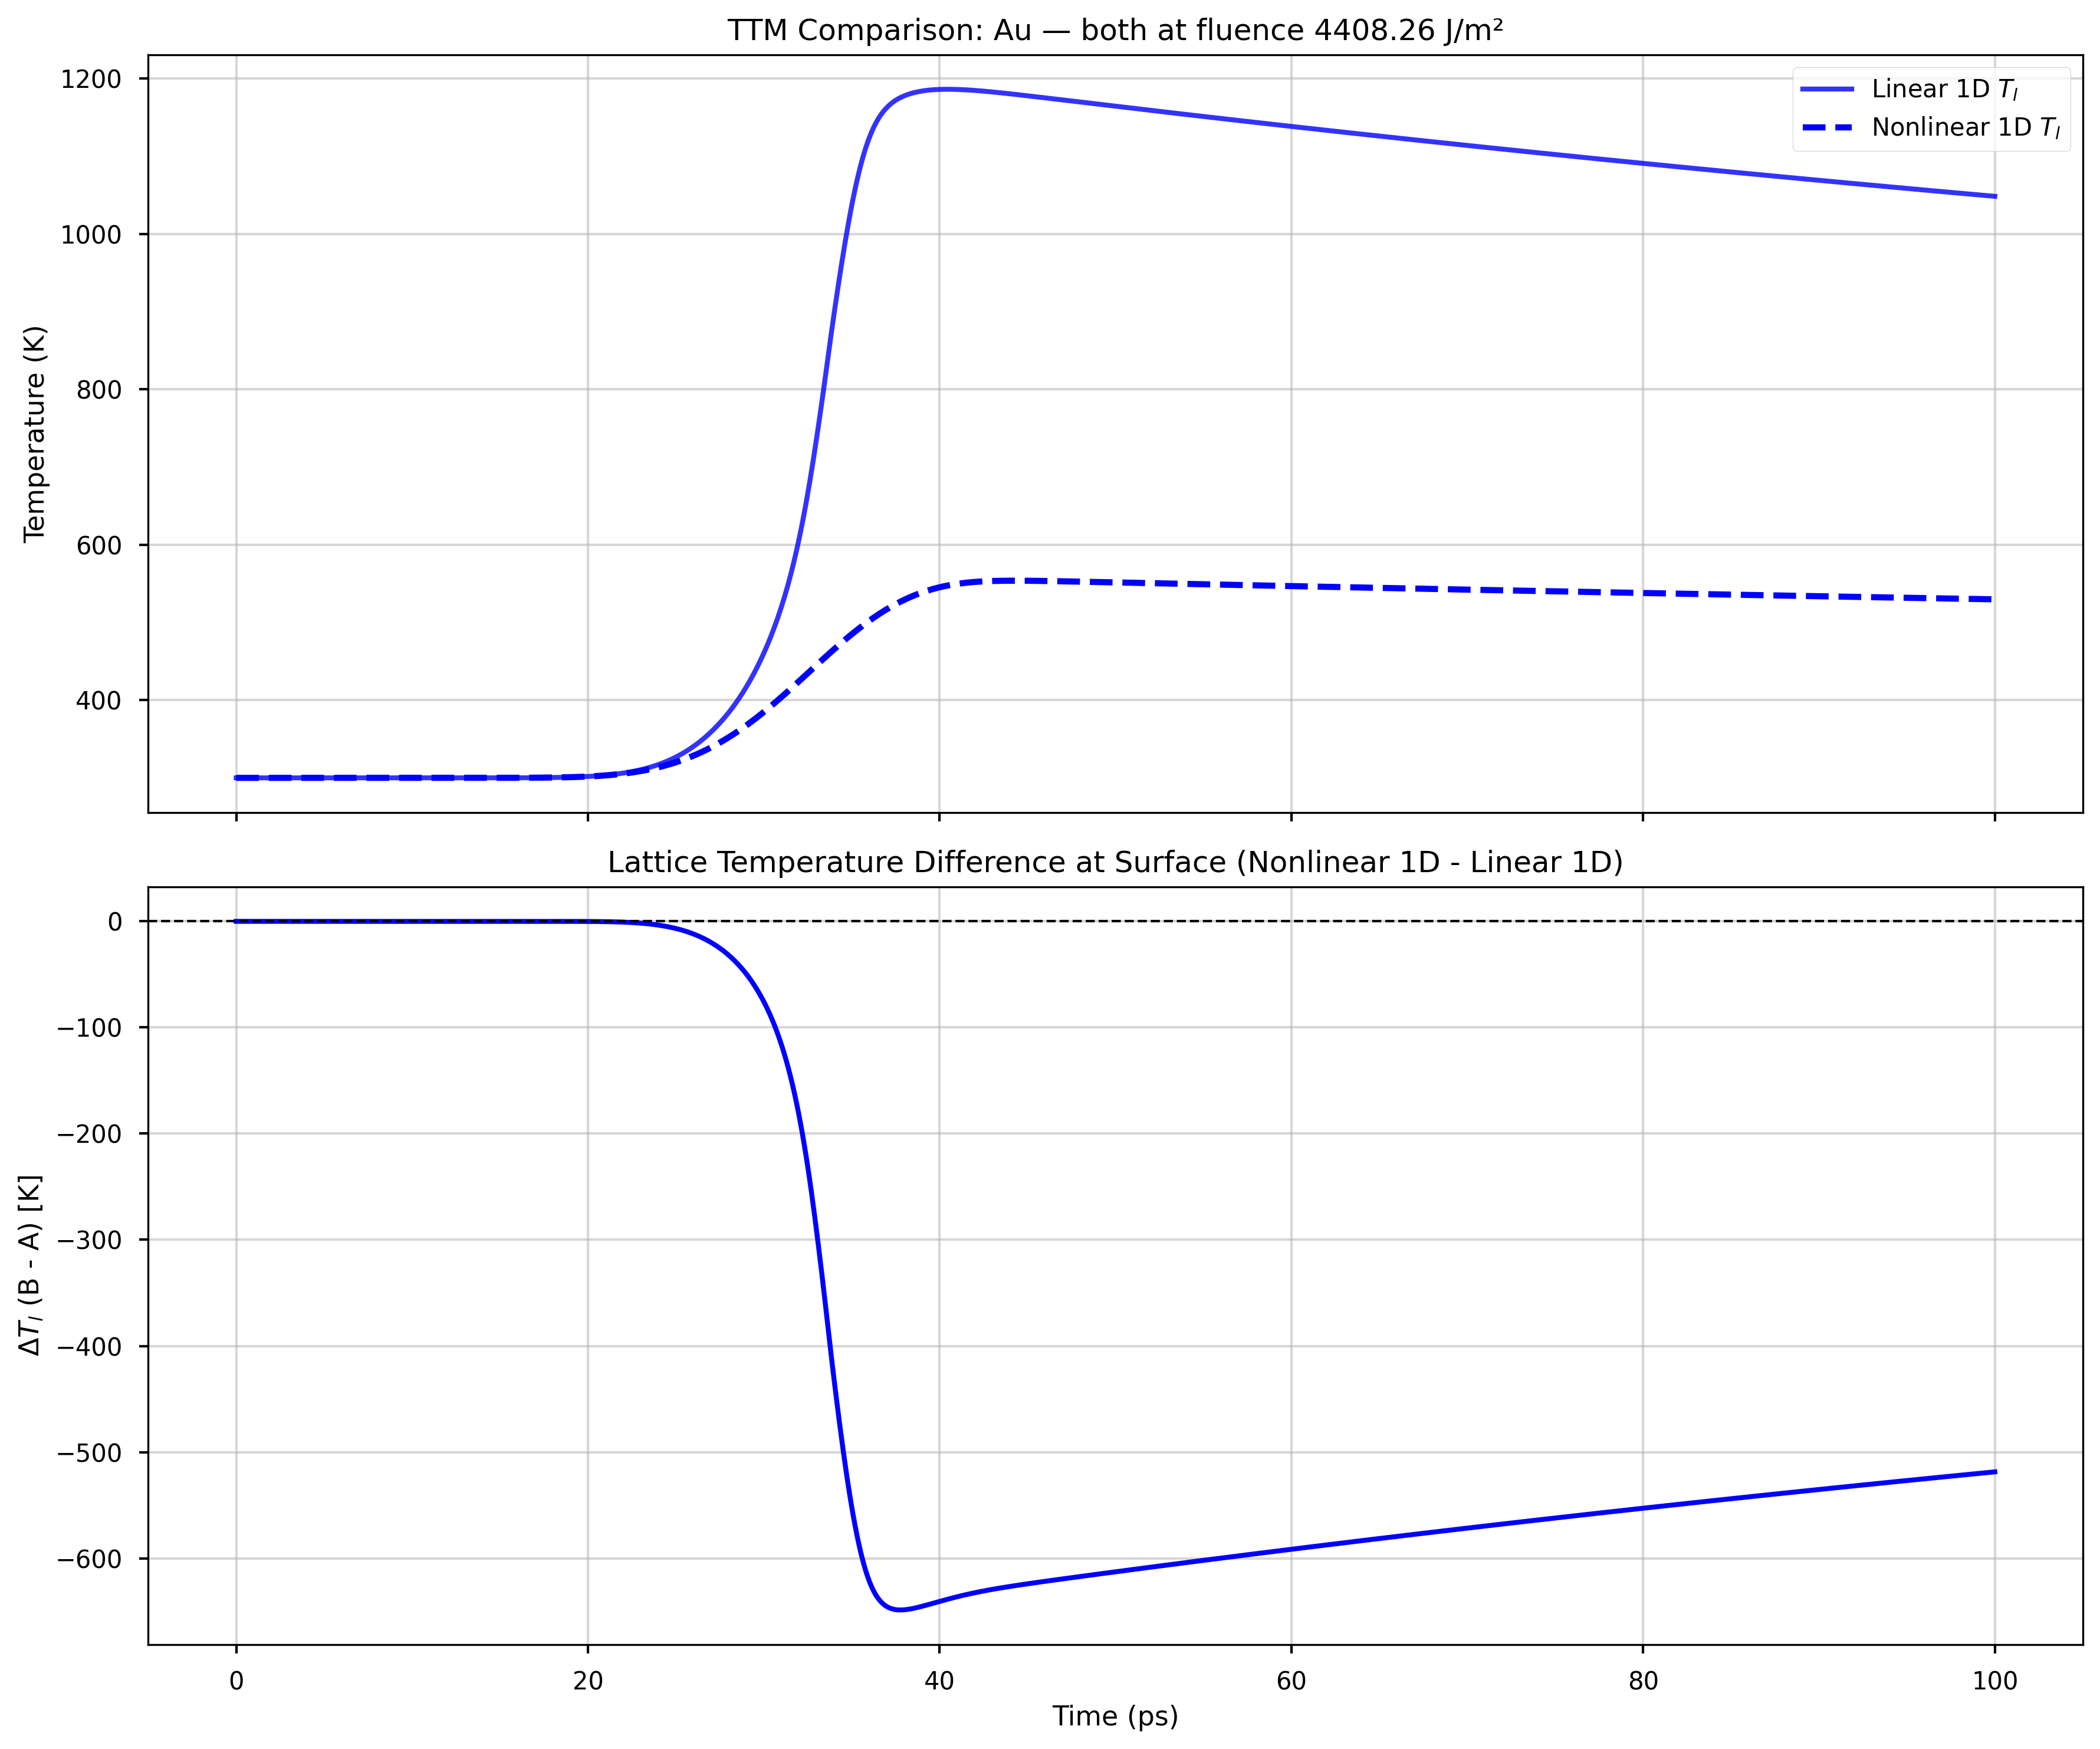
\includegraphics[width=0.32\linewidth]{figures/ch3/comparison_Au_linear_vs_nonlinear_1d.png}
    }\hfill
    \subfloat[Ni.\label{fig:ch3-comparison-linear-vs-nonlinear-1d-ni}]{%
        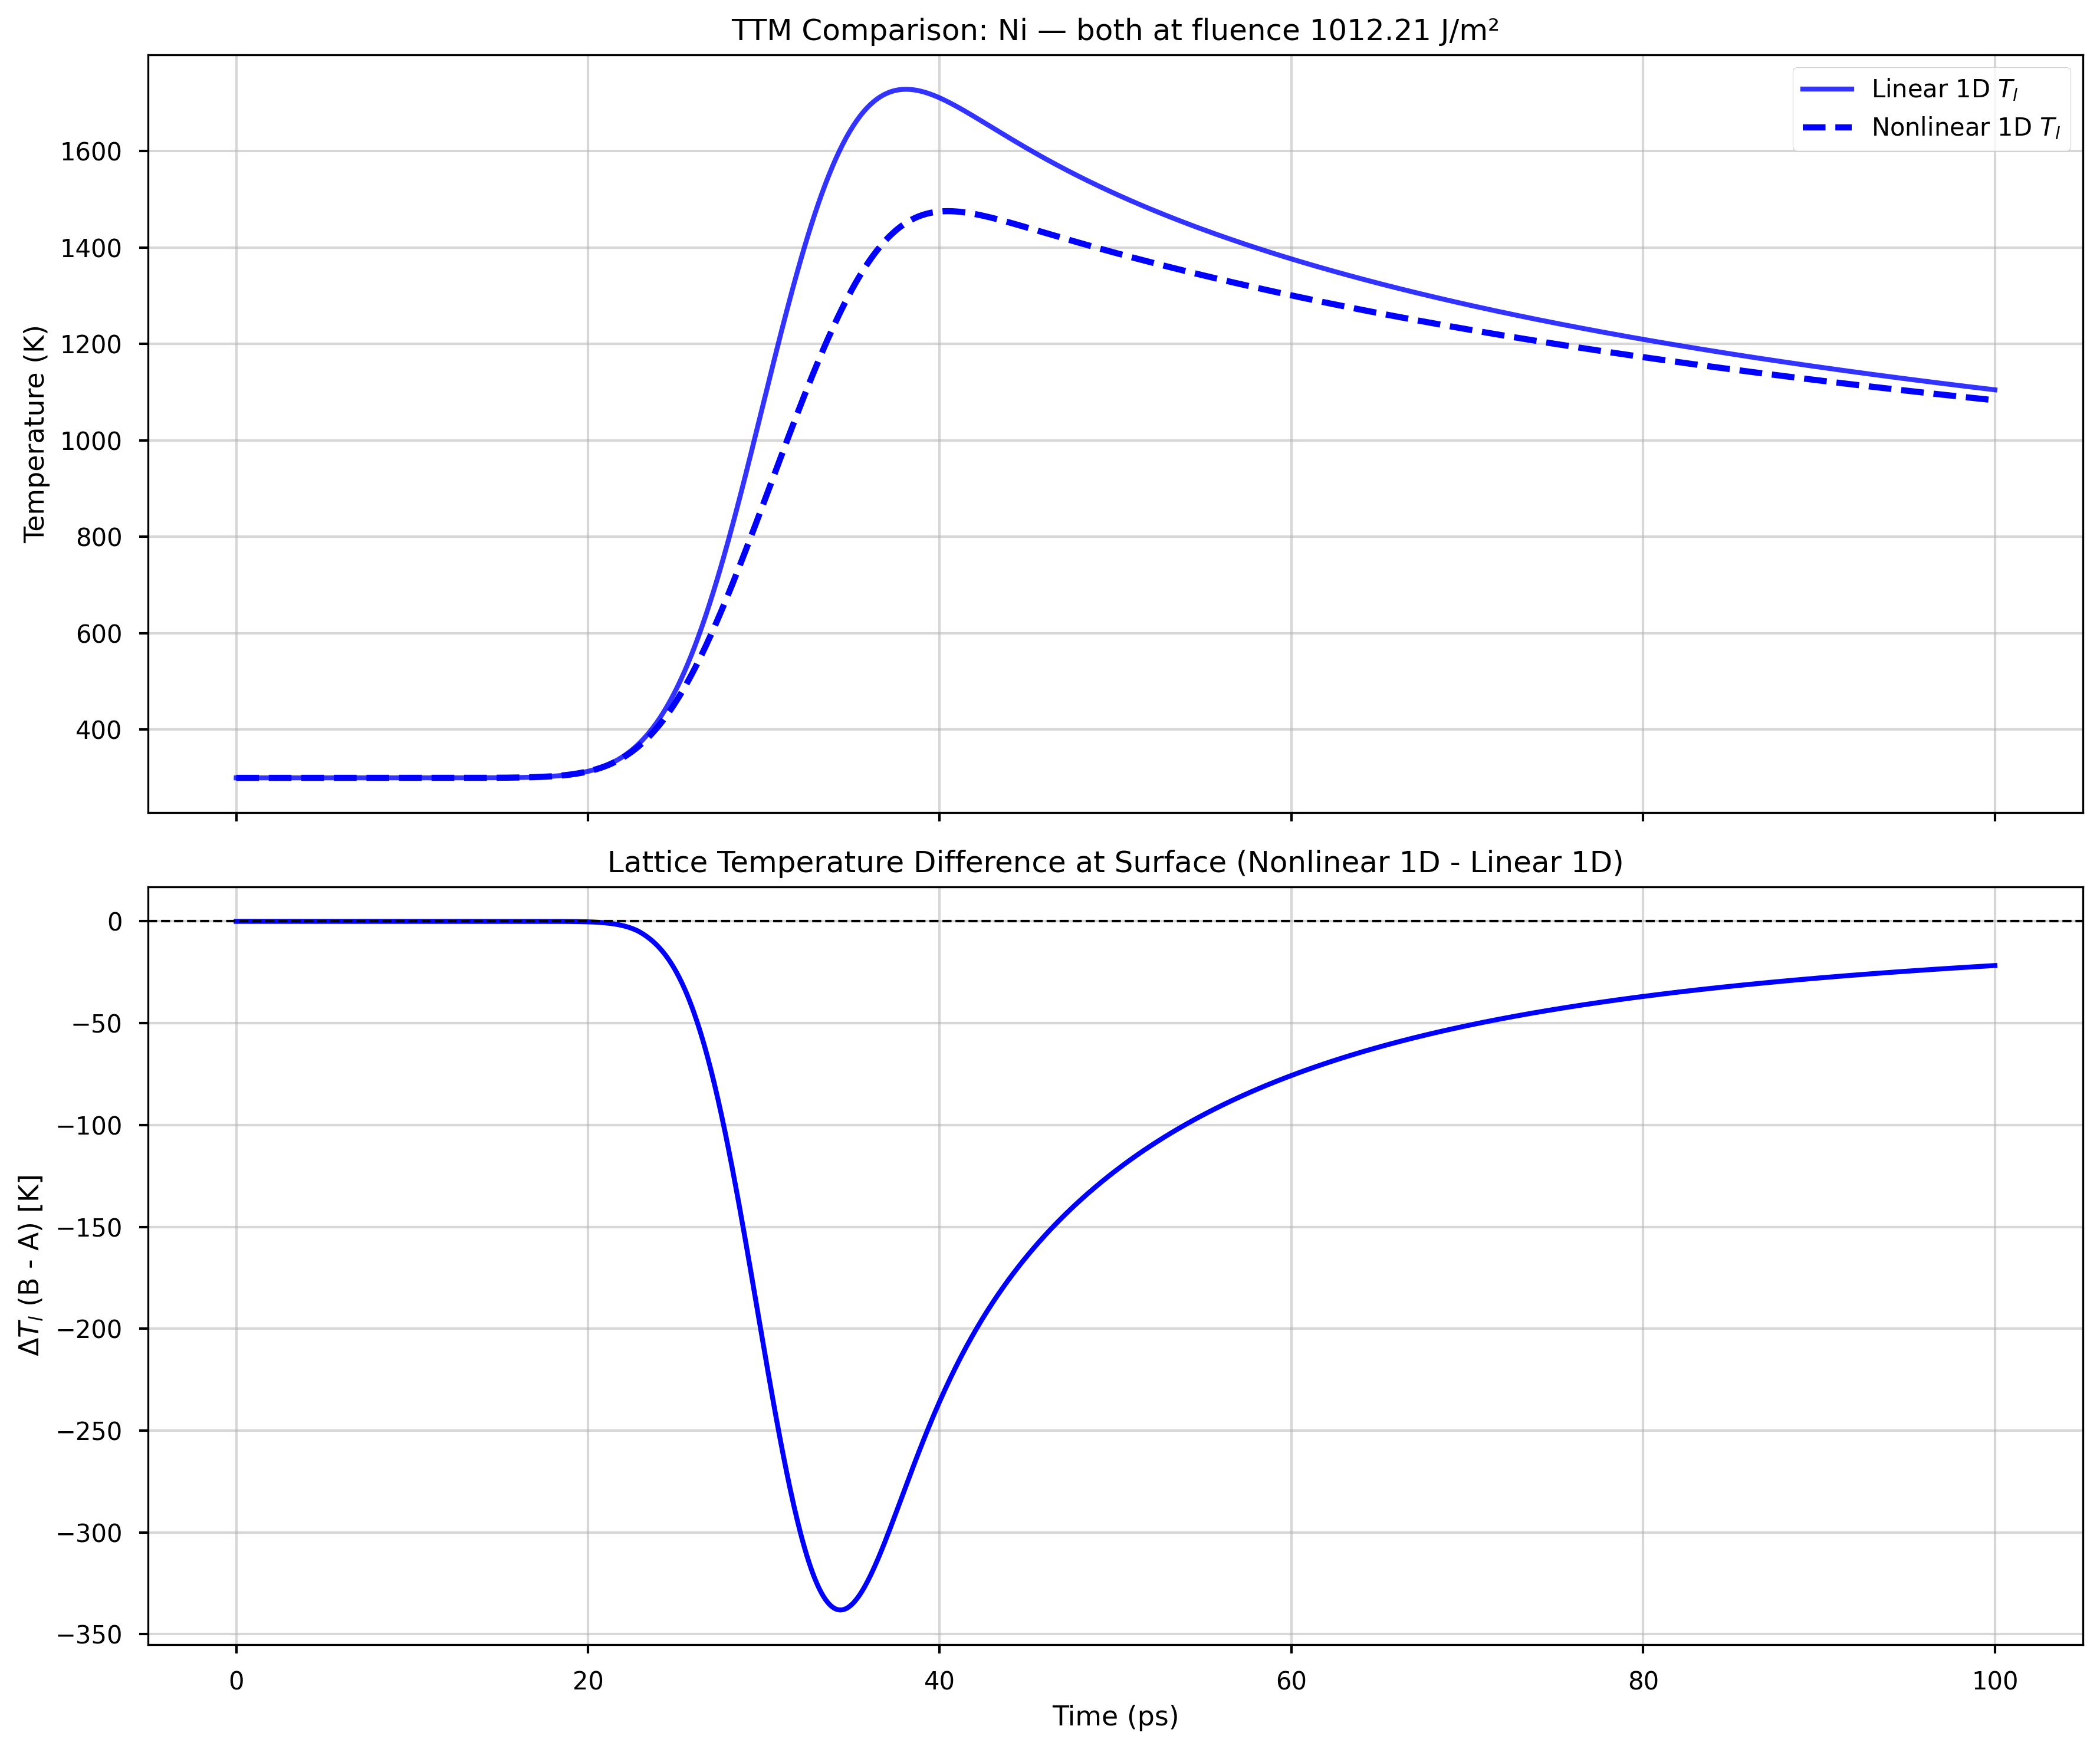
\includegraphics[width=0.32\linewidth]{figures/ch3/comparison_Ni_linear_vs_nonlinear_1d.png}
    }\hfill
    \subfloat[Cu.\label{fig:ch3-comparison-linear-vs-nonlinear-1d-cu}]{%
        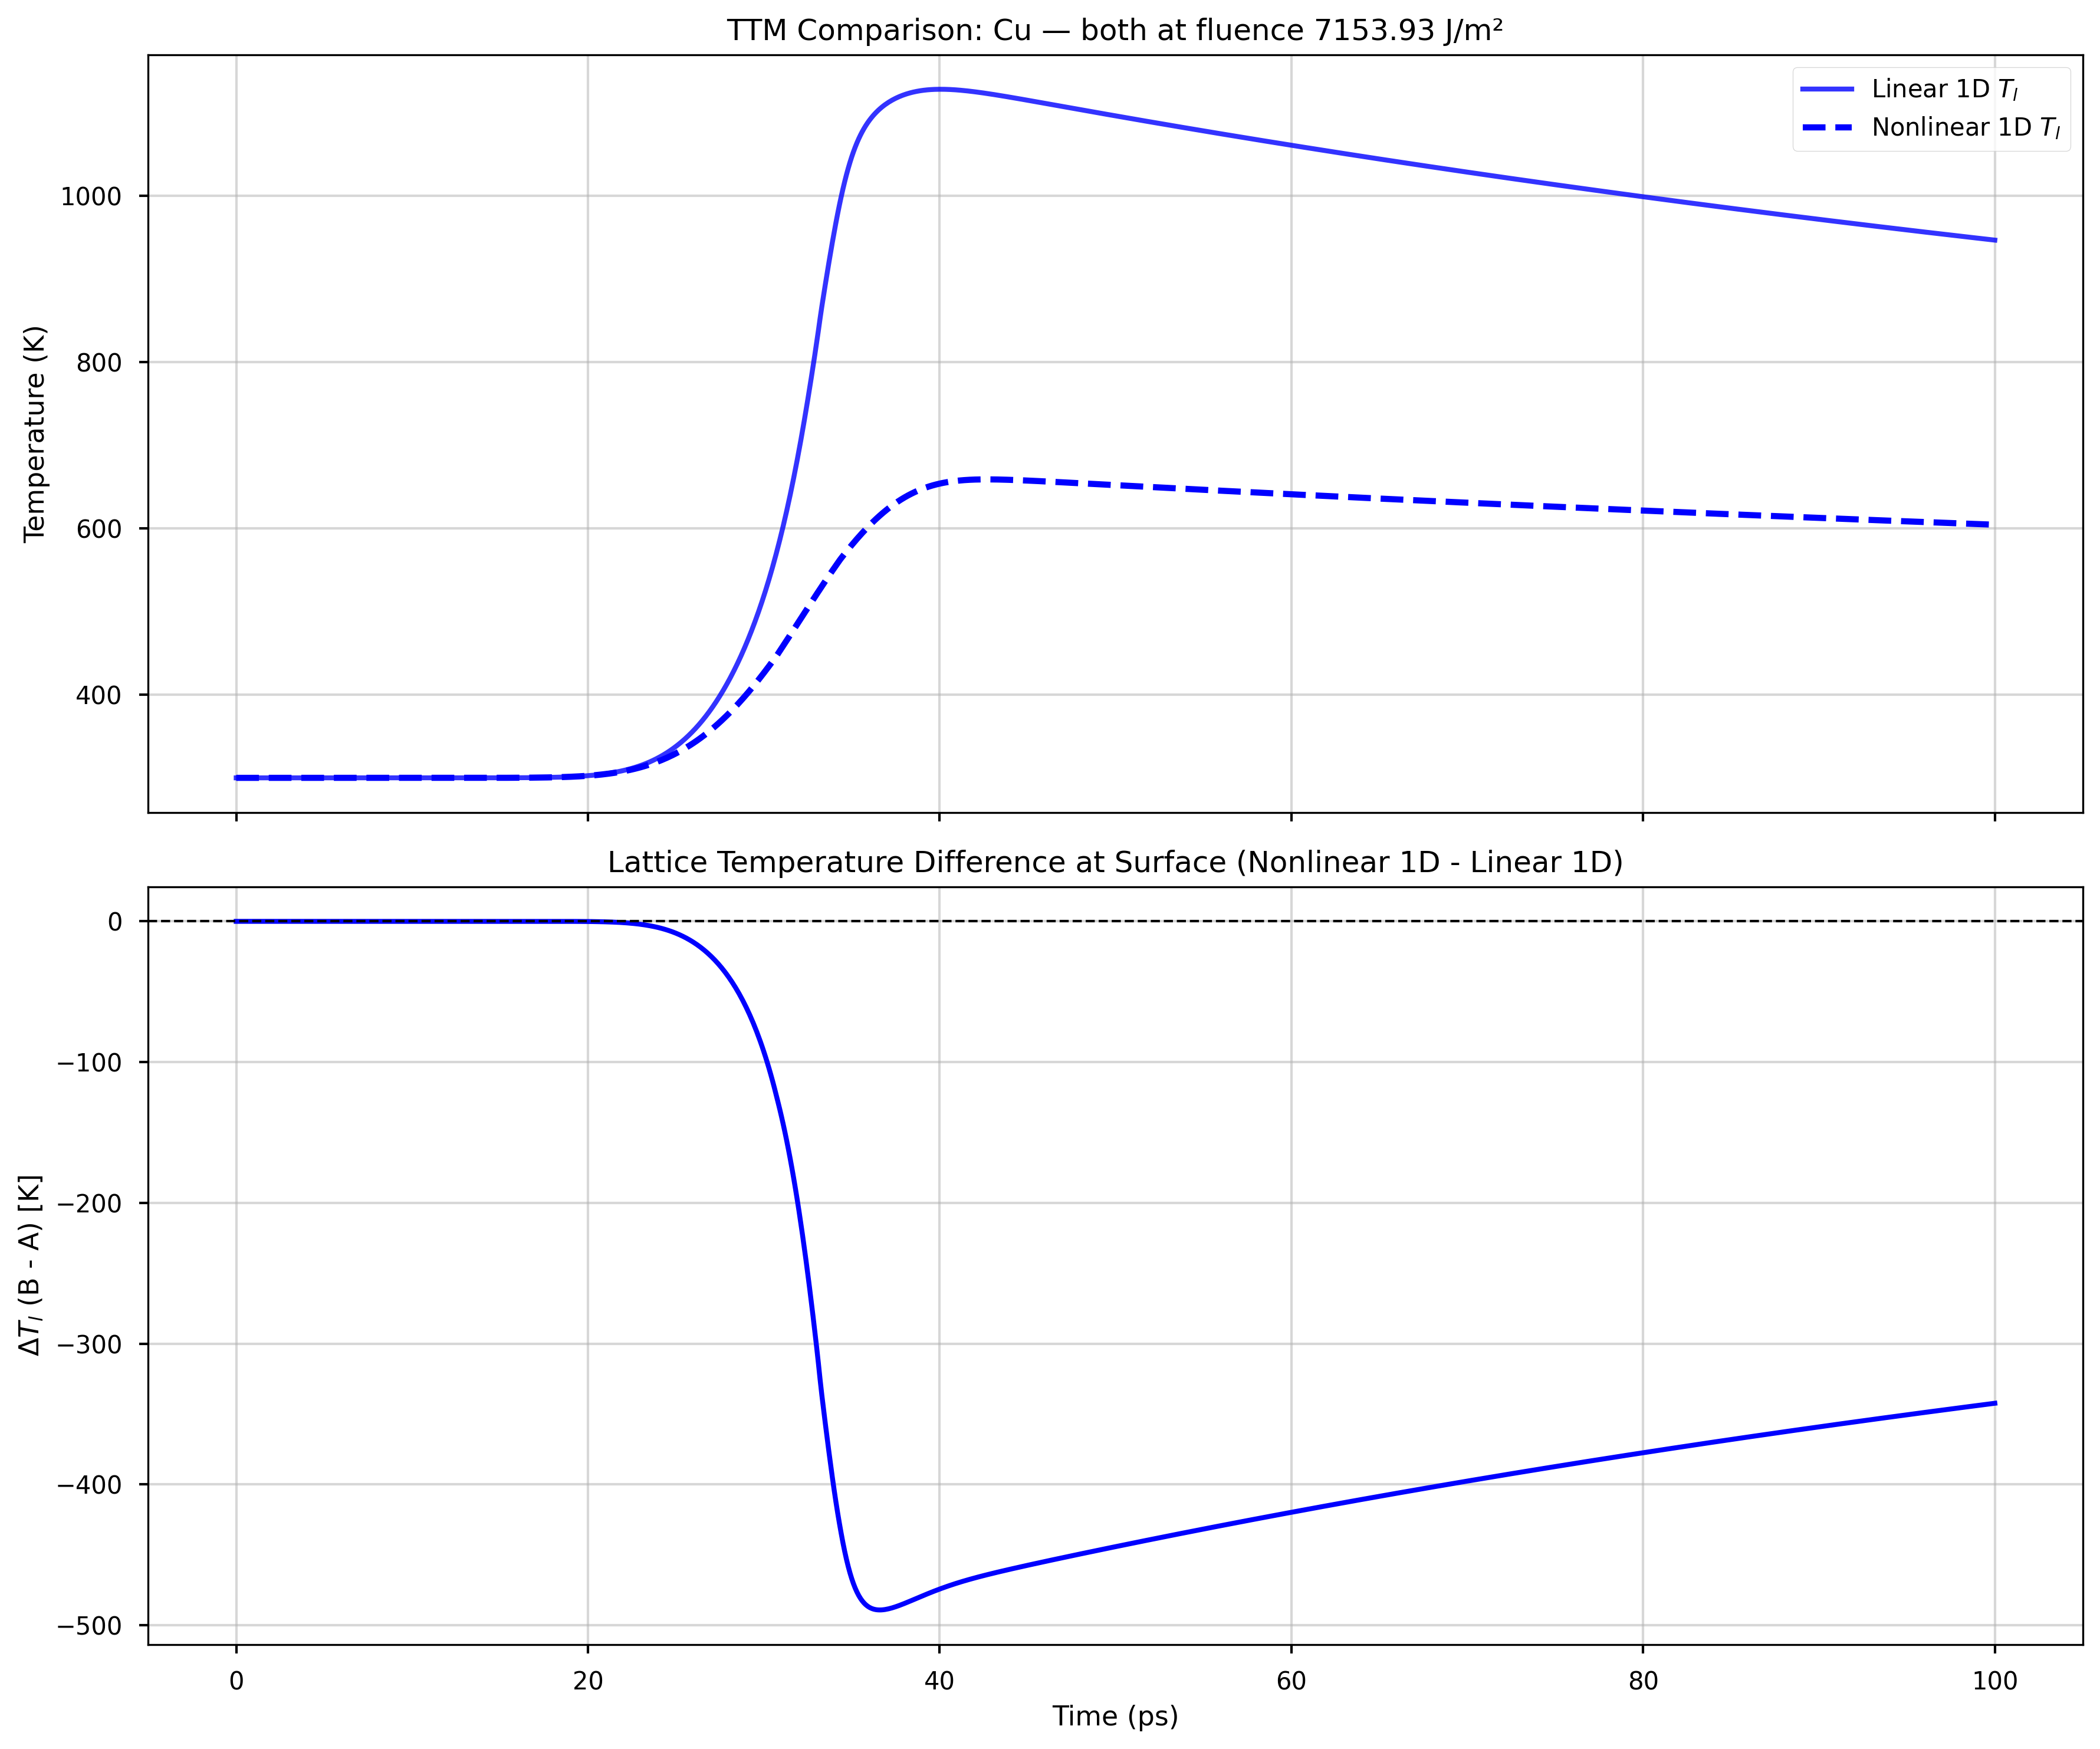
\includegraphics[width=0.32\linewidth]{figures/ch3/comparison_Cu_linear_vs_nonlinear_1d.png}
    }
    \caption{Comparison of 1D linear and 1D nonlinear pTTM predictions at the common fluence \(\hat F_{\mathrm{th}}^{\mathrm{1D,lin}}\) for each material. The upper panels show the surface lattice-temperature histories, and the lower panels show \(\Delta T_l(t)=T_l^{\mathrm{nl}}-T_l^{\mathrm{lin}}\).}
    \label{fig:ch3-comparison-linear-vs-nonlinear-1d-metals}
\end{figure}

\begin{figure}[H]
    \centering
    \subfloat[Au.\label{fig:ch3-comparison-linear-vs-nonlinear-2d-au}]{%
        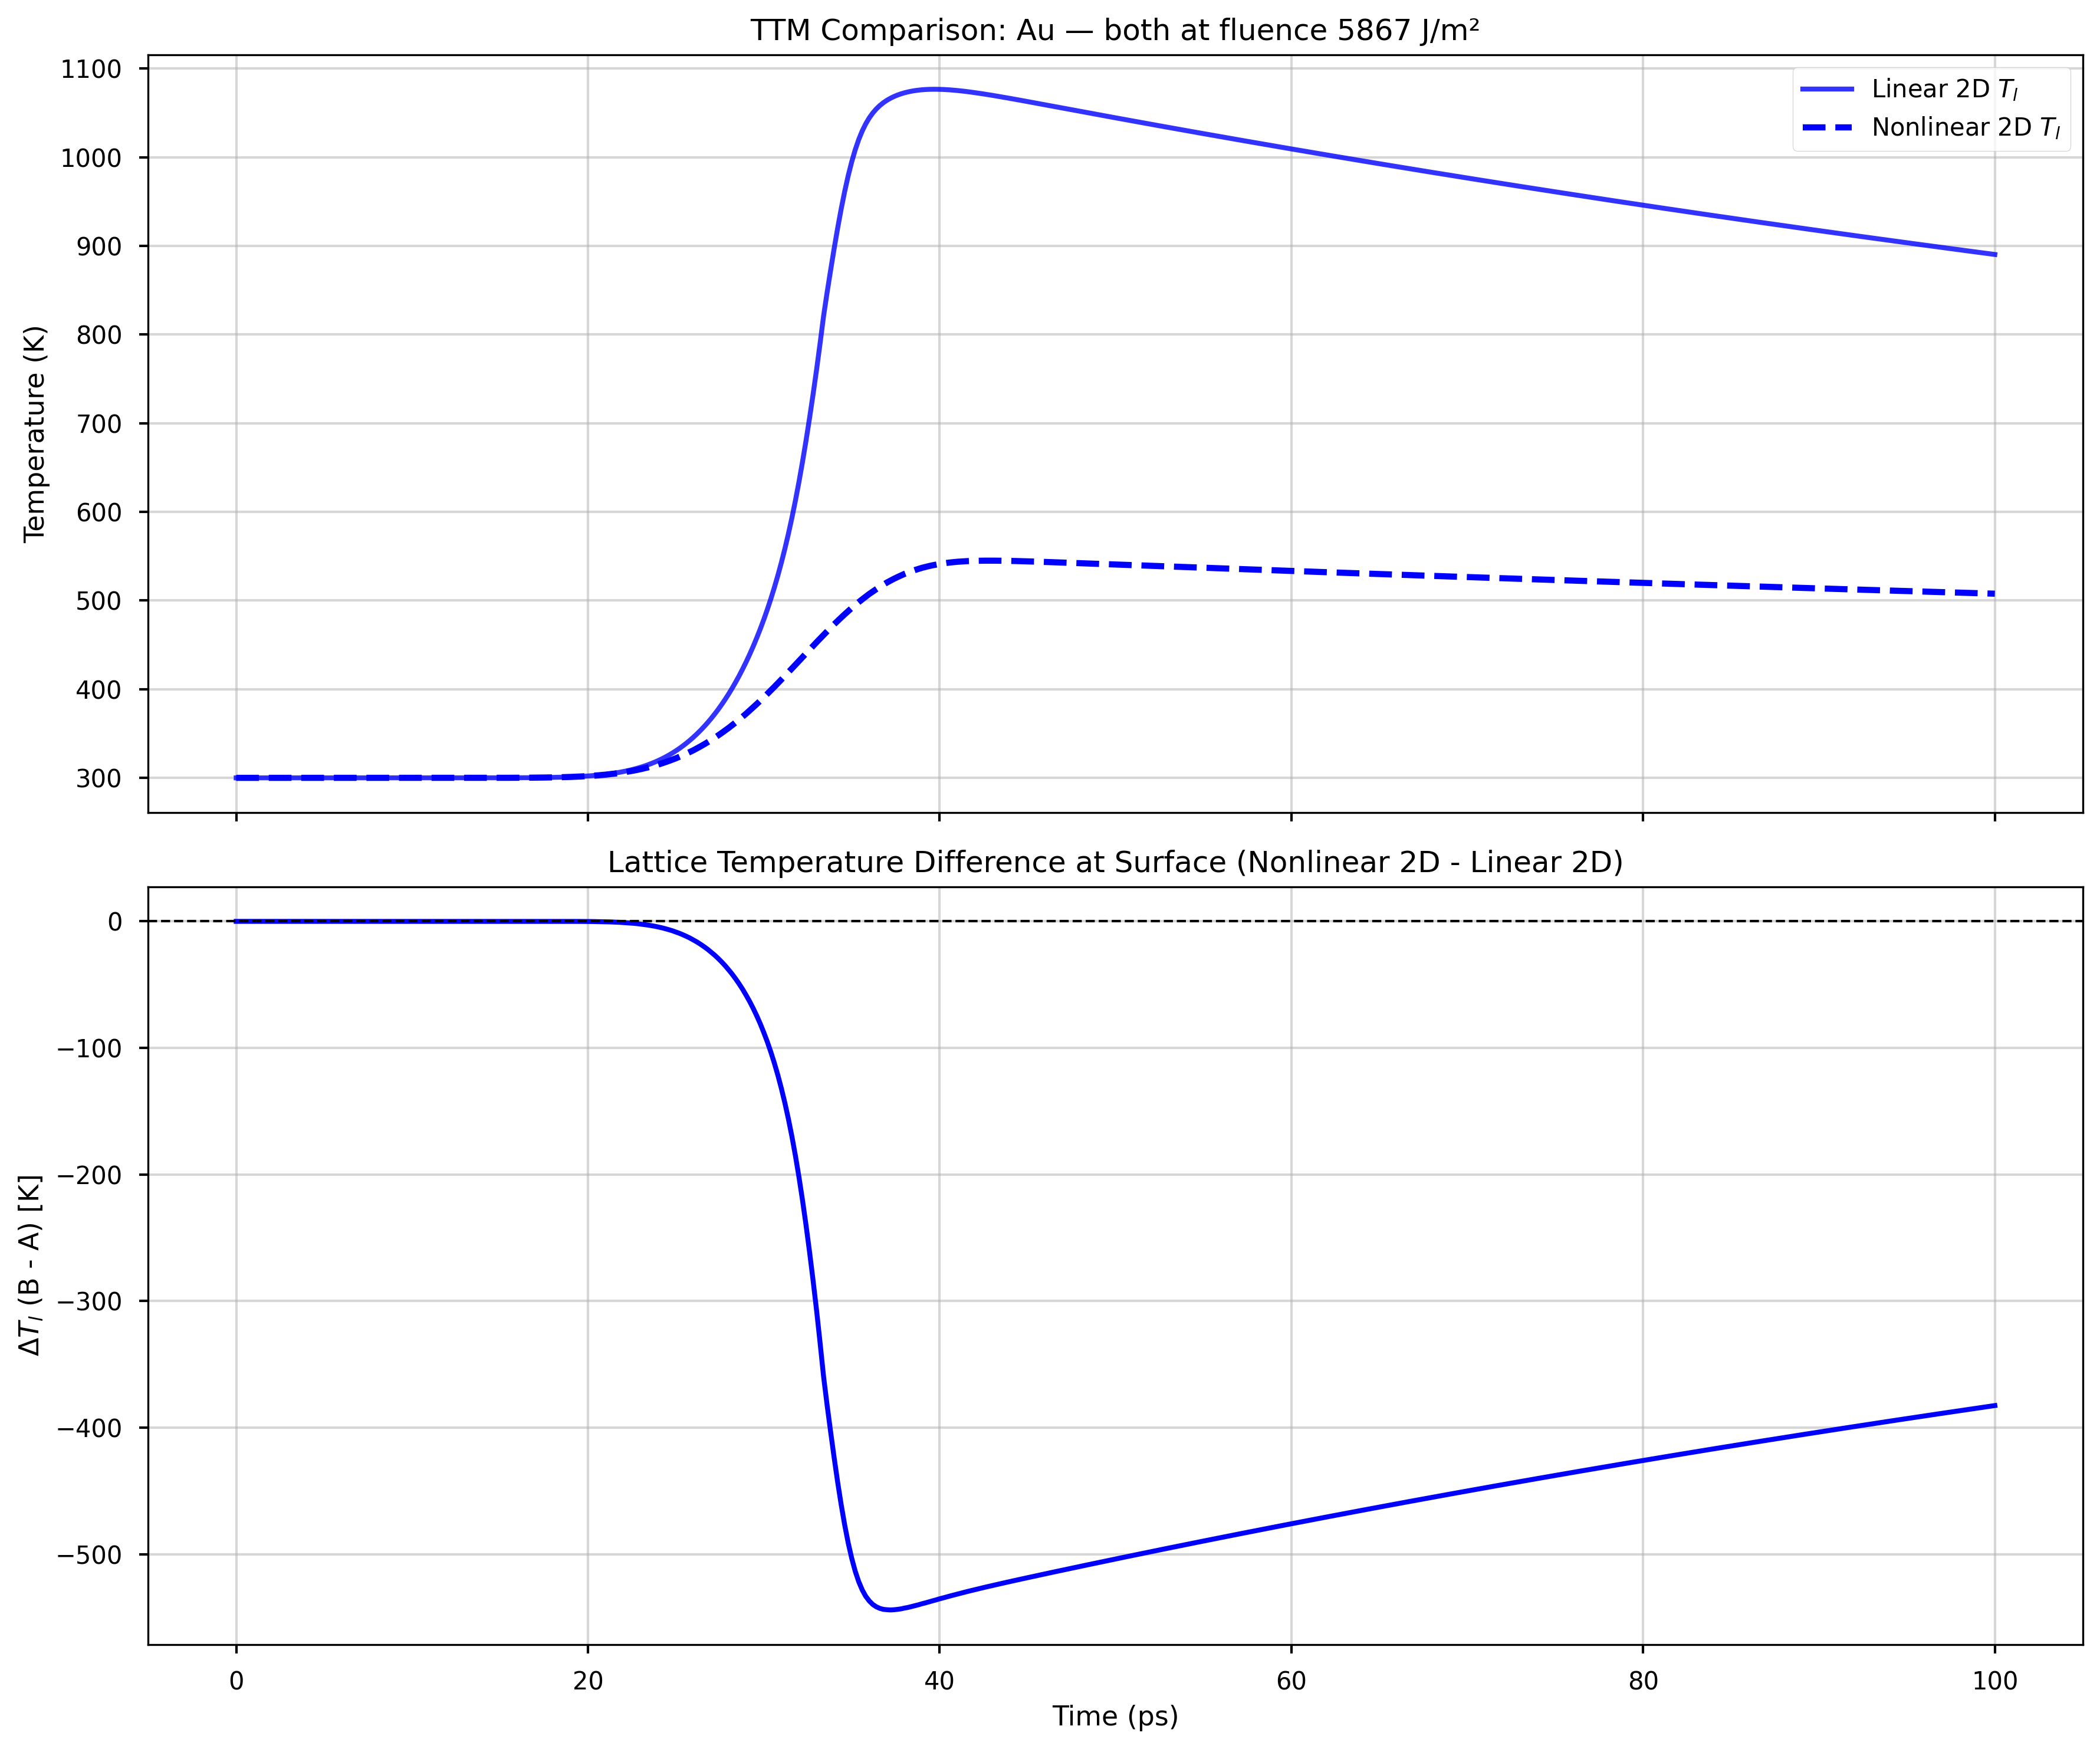
\includegraphics[width=0.32\linewidth]{figures/ch3/comparison_Au_linear_vs_nonlinear_2d.png}
    }\hfill
    \subfloat[Ni.\label{fig:ch3-comparison-linear-vs-nonlinear-2d-ni}]{%
        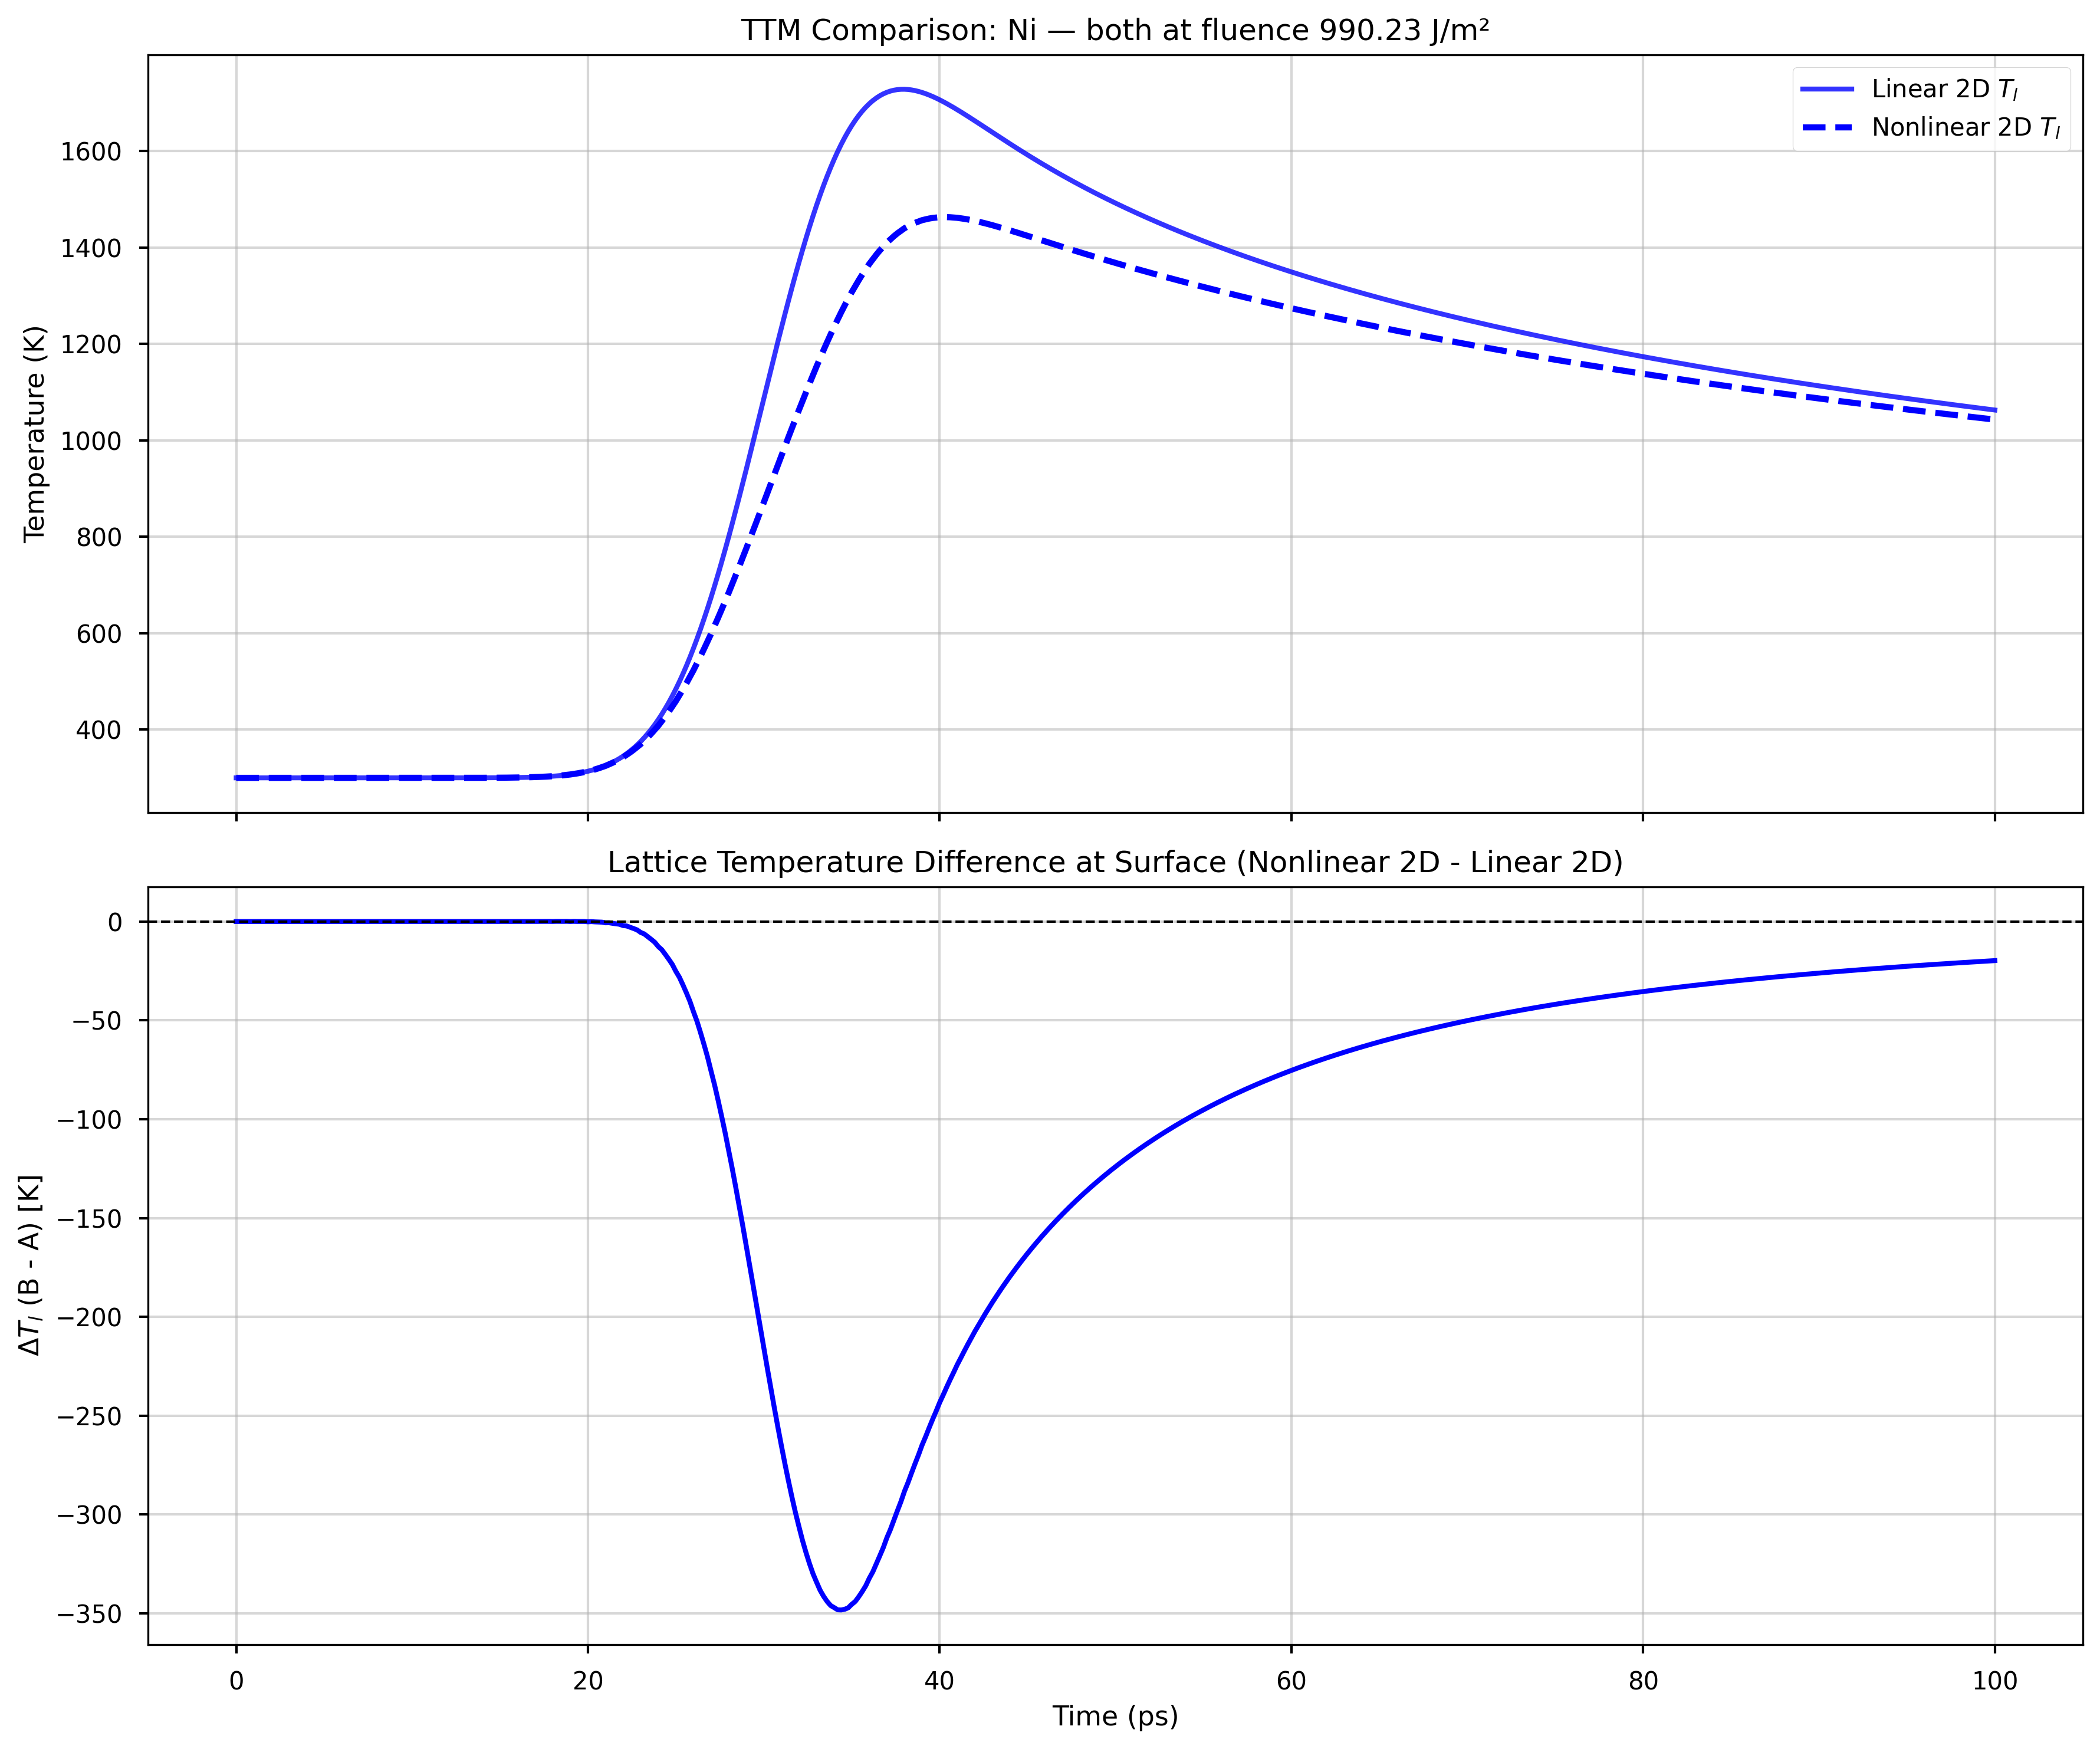
\includegraphics[width=0.32\linewidth]{figures/ch3/comparison_Ni_linear_vs_nonlinear_2d.png}
    }\hfill
    \subfloat[Cu.\label{fig:ch3-comparison-linear-vs-nonlinear-2d-cu}]{%
        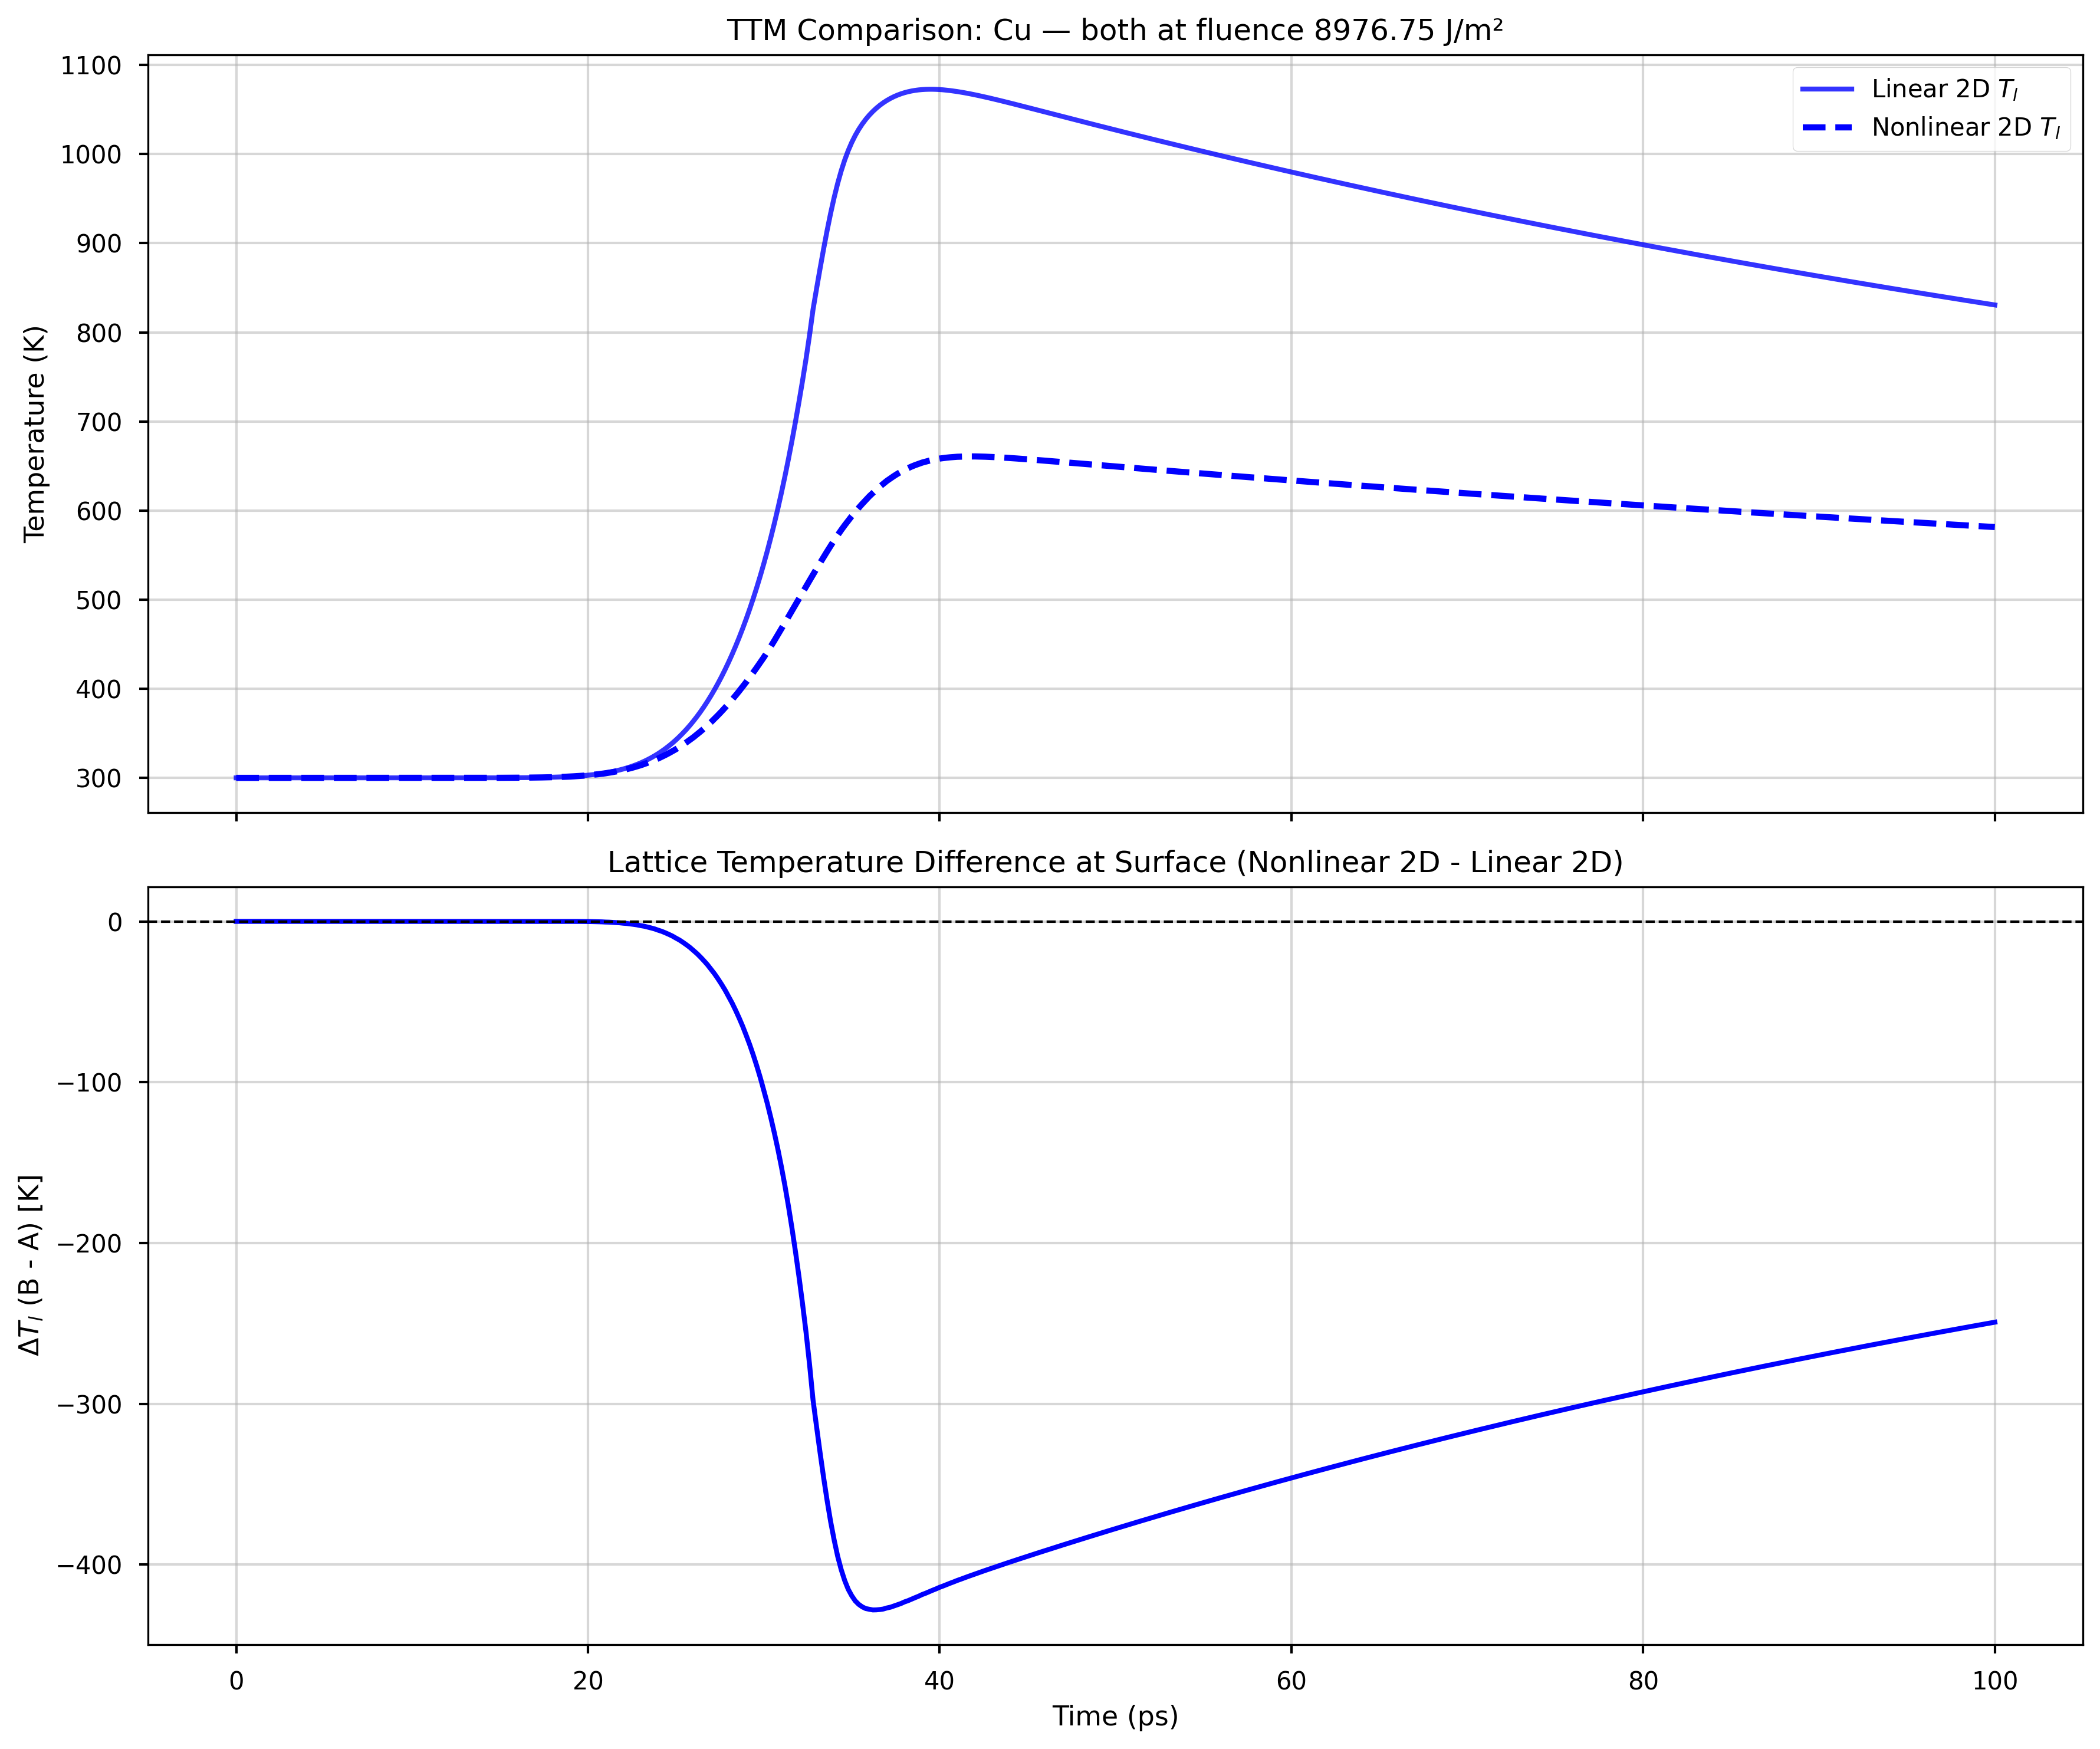
\includegraphics[width=0.32\linewidth]{figures/ch3/comparison_Cu_linear_vs_nonlinear_2d.png}
    }
    \caption{Comparison of 2D linear and 2D nonlinear pTTM predictions at the common fluence \(\hat F_{\mathrm{th}}^{\mathrm{2D,lin}}\) for each material. The upper panels show the representative surface lattice-temperature histories, and the lower panels show \(\Delta T_l(t)=T_l^{\mathrm{nl}}-T_l^{\mathrm{lin}}\).}
    \label{fig:ch3-comparison-linear-vs-nonlinear-2d-metals}
\end{figure}

\subsubsection{Implications for threshold estimation}
\label{sec:ch3-ablation-discussion-implications}

The linear model systematically underpredicts the incident
fluence required to reach the melting criterion, and the discrepancy is
particularly strong for Au and Cu. A more defensible interpretation is
that the linear model provides a computationally inexpensive lower-bound
predictor and an effective initialisation for the threshold search, while
the nonlinear model is required whenever one seeks quantitatively credible
threshold values.

At the same time, the results show that dimensionality and constitutive
nonlinearity affect the threshold in different ways. The 1D/2D correction
is large for Au and Cu but small for Ni, whereas the linear/nonlinear
correction is substantial for all three materials. For the present
configuration, model-form sensitivity is therefore more systematic than
dimensional sensitivity.

Finally, comparison with experiment should be interpreted with care.
The values reported here are melting-onset thresholds defined by
\(T_{l,\max}\ge T_m\), rather than direct material-removal thresholds.
Moreover, the simulations use a \(\SI{10}{\pico\second}\) pulse, whereas
much of the ablation-threshold literature concerns femtosecond excitation
\cite{Hashida_2001,Gamaly_2002,Forster_2021}. Reported experimental
thresholds may also differ according to whether incident or absorbed
fluence is quoted. The present results should therefore be understood as
model-based thermal threshold indicators for the chosen pulse regime,
rather than as direct one-to-one predictions of experimental ablation
thresholds.
